\documentclass[portrait,final,archD,fontscale=0.477]{baposter}
% Currently set to 24" wide by 36" tall (archD).
% See baposter.cls for info on changing paper dimensions

\usepackage{amsmath}
\usepackage{subcaption}
\usepackage[utf8]{inputenc}
\usepackage{pgfplots}
\usepgfplotslibrary{patchplots,colormaps}
\DeclareUnicodeCharacter{2212}{−}
\usepgfplotslibrary{groupplots,dateplot}
\usetikzlibrary{patterns,shapes.arrows}
\pgfplotsset{compat=newest}
\usepackage{adjustbox}
\usepackage{csquotes}
\renewcommand{\mkbegdispquote}[2]{\itshape}
\usepackage{natbib}
%\usepackage[style=authoryear-icomp,maxbibnames=9,maxcitenames=2,backend=biber]{biblatex}



\usepackage{calc}
\usepackage{graphicx}
\usepackage{amsmath}
\usepackage{amssymb}
\usepackage{relsize}
\usepackage{multirow}
\usepackage{rotating}
\usepackage{bm}
\usepackage{url}
\usepackage{subcaption}

\usepackage{graphicx}
\usepackage{multicol}

%\usepackage{times}
%\usepackage{helvet}
%\usepackage{bookman}
\usepackage{palatino}
\newmintedfile{cpp}{
  fontsize=\scriptsize,
}

\usepackage{etoolbox}
\patchcmd{\thebibliography}{\section*{\refname}}{}{}{}
%\newcommand{\captionfont}{\footnotesize}

%%%%%%%%%%%%%%%%%%%%%%%%%%%%%%%%%%%%%%%%%%%%%%%%%%%%%%%%%%%%%%%%%%%%%%%%%%%%%%%%
%%%% Some math symbols used in the text
%%%%%%%%%%%%%%%%%%%%%%%%%%%%%%%%%%%%%%%%%%%%%%%%%%%%%%%%%%%%%%%%%%%%%%%%%%%%%%%%

%%%%%%%%%%%%%%%%%%%%%%%%%%%%%%%%%%%%%%%%%%%%%%%%%%%%%%%%%%%%%%%%%%%%%%%%%%%%%%%%
% Multicol Settings
%%%%%%%%%%%%%%%%%%%%%%%%%%%%%%%%%%%%%%%%%%%%%%%%%%%%%%%%%%%%%%%%%%%%%%%%%%%%%%%%
\setlength{\columnsep}{1.5em}
\setlength{\columnseprule}{0mm}

%%%%%%%%%%%%%%%%%%%%%%%%%%%%%%%%%%%%%%%%%%%%%%%%%%%%%%%%%%%%%%%%%%%%%%%%%%%%%%%%
% Save space in lists. Use this after the opening of the list
%%%%%%%%%%%%%%%%%%%%%%%%%%%%%%%%%%%%%%%%%%%%%%%%%%%%%%%%%%%%%%%%%%%%%%%%%%%%%%%%
\newcommand{\compresslist}{%
\setlength{\itemsep}{1pt}%
\setlength{\parskip}{0pt}%
\setlength{\parsep}{0pt}%
}

%%%%%%%%%%%%%%%%%%%%%%%%%%%%%%%%%%%%%%%%%%%%%%%%%%%%%%%%%%%%%%%%%%%%%%%%%%%%%%
%%% Begin of Document
%%%%%%%%%%%%%%%%%%%%%%%%%%%%%%%%%%%%%%%%%%%%%%%%%%%%%%%%%%%%%%%%%%%%%%%%%%%%%%

\begin{document}

%%%%%%%%%%%%%%%%%%%%%%%%%%%%%%%%%%%%%%%%%%%%%%%%%%%%%%%%%%%%%%%%%%%%%%%%%%%%%%
%%% Here starts the poster
%%%---------------------------------------------------------------------------
%%% Format it to your taste with the options
%%%%%%%%%%%%%%%%%%%%%%%%%%%%%%%%%%%%%%%%%%%%%%%%%%%%%%%%%%%%%%%%%%%%%%%%%%%%%%
% Define some colors

\definecolor{stevensred}{rgb}{0.639, 0.149, 0.219}
\definecolor{stevensgray}{rgb}{0.60392, 0.596, 0.60392}
\definecolor{burgundy}{rgb}{0.5, 0.0, 0.13}
\definecolor{brightmaroon}{rgb}{0.76, 0.13, 0.28}
\definecolor{mediumcandyapplered}{rgb}{0.89, 0.02, 0.17}

%%
\begin{poster}%
  % Poster Options
  {
    % Show grid to help with alignment
    grid=false,
    % Column spacing
    colspacing=1em,
    % Color style
    bgColorOne=white,
    bgColorTwo=white,
    borderColor=stevensgray,
    headerColorOne=mediumcandyapplered,
    headerColorTwo=mediumcandyapplered,
    headerFontColor=white,
    boxColorOne=white,
    boxColorTwo=stevensgray,
    % Format of textbox
    textborder=rectangle,
    % Format of text header
    eyecatcher=true,
    headerborder=closed,
    headerheight=0.1\textheight,
    %  textfont=\sc, An example of changing the text font
    headershape=rectangle,
    headershade=plain,
    headerfont=\Large\bf\textsc, %Sans Serif
    textfont={\setlength{\parindent}{1.5em}},
    boxshade=plain,
    %  background=shade-tb,
    background=plain,
    linewidth=2pt
  }
  % Eye Catcher
  {\begin{minipage}{8em}
      \hfill\vspace{1in}
    \end{minipage} } % Empty space, replace with image if desired
  % Title
  {\bf \textsc{  Comparing the costs of abstraction for DL frameworks } }
  % Authors
  {\textsc{  Maksim Levental and Elena Orlova \\ University of Chicago, Chicago IL}}
  % University logo
  {% The makebox allows the title to flow into the logo, this is a hack because of the L shaped logo.
    
\includegraphics[height=9.0em]{figures/uchicago_seal.jpg}
  }

  %%%%%%%%%%%%%%%%%%%%%%%%%%%%%%%%%%%%%%%%%%%%%%%%%%%%%%%%%%%%%%%%%%%%%%%%%%%%%%
  %%% Now define the boxes that make up the poster
  %%%---------------------------------------------------------------------------
  %%% Each box has a name and can be placed absolutely or relatively.
  %%% The only inconvenience is that you can only specify a relative position
  %%% towards an already declared box. So if you have a box attached to the
  %%% bottom, one to the top and a third one which should be in between, you
  %%% have to specify the top and bottom boxes before you specify the middle
  %%% box.
  %%%%%%%%%%%%%%%%%%%%%%%%%%%%%%%%%%%%%%%%%%%%%%%%%%%%%%%%%%%%%%%%%%%%%%%%%%%%%%
  %
  % A coloured circle useful as a bullet with an adjustably strong filling
  \newcommand{\colouredcircle}{%
    \tikz{\useasboundingbox (-0.2em,-0.32em) rectangle(0.2em,0.32em); \draw[draw=black,fill=lightblue,line width=0.03em] (0,0) circle(0.18em);}}

  %%%%%%%%%%%%%%%%%%%%%%%%%%%%%%%%%%%%%%%%%%%%%%%%%%%%%%%%%%%%%%%%%%%%%%%%%%%%%%
  \headerbox{Introduction}{name=problem,column=0,row=0}{
    %%%%%%%%%%%%%%%%%%%%%%%%%%%%%%%%%%%%%%%%%%%%%%%%%%%%%%%%%%%%%%%%%%%%%%%%%%%%%%

    Deep Learning (DL) frameworks represent neural network models as dataflow and computation graphs (where nodes correspond to functional units and edges correspond to composition).
    In recent years, there has been a proliferation of DL frameworks implemented as domain-specific languages (DSLs) embedded in ``high-level'' languages such as Python, Java, and C\#.
    These DSLs serve as abstractions that aim to map the DL graphs to hardware pipelines.
    That is to say, they hide details of DL models that are judged to be either irrelevant or too onerous to consider.
    Thus, our intent here is to investigate the costs of some of the abstractions employed by framework developers.
    In particular we focus on the PyTorch framework and ecosystem deployed to GPUs.

  }

  %%%%%%%%%%%%%%%%%%%%%%%%%%%%%%%%%%%%%%%%%%%%%%%%%%%%%%%%%%%%%%%%%%%%%%%%%%%%%%
  \headerbox{References}{name=references,column=0,above=bottom}{
    %%%%%%%%%%%%%%%%%%%%%%%%%%%%%%%%%%%%%%%%%%%%%%%%%%%%%%%%%%%%%%%%%%%%%%%%%%%%%%
    \smaller
    \bibliographystyle{science}
    \bibliography{main}
  }

  %%%%%%%%%%%%%%%%%%%%%%%%%%%%%%%%%%%%%%%%%%%%%%%%%%%%%%%%%%%%%%%%%%%%%%%%%%%%%%
  \headerbox{CUDA semantics and ResNet-50}{name=method,column=0,below=problem, above=references}{
    %%%%%%%%%%%%%%%%%%%%%%%%%%%%%%%%%%%%%%%%%%%%%%%%%%%%%%%%%%%%%%%%%%%%%%%%%%%%%%

    \begin{figure}[H]
      \centering
      \cppfile{code/softmax.c}
      \caption{Softmax loss CUDA kernel}
      \label{fig:cuda_hello_world}
    \end{figure}
    \begin{figure}[H]
      \centering
      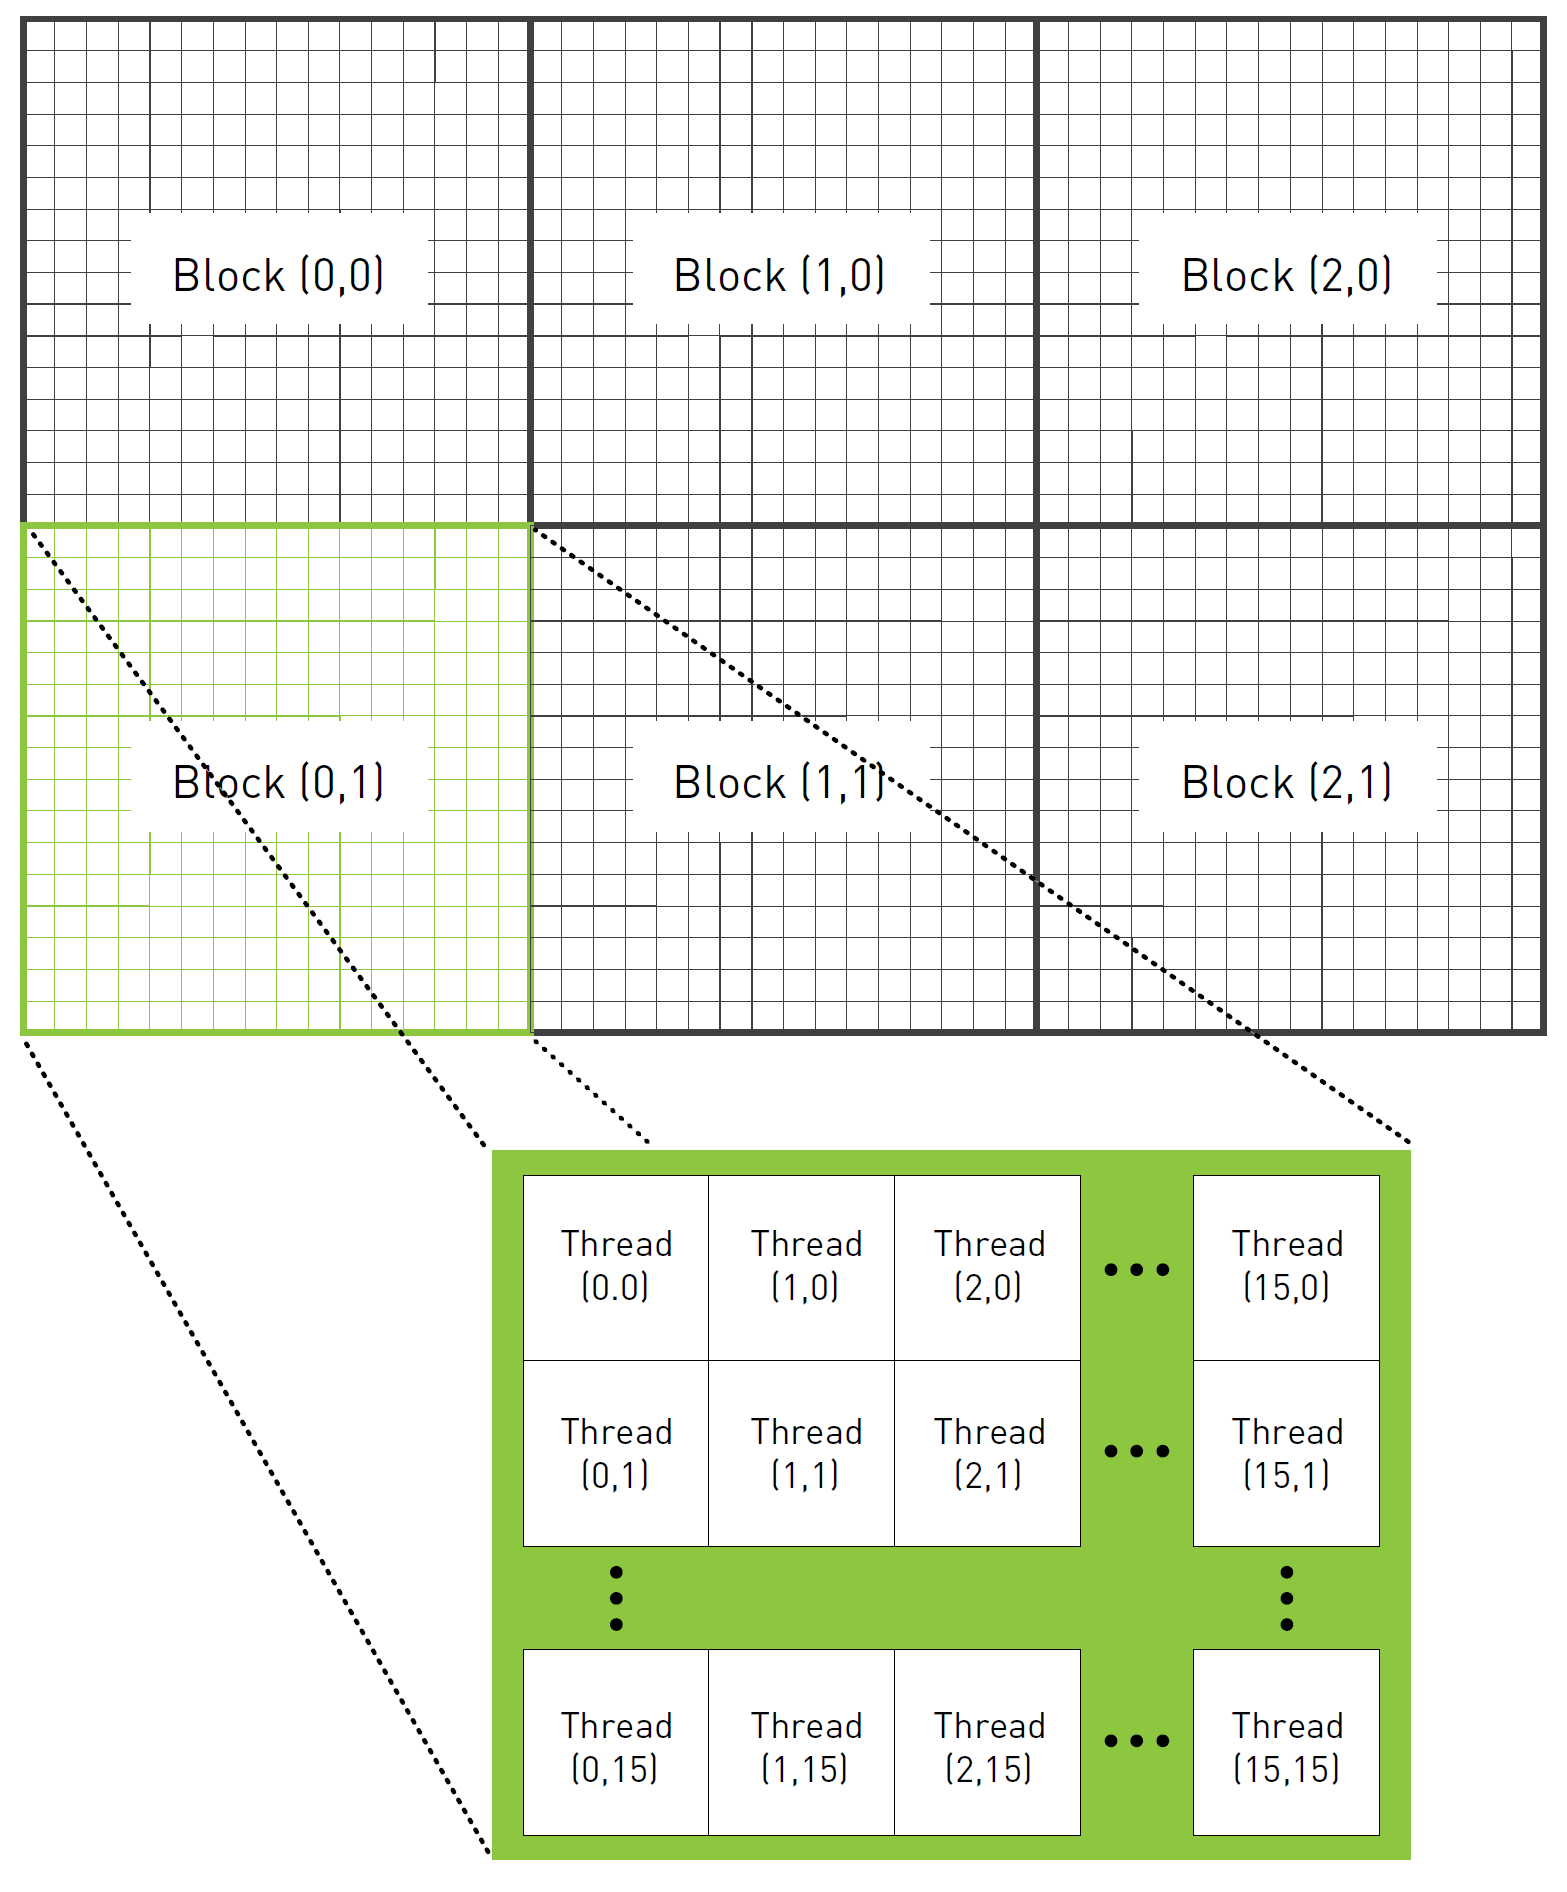
\includegraphics[width=.7\linewidth]{figures/matrix_thread.png}
      \caption{Mapping from thread and block to matrix element~\cite{10.5555/1891996}.}\label{fig:figure}
    \end{figure}
    \begin{figure}[H]
      \centering
      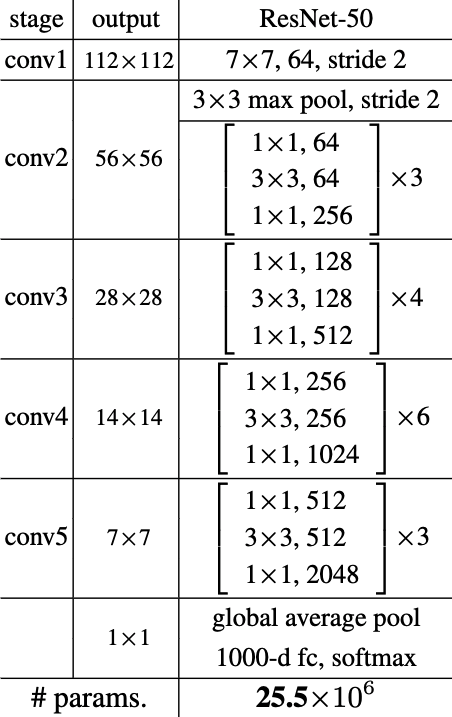
\includegraphics[width=0.5\linewidth]{figures/resnet50.png}
      \caption{ResNet-50 network architecture~\cite{he2015deep}. Note that each convolution is followed by a batch normalization unit and each ``stage'' is followed by a ReLU (residual connections omitted).}\label{fig:resnet}
    \end{figure}

  }

  %%%%%%%%%%%%%%%%%%%%%%%%%%%%%%%%%%%%%%%%%%%%%%%%%%%%%%%%%%%%%%%%%%%%%%%%%%%%%%
  \headerbox{Methods}{name=results,column=1,span=2,row=0}{
    %%%%%%%%%%%%%%%%%%%%%%%%%%%%%%%%%%%%%%%%%%%%%%%%%%%%%%%%%%%%%%%%%%%%%%%%%%%%%%

    \begin{multicols}{2}
      We implement the popular object detection deep neural network ResNet-50~\cite{he2015deep} at four levels of abstraction (PyTorch, TorchScript\footnote{TorchScript models are serializations of PyTorch models but can run in inference mode in C++, i.e. sans Python runtime.}, LibTorch, and cuDNN) in order to investigate the differences amongst them.
      We measure accuracy, execution time, GPU utilization, and memory efficiency of each implementation on four image datasets (MNIST, CIFAR10, STL10, PASCAL).
      The source for the implementations is available on GitHub\footnote{\url{https://github.com/makslevental/pytorch_abstraction_comparison}}.
      The datasets were chosen because they span the spectrum of image complexity (from small single-channel images to large multi-channel images).
      The reasons for choosing ResNet-50 are two fold.
      Firstly, it serves as a benchmark architecture in the research community.
      Secondly, it includes functional units included in many other network architectures (residual units, convolutions of various sizes, batch normalizations, ReLU activations, and pooling layers) and is therefore representative of typical neural network compute workloads.
    \end{multicols}

  }

  %%%%%%%%%%%%%%%%%%%%%%%%%%%%%%%%%%%%%%%%%%%%%%%%%%%%%%%%%%%%%%%%%%%%%%%%%%%%%%
  \headerbox{Experimental Results}{name=background model,column=1, span=2,below=results, above=bottom}{
    %%%%%%%%%%%%%%%%%%%%%%%%%%%%%%%%%%%%%%%%%%%%%%%%%%%%%%%%%%%%%%%%%%%%%%%%%%%%%%
    The PyTorch implementation compares \textbf{favorably} with both LibTorch and the cuDNN implementations in terms of accuracy.
    On MNIST and CIFAR10 all three implementations perform reasonably well;
    LibTorch and PyTorch attain maximum accuracy at around the same time while cuDNN lags behind.
    In terms of execution time and memory usage PyTorch compares \textbf{unfavorably} with each of the other implementations.
    We measure execution time, memory usage, and GPU utilization during evaluation on PASCAL for various batch sizes and resolution.
    \begin{figure}[H]
      \centering
      \begin{subfigure}{0.24\linewidth}
        \centering
        \begin{adjustbox}{width=\textwidth}
          % This file was created by tikzplotlib v0.9.5.
\begin{tikzpicture}





\begin{axis}[
axis background/.style={fill=white!89.8039215686275!black},
axis line style={white},
legend cell align={left},
legend style={fill opacity=0.8, draw opacity=1, text opacity=1, at={(0.03,0.03)}, anchor=south west, draw=white!80!black, fill=white!89.8039215686275!black},
%log basis y={10},
tick align=outside,
tick pos=left,
title={MNIST training},
x grid style={white},
xlabel={time},
xmajorgrids,
xmin=-1.8444581, xmax=48.6648733,
xtick style={color=white!33.3333333333333!black},
y grid style={white},
ylabel={accuracy},
ymajorgrids,
ymin=23.6870160941979, ymax=107.098952012845,
%ymode=log,
ytick style={color=white!33.3333333333333!black}
]
\path [fill=cudnn, fill opacity=0.2, very thin]
(axis cs:0.4782266,70.409309)
--(axis cs:0.4782266,25.368546)
--(axis cs:0.9232159,52.610394)
--(axis cs:1.3681511,46.064877)
--(axis cs:1.813181,59.719769)
--(axis cs:2.2582623,72.457542)
--(axis cs:2.7032656,79.869225)
--(axis cs:3.1482741,86.851219)
--(axis cs:3.5932938,91.06488)
--(axis cs:4.038329,84.553329)
--(axis cs:4.4834467,93.05027)
--(axis cs:4.9285291,95.606316)
--(axis cs:5.3737088,95.278534)
--(axis cs:5.8189509,96.363792)
--(axis cs:6.2641013,96.418137)
--(axis cs:6.7093389,96.908966)
--(axis cs:7.1544196,77.438858)
--(axis cs:7.5995075,92.370926)
--(axis cs:8.0445662,94.998299)
--(axis cs:8.489797,96.7714)
--(axis cs:8.9349618,97.246941)
--(axis cs:9.3799734,97.257133)
--(axis cs:9.8251089,97.623978)
--(axis cs:10.2701673,97.712296)
--(axis cs:10.7152981,97.73098)
--(axis cs:11.1603761,97.7089)
--(axis cs:11.6055043,97.715691)
--(axis cs:12.0506865,97.829483)
--(axis cs:12.4958184,97.832878)
--(axis cs:12.9409165,96.295853)
--(axis cs:13.3859977,97.927986)
--(axis cs:13.8311519,97.729279)
--(axis cs:14.2761924,98.254074)
--(axis cs:14.7213617,97.005775)
--(axis cs:15.1664679,98.388245)
--(axis cs:15.6114732,98.25238)
--(axis cs:16.0566084,98.410324)
--(axis cs:16.501812,98.552986)
--(axis cs:16.9470843,98.328804)
--(axis cs:17.3922826,98.226906)
--(axis cs:17.8373712,97.515282)
--(axis cs:18.282443,98.357674)
--(axis cs:18.7275257,98.49015)
--(axis cs:19.1725744,98.372963)
--(axis cs:19.6176348,98.576767)
--(axis cs:20.0626668,98.637909)
--(axis cs:20.5078902,98.340691)
--(axis cs:20.9531108,98.422218)
--(axis cs:21.398351,98.510529)
--(axis cs:21.843595,98.739807)
--(axis cs:22.2887302,98.524117)
--(axis cs:22.7337989,98.707542)
--(axis cs:23.1789517,98.603943)
--(axis cs:23.6240882,98.758492)
--(axis cs:24.0692921,98.683762)
--(axis cs:24.5144183,98.773781)
--(axis cs:24.9595631,96.908966)
--(axis cs:25.4046424,98.656593)
--(axis cs:25.8497148,97.922897)
--(axis cs:26.2947474,98.629417)
--(axis cs:26.7398837,98.894363)
--(axis cs:27.1848716,98.77887)
--(axis cs:27.6299501,98.751701)
--(axis cs:28.0749458,98.945312)
--(axis cs:28.5199763,97.365829)
--(axis cs:28.9651299,96.110733)
--(axis cs:29.4101996,98.704147)
--(axis cs:29.8552906,98.901154)
--(axis cs:30.3002666,98.972488)
--(axis cs:30.7453382,99.031929)
--(axis cs:31.190327,97.476219)
--(axis cs:31.6354719,99.040421)
--(axis cs:32.0805844,98.158966)
--(axis cs:32.5257041,98.904549)
--(axis cs:32.9708542,99.011551)
--(axis cs:33.4160196,99.09137)
--(axis cs:33.8610718,99.217049)
--(axis cs:34.3061513,99.118546)
--(axis cs:34.7512437,89.349525)
--(axis cs:35.1961926,95.864471)
--(axis cs:35.6411077,98.028191)
--(axis cs:36.0860932,98.462975)
--(axis cs:36.5310712,98.615829)
--(axis cs:36.9761031,98.085938)
--(axis cs:37.4211117,98.965691)
--(axis cs:37.8660675,98.994568)
--(axis cs:38.3110037,99.011551)
--(axis cs:38.7560695,99.188179)
--(axis cs:39.2011195,99.077782)
--(axis cs:39.6460269,99.099861)
--(axis cs:40.0909067,99.284988)
--(axis cs:40.5359762,98.972488)
--(axis cs:40.9810362,99.191574)
--(axis cs:41.4260278,99.235733)
--(axis cs:41.8710576,99.135529)
--(axis cs:42.316014,99.179688)
--(axis cs:42.760984,94.772415)
--(axis cs:43.2059163,98.907951)
--(axis cs:43.6508853,99.094772)
--(axis cs:44.0959597,98.220108)
--(axis cs:44.5409831,99.150818)
--(axis cs:44.5409831,99.867531)
--(axis cs:44.5409831,99.867531)
--(axis cs:44.0959597,99.835258)
--(axis cs:43.6508853,99.852242)
--(axis cs:43.2059163,99.821671)
--(axis cs:42.760984,99.874321)
--(axis cs:42.316014,99.853943)
--(axis cs:41.8710576,99.83696)
--(axis cs:41.4260278,99.808083)
--(axis cs:40.9810362,99.806389)
--(axis cs:40.5359762,99.84375)
--(axis cs:40.0909067,99.819969)
--(axis cs:39.6460269,99.802986)
--(axis cs:39.2011195,99.816574)
--(axis cs:38.7560695,99.842049)
--(axis cs:38.3110037,99.804688)
--(axis cs:37.8660675,99.796196)
--(axis cs:37.4211117,99.813179)
--(axis cs:36.9761031,99.772415)
--(axis cs:36.5310712,99.758835)
--(axis cs:36.0860932,99.772415)
--(axis cs:35.6411077,99.845451)
--(axis cs:35.1961926,99.797897)
--(axis cs:34.7512437,99.729958)
--(axis cs:34.3061513,99.774117)
--(axis cs:33.8610718,99.808083)
--(axis cs:33.4160196,99.733353)
--(axis cs:32.9708542,99.750343)
--(axis cs:32.5257041,99.733353)
--(axis cs:32.0805844,99.721466)
--(axis cs:31.6354719,99.729958)
--(axis cs:31.190327,99.801292)
--(axis cs:30.7453382,99.772415)
--(axis cs:30.3002666,99.735054)
--(axis cs:29.8552906,99.711281)
--(axis cs:29.4101996,99.675613)
--(axis cs:28.9651299,99.712975)
--(axis cs:28.5199763,99.68071)
--(axis cs:28.0749458,99.636551)
--(axis cs:27.6299501,99.690895)
--(axis cs:27.1848716,99.651833)
--(axis cs:26.7398837,99.63485)
--(axis cs:26.2947474,99.638245)
--(axis cs:25.8497148,99.611076)
--(axis cs:25.4046424,99.622963)
--(axis cs:24.9595631,99.638245)
--(axis cs:24.5144183,99.575409)
--(axis cs:24.0692921,99.558426)
--(axis cs:23.6240882,99.522758)
--(axis cs:23.1789517,99.56012)
--(axis cs:22.7337989,99.590691)
--(axis cs:22.2887302,99.548233)
--(axis cs:21.843595,99.565216)
--(axis cs:21.398351,99.536346)
--(axis cs:20.9531108,99.527855)
--(axis cs:20.5078902,99.495583)
--(axis cs:20.0626668,99.446335)
--(axis cs:19.6176348,99.519363)
--(axis cs:19.1725744,99.444633)
--(axis cs:18.7275257,99.383492)
--(axis cs:18.282443,99.432747)
--(axis cs:17.8373712,99.386887)
--(axis cs:17.3922826,99.366508)
--(axis cs:16.9470843,99.352921)
--(axis cs:16.501812,99.393684)
--(axis cs:16.0566084,99.332542)
--(axis cs:15.6114732,99.369904)
--(axis cs:15.1664679,99.279892)
--(axis cs:14.7213617,99.249321)
--(axis cs:14.2761924,99.273094)
--(axis cs:13.8311519,99.240829)
--(axis cs:13.3859977,99.193275)
--(axis cs:12.9409165,99.099861)
--(axis cs:12.4958184,99.116844)
--(axis cs:12.0506865,99.084579)
--(axis cs:11.6055043,98.947014)
--(axis cs:11.1603761,98.953804)
--(axis cs:10.7152981,98.884171)
--(axis cs:10.2701673,98.87738)
--(axis cs:9.8251089,98.880775)
--(axis cs:9.3799734,98.792458)
--(axis cs:8.9349618,98.688858)
--(axis cs:8.489797,98.651497)
--(axis cs:8.0445662,98.649796)
--(axis cs:7.5995075,98.517326)
--(axis cs:7.1544196,98.423912)
--(axis cs:6.7093389,98.27446)
--(axis cs:6.2641013,98.125)
--(axis cs:5.8189509,97.972145)
--(axis cs:5.3737088,97.710594)
--(axis cs:4.9285291,97.522079)
--(axis cs:4.4834467,97.347145)
--(axis cs:4.038329,96.954826)
--(axis cs:3.5932938,97.209579)
--(axis cs:3.1482741,96.768005)
--(axis cs:2.7032656,96.051292)
--(axis cs:2.2582623,95.453468)
--(axis cs:1.813181,92.987434)
--(axis cs:1.3681511,88.580162)
--(axis cs:0.9232159,85.02887)
--(axis cs:0.4782266,70.409309)
--cycle;

\path [fill=libtorch, fill opacity=0.2, very thin]
(axis cs:0.4514206,90.555367)
--(axis cs:0.4514206,88.639603)
--(axis cs:0.9022784,97.686821)
--(axis cs:1.3534231,98.688858)
--(axis cs:1.8043956,99.120247)
--(axis cs:2.255545,99.400475)
--(axis cs:2.7067402,99.570312)
--(axis cs:3.1576851,99.588997)
--(axis cs:3.6087245,99.728264)
--(axis cs:4.0595726,99.818275)
--(axis cs:4.5104858,99.826767)
--(axis cs:4.9615293,99.894699)
--(axis cs:5.4125489,99.876022)
--(axis cs:5.863595,99.894699)
--(axis cs:6.314577,99.877716)
--(axis cs:6.7656383,99.840355)
--(axis cs:7.2164882,99.860733)
--(axis cs:7.6673026,99.867531)
--(axis cs:8.1183483,99.921875)
--(axis cs:8.5693941,99.903191)
--(axis cs:9.0203725,99.882812)
--(axis cs:9.4712526,99.916779)
--(axis cs:9.9224924,99.949051)
--(axis cs:10.3732561,99.94735)
--(axis cs:10.8243106,99.942253)
--(axis cs:11.2752643,99.964333)
--(axis cs:11.7258814,99.926971)
--(axis cs:12.1768194,99.949051)
--(axis cs:12.6278308,99.972824)
--(axis cs:13.0786394,99.957542)
--(axis cs:13.529549,99.943954)
--(axis cs:13.9803709,99.97113)
--(axis cs:14.4313935,99.974525)
--(axis cs:14.8823161,99.967728)
--(axis cs:15.3333867,99.983017)
--(axis cs:15.7843831,99.977921)
--(axis cs:16.2350727,99.950745)
--(axis cs:16.6861017,99.966034)
--(axis cs:17.1369704,99.954147)
--(axis cs:17.5877198,99.950745)
--(axis cs:18.0386275,99.967728)
--(axis cs:18.489467,99.969429)
--(axis cs:18.9403415,99.981316)
--(axis cs:19.3913184,99.974525)
--(axis cs:19.8423633,99.94735)
--(axis cs:20.2933696,99.972824)
--(axis cs:20.7443091,99.94735)
--(axis cs:21.1955409,99.904892)
--(axis cs:21.6463799,99.972824)
--(axis cs:22.0973493,99.976219)
--(axis cs:22.548191,99.981316)
--(axis cs:22.9990786,99.972824)
--(axis cs:23.4500047,99.977921)
--(axis cs:23.9008287,99.967728)
--(axis cs:24.3516837,99.913383)
--(axis cs:24.80285,99.976219)
--(axis cs:25.2538591,99.950745)
--(axis cs:25.7046932,99.972824)
--(axis cs:26.1559451,99.981316)
--(axis cs:26.6070184,99.979622)
--(axis cs:27.0579189,99.979622)
--(axis cs:27.5088431,99.986412)
--(axis cs:27.9599997,99.989807)
--(axis cs:28.4110492,99.996605)
--(axis cs:28.8618921,99.986412)
--(axis cs:29.3128527,99.986412)
--(axis cs:29.7638637,99.977921)
--(axis cs:30.2149583,99.991508)
--(axis cs:30.6660081,99.986412)
--(axis cs:31.1165665,99.979622)
--(axis cs:31.5673747,99.979622)
--(axis cs:32.0183621,99.974525)
--(axis cs:32.4694334,99.983017)
--(axis cs:32.9205166,99.97113)
--(axis cs:33.3712593,99.97113)
--(axis cs:33.8220931,99.974525)
--(axis cs:34.2729178,99.966034)
--(axis cs:34.7240035,99.984718)
--(axis cs:35.1753118,99.991508)
--(axis cs:35.626446,99.991508)
--(axis cs:36.0774815,99.988113)
--(axis cs:36.5283737,99.986412)
--(axis cs:36.9791905,99.959236)
--(axis cs:37.4303597,99.943954)
--(axis cs:37.881495,99.935463)
--(axis cs:38.3325126,99.923576)
--(axis cs:38.7835199,99.891304)
--(axis cs:39.234442,99.972824)
--(axis cs:39.6855538,99.938858)
--(axis cs:40.1366098,99.926971)
--(axis cs:40.5878227,99.928665)
--(axis cs:41.0389411,99.979622)
--(axis cs:41.4898508,99.983017)
--(axis cs:41.9410489,99.952446)
--(axis cs:42.392293,99.99321)
--(axis cs:42.8432532,99.994904)
--(axis cs:43.2942657,99.991508)
--(axis cs:43.7452244,99.99321)
--(axis cs:44.1960269,99.99321)
--(axis cs:44.6471278,99.996605)
--(axis cs:45.0979666,99.986412)
--(axis cs:45.0979666,100)
--(axis cs:45.0979666,100)
--(axis cs:44.6471278,100)
--(axis cs:44.1960269,100)
--(axis cs:43.7452244,100)
--(axis cs:43.2942657,100)
--(axis cs:42.8432532,100)
--(axis cs:42.392293,100)
--(axis cs:41.9410489,100)
--(axis cs:41.4898508,100)
--(axis cs:41.0389411,100)
--(axis cs:40.5878227,100)
--(axis cs:40.1366098,100)
--(axis cs:39.6855538,100)
--(axis cs:39.234442,100)
--(axis cs:38.7835199,100)
--(axis cs:38.3325126,100)
--(axis cs:37.881495,100)
--(axis cs:37.4303597,100)
--(axis cs:36.9791905,100)
--(axis cs:36.5283737,100)
--(axis cs:36.0774815,100)
--(axis cs:35.626446,100)
--(axis cs:35.1753118,100)
--(axis cs:34.7240035,100)
--(axis cs:34.2729178,100)
--(axis cs:33.8220931,100)
--(axis cs:33.3712593,100)
--(axis cs:32.9205166,100)
--(axis cs:32.4694334,100)
--(axis cs:32.0183621,100)
--(axis cs:31.5673747,100)
--(axis cs:31.1165665,100)
--(axis cs:30.6660081,100)
--(axis cs:30.2149583,100)
--(axis cs:29.7638637,100)
--(axis cs:29.3128527,100)
--(axis cs:28.8618921,100)
--(axis cs:28.4110492,100)
--(axis cs:27.9599997,100)
--(axis cs:27.5088431,100)
--(axis cs:27.0579189,100)
--(axis cs:26.6070184,100)
--(axis cs:26.1559451,100)
--(axis cs:25.7046932,100)
--(axis cs:25.2538591,100)
--(axis cs:24.80285,100)
--(axis cs:24.3516837,100)
--(axis cs:23.9008287,100)
--(axis cs:23.4500047,100)
--(axis cs:22.9990786,100)
--(axis cs:22.548191,100)
--(axis cs:22.0973493,100)
--(axis cs:21.6463799,100)
--(axis cs:21.1955409,100)
--(axis cs:20.7443091,100)
--(axis cs:20.2933696,100)
--(axis cs:19.8423633,100)
--(axis cs:19.3913184,100)
--(axis cs:18.9403415,100)
--(axis cs:18.489467,100)
--(axis cs:18.0386275,100)
--(axis cs:17.5877198,100)
--(axis cs:17.1369704,100)
--(axis cs:16.6861017,100)
--(axis cs:16.2350727,100)
--(axis cs:15.7843831,100)
--(axis cs:15.3333867,100)
--(axis cs:14.8823161,100)
--(axis cs:14.4313935,100)
--(axis cs:13.9803709,100)
--(axis cs:13.529549,100)
--(axis cs:13.0786394,100)
--(axis cs:12.6278308,99.998299)
--(axis cs:12.1768194,99.998299)
--(axis cs:11.7258814,100)
--(axis cs:11.2752643,99.996605)
--(axis cs:10.8243106,100)
--(axis cs:10.3732561,100)
--(axis cs:9.9224924,100)
--(axis cs:9.4712526,99.994904)
--(axis cs:9.0203725,99.994904)
--(axis cs:8.5693941,99.984718)
--(axis cs:8.1183483,99.986412)
--(axis cs:7.6673026,99.986412)
--(axis cs:7.2164882,99.977921)
--(axis cs:6.7656383,99.981316)
--(axis cs:6.314577,99.969429)
--(axis cs:5.863595,99.972824)
--(axis cs:5.4125489,99.977921)
--(axis cs:4.9615293,99.952446)
--(axis cs:4.5104858,99.945656)
--(axis cs:4.0595726,99.881111)
--(axis cs:3.6087245,99.84375)
--(axis cs:3.1576851,99.819969)
--(axis cs:2.7067402,99.71637)
--(axis cs:2.255545,99.539742)
--(axis cs:1.8043956,99.354622)
--(axis cs:1.3534231,98.907951)
--(axis cs:0.9022784,98.074051)
--(axis cs:0.4514206,90.555367)
--cycle;

\path [fill=pytorch, fill opacity=0.2, very thin]
(axis cs:0.4638433,94.087976)
--(axis cs:0.4638433,93.598845)
--(axis cs:0.9270713,98.466372)
--(axis cs:1.3897523,99.037024)
--(axis cs:1.852212,99.298573)
--(axis cs:2.3150211,99.466712)
--(axis cs:2.7780984,99.588995)
--(axis cs:3.241409,99.602582)
--(axis cs:3.7050896,99.651834)
--(axis cs:4.1685578,99.741848)
--(axis cs:4.63141,99.762228)
--(axis cs:5.0938514,99.774117)
--(axis cs:5.5576098,99.772418)
--(axis cs:6.0210603,99.831861)
--(axis cs:6.4843292,99.811481)
--(axis cs:6.9469475,99.842052)
--(axis cs:7.4099499,99.85394)
--(axis cs:7.8729495,99.886209)
--(axis cs:8.3352795,99.867527)
--(axis cs:8.7984499,99.894701)
--(axis cs:9.2620109,99.908288)
--(axis cs:9.7251625,99.899796)
--(axis cs:10.189057,99.889606)
--(axis cs:10.6522043,99.848845)
--(axis cs:11.1145413,99.85394)
--(axis cs:11.5776748,99.921875)
--(axis cs:12.0417346,99.913383)
--(axis cs:12.5050999,99.913383)
--(axis cs:12.9679604,99.874321)
--(axis cs:13.4318782,99.872622)
--(axis cs:13.8947382,99.894701)
--(axis cs:14.3589527,99.935462)
--(axis cs:14.822034,99.911685)
--(axis cs:15.2852567,99.928668)
--(axis cs:15.7485038,99.945652)
--(axis cs:16.2109994,99.925272)
--(axis cs:16.6745642,99.943954)
--(axis cs:17.1371118,99.938859)
--(axis cs:17.6007818,99.930367)
--(axis cs:18.0645292,99.92697)
--(axis cs:18.5272766,99.928668)
--(axis cs:18.9908405,99.943954)
--(axis cs:19.4532082,99.945652)
--(axis cs:19.9169471,99.949049)
--(axis cs:20.3807364,99.967731)
--(axis cs:20.8436679,99.950747)
--(axis cs:21.3063988,99.959239)
--(axis cs:21.7712675,99.952446)
--(axis cs:22.2339708,99.955842)
--(axis cs:22.6973071,99.977921)
--(axis cs:23.1602467,99.949049)
--(axis cs:23.6233873,99.928668)
--(axis cs:24.0868469,99.943954)
--(axis cs:24.5498423,99.964334)
--(axis cs:25.0130465,99.928668)
--(axis cs:25.4765129,99.947351)
--(axis cs:25.9406982,99.940557)
--(axis cs:26.4045968,99.960938)
--(axis cs:26.8673352,99.932065)
--(axis cs:27.3300115,99.925272)
--(axis cs:27.793151,99.935462)
--(axis cs:28.2555888,99.954144)
--(axis cs:28.719465,99.918478)
--(axis cs:29.1831128,99.949049)
--(axis cs:29.6455809,99.952446)
--(axis cs:30.1088232,99.898098)
--(axis cs:30.5729761,99.909986)
--(axis cs:31.0357632,99.954144)
--(axis cs:31.4984833,99.913383)
--(axis cs:31.9605774,99.966033)
--(axis cs:32.4237085,99.959239)
--(axis cs:32.8888928,99.949049)
--(axis cs:33.3517334,99.942255)
--(axis cs:33.8158782,99.955842)
--(axis cs:34.2791403,99.971128)
--(axis cs:34.7429744,99.952446)
--(axis cs:35.2075196,99.969429)
--(axis cs:35.67196,99.962636)
--(axis cs:36.1372871,99.97962)
--(axis cs:36.6032709,99.966033)
--(axis cs:37.0676407,99.959239)
--(axis cs:37.5321391,99.97962)
--(axis cs:37.9977197,99.932065)
--(axis cs:38.4633566,99.915082)
--(axis cs:38.9277333,99.971128)
--(axis cs:39.3923192,99.984715)
--(axis cs:39.8576905,99.964334)
--(axis cs:40.3227587,99.966033)
--(axis cs:40.7887013,99.97962)
--(axis cs:41.2535829,99.959239)
--(axis cs:41.717097,99.930367)
--(axis cs:42.1806705,99.972826)
--(axis cs:42.6455609,99.960938)
--(axis cs:43.1103244,99.959239)
--(axis cs:43.5752302,99.974524)
--(axis cs:44.0404622,99.97962)
--(axis cs:44.5061802,99.966033)
--(axis cs:44.9724253,99.950747)
--(axis cs:45.4374894,99.959239)
--(axis cs:45.9034288,99.957541)
--(axis cs:46.3689946,99.945652)
--(axis cs:46.3689946,100)
--(axis cs:46.3689946,100)
--(axis cs:45.9034288,100)
--(axis cs:45.4374894,100)
--(axis cs:44.9724253,100)
--(axis cs:44.5061802,100)
--(axis cs:44.0404622,100)
--(axis cs:43.5752302,100)
--(axis cs:43.1103244,100)
--(axis cs:42.6455609,100)
--(axis cs:42.1806705,100)
--(axis cs:41.717097,100)
--(axis cs:41.2535829,100)
--(axis cs:40.7887013,100)
--(axis cs:40.3227587,100)
--(axis cs:39.8576905,100)
--(axis cs:39.3923192,100)
--(axis cs:38.9277333,100)
--(axis cs:38.4633566,100)
--(axis cs:37.9977197,100)
--(axis cs:37.5321391,100)
--(axis cs:37.0676407,100)
--(axis cs:36.6032709,100)
--(axis cs:36.1372871,100)
--(axis cs:35.67196,100)
--(axis cs:35.2075196,100)
--(axis cs:34.7429744,100)
--(axis cs:34.2791403,100)
--(axis cs:33.8158782,100)
--(axis cs:33.3517334,100)
--(axis cs:32.8888928,100)
--(axis cs:32.4237085,100)
--(axis cs:31.9605774,100)
--(axis cs:31.4984833,100)
--(axis cs:31.0357632,100)
--(axis cs:30.5729761,100)
--(axis cs:30.1088232,100)
--(axis cs:29.6455809,100)
--(axis cs:29.1831128,100)
--(axis cs:28.719465,100)
--(axis cs:28.2555888,100)
--(axis cs:27.793151,100)
--(axis cs:27.3300115,100)
--(axis cs:26.8673352,100)
--(axis cs:26.4045968,100)
--(axis cs:25.9406982,100)
--(axis cs:25.4765129,100)
--(axis cs:25.0130465,100)
--(axis cs:24.5498423,100)
--(axis cs:24.0868469,100)
--(axis cs:23.6233873,100)
--(axis cs:23.1602467,100)
--(axis cs:22.6973071,100)
--(axis cs:22.2339708,100)
--(axis cs:21.7712675,100)
--(axis cs:21.3063988,100)
--(axis cs:20.8436679,100)
--(axis cs:20.3807364,100)
--(axis cs:19.9169471,100)
--(axis cs:19.4532082,100)
--(axis cs:18.9908405,100)
--(axis cs:18.5272766,100)
--(axis cs:18.0645292,100)
--(axis cs:17.6007818,100)
--(axis cs:17.1371118,99.993207)
--(axis cs:16.6745642,99.994905)
--(axis cs:16.2109994,99.991508)
--(axis cs:15.7485038,99.988111)
--(axis cs:15.2852567,99.991508)
--(axis cs:14.822034,99.996603)
--(axis cs:14.3589527,99.996603)
--(axis cs:13.8947382,99.98981)
--(axis cs:13.4318782,99.996603)
--(axis cs:12.9679604,99.991508)
--(axis cs:12.5050999,99.977921)
--(axis cs:12.0417346,99.988111)
--(axis cs:11.5776748,99.972826)
--(axis cs:11.1145413,99.981318)
--(axis cs:10.6522043,99.954144)
--(axis cs:10.189057,99.971128)
--(axis cs:9.7251625,99.955842)
--(axis cs:9.2620109,99.969429)
--(axis cs:8.7984499,99.955842)
--(axis cs:8.3352795,99.960938)
--(axis cs:7.8729495,99.960938)
--(axis cs:7.4099499,99.945652)
--(axis cs:6.9469475,99.904891)
--(axis cs:6.4843292,99.928668)
--(axis cs:6.0210603,99.930367)
--(axis cs:5.5576098,99.93716)
--(axis cs:5.0938514,99.898098)
--(axis cs:4.63141,99.848845)
--(axis cs:4.1685578,99.838655)
--(axis cs:3.7050896,99.806386)
--(axis cs:3.241409,99.779212)
--(axis cs:2.7780984,99.665421)
--(axis cs:2.3150211,99.60428)
--(axis cs:1.852212,99.410666)
--(axis cs:1.3897523,99.179688)
--(axis cs:0.9270713,98.692255)
--(axis cs:0.4638433,94.087976)
--cycle;

\addplot [semithick, cudnn]
table {%
0.478226661682129 59.8707580566406
0.923215866088867 71.2729263305664
1.36815106868744 74.5460205078125
1.8131810426712 82.3417053222656
2.25826239585876 86.8790664672852
2.70326566696167 91.3403625488281
3.14827418327332 93.9142227172852
3.59329390525818 94.4918518066406
4.03832912445068 94.6384048461914
4.48344659805298 96.1429977416992
4.92852926254272 96.7790374755859
5.81895112991333 97.4291839599609
6.26410150527954 97.4792861938477
6.70933866500854 97.753044128418
7.15441942214966 95.8515625
7.59950733184814 97.4390258789062
8.04456615447998 97.8169326782227
8.48979663848877 98.0417861938477
9.82510852813721 98.3979339599609
11.6055040359497 98.599006652832
12.4958181381226 98.7219772338867
12.9409160614014 98.4138946533203
13.3859977722168 98.7710647583008
13.8311519622803 98.7732620239258
14.2761926651001 98.8948516845703
14.7213621139526 98.6968383789062
15.166467666626 98.9573593139648
16.0566082000732 99.0122222900391
16.9470844268799 99.0657196044922
17.3922824859619 99.0621566772461
17.8373718261719 98.9689102172852
18.2824420928955 99.1336669921875
21.3983516693115 99.2364196777344
21.8435955047607 99.2900924682617
22.7337989807129 99.2924652099609
23.1789512634277 99.3104553222656
23.6240882873535 99.2318115234375
24.5144176483154 99.3680419921875
24.9595623016357 99.1722106933594
25.4046421051025 99.4064254760742
25.8497142791748 99.2878570556641
27.184871673584 99.4127044677734
28.0749454498291 99.4286651611328
28.9651298522949 99.1280670166016
29.4102001190186 99.3892669677734
30.7453384399414 99.5059356689453
31.1903266906738 99.2880477905273
31.6354713439941 99.4706268310547
32.0805854797363 99.3150329589844
32.5257034301758 99.4913482666016
32.9708557128906 99.4678955078125
33.8610725402832 99.5725173950195
34.30615234375 99.5504379272461
34.7512435913086 98.4928588867188
35.1961936950684 99.1851119995117
35.6411094665527 99.4278259277344
36.0860939025879 99.4030151367188
36.5310707092285 99.4633102416992
36.9761047363281 99.3505325317383
37.4211120605469 99.4624633789062
40.0909080505371 99.6238098144531
40.9810371398926 99.6059799194336
42.3160133361816 99.6553955078125
42.7609825134277 99.1841049194336
43.2059173583984 99.5968246459961
43.6508865356445 99.6207427978516
44.0959587097168 99.5446701049805
44.5409812927246 99.6338424682617
};
\addlegendentry{cudnn}
\addplot [semithick, libtorch]
table {%
0.451420545578003 89.7015914916992
0.902278423309326 97.9094696044922
1.35342311859131 98.8308410644531
1.80439555644989 99.2513427734375
2.25554490089417 99.4901504516602
2.70674014091492 99.6530151367188
3.60872459411621 99.7928085327148
4.96152925491333 99.9109954833984
6.31457710266113 99.9352951049805
9.02037239074707 99.9490432739258
10.8243103027344 99.9784240722656
19.8423633575439 99.9918518066406
25.2538585662842 99.9911651611328
32.9205169677734 99.9967575073242
45.0979652404785 99.9972839355469
};
\addlegendentry{libtorch}
\addplot [semithick, pytorch]
table {%
0.46384334564209 93.8077392578125
0.927071332931519 98.5961303710938
1.3897522687912 99.1127777099609
1.85221195220947 99.3631057739258
2.31502103805542 99.5309066772461
3.7050895690918 99.7426986694336
4.63141012191772 99.8043441772461
6.02106046676636 99.8782272338867
12.0417346954346 99.9476928710938
14.8220338821411 99.9702758789062
24.5498428344727 99.9913558959961
28.7194652557373 99.9782638549805
32.4237098693848 99.9906692504883
46.3689956665039 99.9899826049805
};
\addlegendentry{pytorch}
\end{axis}

\end{tikzpicture}

        \end{adjustbox}
      \end{subfigure}%
      \begin{subfigure}{0.24\textwidth}
        \centering
        \begin{adjustbox}{width=\textwidth}
          % This file was created by tikzplotlib v0.9.5.
\begin{tikzpicture}





\begin{axis}[
axis background/.style={fill=white!89.8039215686275!black},
axis line style={white},
legend cell align={left},
legend style={fill opacity=0.8, draw opacity=1, text opacity=1, at={(0.97,0.03)}, anchor=south east, draw=white!80!black, fill=white!89.8039215686275!black},
log basis y={10},
tick align=outside,
tick pos=left,
title={CIFAR10 training},
x grid style={white},
xlabel={time},
xmajorgrids,
xmin=-1.900079335, xmax=50.092281635,
xtick style={color=white!33.3333333333333!black},
y grid style={white},
ymajorgrids,
ymin=12.9249770412146, ymax=110.21669587575,
%ymode=log,
ytick style={color=white!33.3333333333333!black}
]
\path [fill=cudnn, fill opacity=0.2, very thin]
(axis cs:0.5020421,17.302631)
--(axis cs:0.5020421,14.247533)
--(axis cs:0.963857,19.617599)
--(axis cs:1.4278116,21.28495)
--(axis cs:1.887862,21.942846)
--(axis cs:2.3517187,22.637747)
--(axis cs:2.814011,23.373766)
--(axis cs:3.2743385,24.486019)
--(axis cs:3.7374035,25.21176)
--(axis cs:4.1995907,26.173931)
--(axis cs:4.6610242,26.967516)
--(axis cs:5.1238393,28.400494)
--(axis cs:5.585175,30.908716)
--(axis cs:6.0472547,33.120888)
--(axis cs:6.5086389,35.030838)
--(axis cs:6.9714158,28.116776)
--(axis cs:7.4346022,32.695312)
--(axis cs:7.8944034,35.232319)
--(axis cs:8.3578985,37.637745)
--(axis cs:8.8196617,40.160362)
--(axis cs:9.280207,41.796875)
--(axis cs:9.7445212,43.910362)
--(axis cs:10.20442,44.767681)
--(axis cs:10.6626901,46.025906)
--(axis cs:11.1237508,46.965462)
--(axis cs:11.5831099,48.201069)
--(axis cs:12.0413243,49.276318)
--(axis cs:12.5019929,50.244656)
--(axis cs:12.9604575,51.081413)
--(axis cs:13.419769,52.094982)
--(axis cs:13.8804618,52.9338)
--(axis cs:14.33941,53.347038)
--(axis cs:14.798587,53.630756)
--(axis cs:15.2587694,54.973274)
--(axis cs:15.7175274,55.941612)
--(axis cs:16.177363,56.517269)
--(axis cs:16.6381121,56.85033)
--(axis cs:17.0964306,57.701481)
--(axis cs:17.5551636,58.270969)
--(axis cs:18.0158013,59.405838)
--(axis cs:18.4753143,59.594982)
--(axis cs:18.9333992,60.1213)
--(axis cs:19.3940638,60.115131)
--(axis cs:19.855002,60.910774)
--(axis cs:20.3176195,61.513157)
--(axis cs:20.7764694,62.347862)
--(axis cs:21.2347057,62.726151)
--(axis cs:21.6951497,63.075657)
--(axis cs:22.1549523,63.40255)
--(axis cs:22.6133227,63.643093)
--(axis cs:23.072804,64.278374)
--(axis cs:23.5333105,64.311264)
--(axis cs:23.9920801,64.786186)
--(axis cs:24.4511959,65.232323)
--(axis cs:24.9115622,65.291939)
--(axis cs:25.3712205,65.3125)
--(axis cs:25.8296279,66.017677)
--(axis cs:26.2903579,66.340462)
--(axis cs:26.7499979,66.807152)
--(axis cs:27.2090298,66.967514)
--(axis cs:27.6685594,67.41571)
--(axis cs:28.1287852,67.685036)
--(axis cs:28.5873968,68.384048)
--(axis cs:29.0473541,68.254524)
--(axis cs:29.5077789,68.583473)
--(axis cs:29.9678529,68.731499)
--(axis cs:30.4307062,68.939148)
--(axis cs:30.8959481,69.424339)
--(axis cs:31.3575867,69.681335)
--(axis cs:31.8195534,69.884865)
--(axis cs:32.2810431,70.289886)
--(axis cs:32.7429998,70.38446)
--(axis cs:33.2052788,70.610611)
--(axis cs:33.6670195,71.095802)
--(axis cs:34.1293175,70.970398)
--(axis cs:34.591892,71.426811)
--(axis cs:35.0531397,71.749588)
--(axis cs:35.515564,72.000412)
--(axis cs:35.9772383,72.189552)
--(axis cs:36.4393094,72.493835)
--(axis cs:36.9014965,72.557564)
--(axis cs:37.3627614,72.6912)
--(axis cs:37.8255205,73.044823)
--(axis cs:38.2867267,73.527962)
--(axis cs:38.7492604,73.585526)
--(axis cs:39.210391,73.959702)
--(axis cs:39.6720935,74.089226)
--(axis cs:40.1342356,74.251648)
--(axis cs:40.5967315,74.397614)
--(axis cs:41.0580096,74.424339)
--(axis cs:41.5196336,74.991776)
--(axis cs:41.983765,75.030838)
--(axis cs:42.4478849,75.267273)
--(axis cs:42.9082525,75.437912)
--(axis cs:43.3715823,75.750412)
--(axis cs:43.8334075,75.766861)
--(axis cs:44.2975417,76.276726)
--(axis cs:44.7591353,76.112251)
--(axis cs:45.2199822,76.307564)
--(axis cs:45.6826783,76.659126)
--(axis cs:46.1443844,76.877052)
--(axis cs:46.1443844,85.713402)
--(axis cs:46.1443844,85.713402)
--(axis cs:45.6826783,85.27549)
--(axis cs:45.2199822,85.141861)
--(axis cs:44.7591353,84.969162)
--(axis cs:44.2975417,84.383224)
--(axis cs:43.8334075,84.438736)
--(axis cs:43.3715823,84.115952)
--(axis cs:42.9082525,83.768501)
--(axis cs:42.4478849,83.379936)
--(axis cs:41.983765,83.217514)
--(axis cs:41.5196336,83.00576)
--(axis cs:41.0580096,82.38076)
--(axis cs:40.5967315,82.331413)
--(axis cs:40.1342356,82.27179)
--(axis cs:39.6720935,81.860611)
--(axis cs:39.210391,81.531662)
--(axis cs:38.7492604,81.064964)
--(axis cs:38.2867267,80.945724)
--(axis cs:37.8255205,80.731911)
--(axis cs:37.3627614,80.345398)
--(axis cs:36.9014965,80.289886)
--(axis cs:36.4393094,79.954773)
--(axis cs:35.9772383,79.936264)
--(axis cs:35.515564,79.520973)
--(axis cs:35.0531397,79.465462)
--(axis cs:34.591892,79.196136)
--(axis cs:34.1293175,78.902138)
--(axis cs:33.6670195,78.875412)
--(axis cs:33.2052788,78.408714)
--(axis cs:32.7429998,78.24424)
--(axis cs:32.2810431,77.715874)
--(axis cs:31.8195534,77.567848)
--(axis cs:31.3575867,77.662415)
--(axis cs:30.8959481,77.228615)
--(axis cs:30.4307062,76.737251)
--(axis cs:29.9678529,76.435036)
--(axis cs:29.5077789,76.552223)
--(axis cs:29.0473541,76.106087)
--(axis cs:28.5873968,75.5037)
--(axis cs:28.1287852,75.561264)
--(axis cs:27.6685594,75.300163)
--(axis cs:27.2090298,74.991776)
--(axis cs:26.7499979,74.812912)
--(axis cs:26.2903579,74.428452)
--(axis cs:25.8296279,74.344162)
--(axis cs:25.3712205,73.669823)
--(axis cs:24.9115622,73.392273)
--(axis cs:24.4511959,73.16201)
--(axis cs:23.9920801,72.682976)
--(axis cs:23.5333105,72.662415)
--(axis cs:23.072804,72.323189)
--(axis cs:22.6133227,71.944901)
--(axis cs:22.1549523,71.578949)
--(axis cs:21.6951497,71.7537)
--(axis cs:21.2347057,71.091698)
--(axis cs:20.7764694,70.647614)
--(axis cs:20.3176195,70.411186)
--(axis cs:19.855002,69.987663)
--(axis cs:19.3940638,69.664886)
--(axis cs:18.9333992,69.089226)
--(axis cs:18.4753143,68.861023)
--(axis cs:18.0158013,68.225739)
--(axis cs:17.5551636,67.979027)
--(axis cs:17.0964306,67.574013)
--(axis cs:16.6381121,67.195724)
--(axis cs:16.177363,66.482323)
--(axis cs:15.7175274,65.962173)
--(axis cs:15.2587694,65.740135)
--(axis cs:14.798587,65.115135)
--(axis cs:14.33941,64.798523)
--(axis cs:13.8804618,64.109787)
--(axis cs:13.419769,63.449837)
--(axis cs:12.9604575,62.791943)
--(axis cs:12.5019929,62.495888)
--(axis cs:12.0413243,61.461761)
--(axis cs:11.5831099,60.865543)
--(axis cs:11.1237508,59.769737)
--(axis cs:10.6626901,58.478619)
--(axis cs:10.20442,57.238899)
--(axis cs:9.7445212,56.981907)
--(axis cs:9.280207,57.551399)
--(axis cs:8.8196617,56.591282)
--(axis cs:8.3578985,55.44408)
--(axis cs:7.8944034,54.389393)
--(axis cs:7.4346022,53.188732)
--(axis cs:6.9714158,52.045643)
--(axis cs:6.5086389,50.425575)
--(axis cs:6.0472547,48.772614)
--(axis cs:5.585175,47.956413)
--(axis cs:5.1238393,45.729851)
--(axis cs:4.6610242,44.138569)
--(axis cs:4.1995907,42.458881)
--(axis cs:3.7374035,40.49342)
--(axis cs:3.2743385,37.666531)
--(axis cs:2.814011,34.882812)
--(axis cs:2.3517187,32.532894)
--(axis cs:1.887862,29.94449)
--(axis cs:1.4278116,27.785772)
--(axis cs:0.963857,24.897203)
--(axis cs:0.5020421,17.302631)
--cycle;

\path [fill=libtorch, fill opacity=0.2, very thin]
(axis cs:0.4632098,35.357731)
--(axis cs:0.4632098,32.94408)
--(axis cs:0.9254774,46.84005)
--(axis cs:1.3881775,53.706825)
--(axis cs:1.8505787,58.96587)
--(axis cs:2.3129487,63.595806)
--(axis cs:2.7754109,67.604851)
--(axis cs:3.2376126,71.313736)
--(axis cs:3.6997682,74.981499)
--(axis cs:4.1622696,78.094162)
--(axis cs:4.6251273,81.011513)
--(axis cs:5.087667,83.71299)
--(axis cs:5.5501337,85.631165)
--(axis cs:6.0128713,87.828949)
--(axis cs:6.475329,89.350327)
--(axis cs:6.9379307,90.612663)
--(axis cs:7.4001751,91.877052)
--(axis cs:7.8623721,93.094162)
--(axis cs:8.3247837,93.836349)
--(axis cs:8.7869458,94.648438)
--(axis cs:9.2494491,94.971214)
--(axis cs:9.7118139,95.355675)
--(axis cs:10.1743406,96.00946)
--(axis cs:10.6367708,96.517273)
--(axis cs:11.0990792,96.665298)
--(axis cs:11.5616002,96.846214)
--(axis cs:12.023917,97.004524)
--(axis cs:12.4861342,97.341698)
--(axis cs:12.9482964,97.368423)
--(axis cs:13.4110369,97.765213)
--(axis cs:13.8734364,97.919411)
--(axis cs:14.3356181,98.098274)
--(axis cs:14.7980995,98.143501)
--(axis cs:15.2603591,98.254524)
--(axis cs:15.7226721,98.194901)
--(axis cs:16.1851398,98.367599)
--(axis cs:16.6474628,98.515625)
--(axis cs:17.109834,98.429276)
--(axis cs:17.5721993,98.527962)
--(axis cs:18.0343757,98.766449)
--(axis cs:18.4972186,98.830177)
--(axis cs:18.9595973,98.928864)
--(axis cs:19.4217701,98.99054)
--(axis cs:19.8841996,98.885689)
--(axis cs:20.3465831,98.838402)
--(axis cs:20.808959,98.969986)
--(axis cs:21.2711594,99.107727)
--(axis cs:21.7335873,98.972038)
--(axis cs:22.1956461,99.064552)
--(axis cs:22.6579044,99.274261)
--(axis cs:23.1202674,99.342102)
--(axis cs:23.5825376,99.309212)
--(axis cs:24.0448372,99.212585)
--(axis cs:24.5074876,99.173523)
--(axis cs:24.9699805,99.444901)
--(axis cs:25.4322128,99.222862)
--(axis cs:25.8946321,99.210526)
--(axis cs:26.3568754,99.375)
--(axis cs:26.8195408,99.395561)
--(axis cs:27.2818438,99.438736)
--(axis cs:27.7444919,99.399673)
--(axis cs:28.2070578,99.444901)
--(axis cs:28.6696802,99.414062)
--(axis cs:29.1318423,99.523026)
--(axis cs:29.594161,99.436676)
--(axis cs:30.0567959,99.377052)
--(axis cs:30.5192224,99.430511)
--(axis cs:30.9818398,99.434624)
--(axis cs:31.4445083,99.29071)
--(axis cs:31.9071473,99.354439)
--(axis cs:32.3696306,99.529198)
--(axis cs:32.8321084,99.483963)
--(axis cs:33.2945942,99.4963)
--(axis cs:33.757296,99.502464)
--(axis cs:34.2195982,99.56826)
--(axis cs:34.6819453,99.584702)
--(axis cs:35.144328,99.547699)
--(axis cs:35.6066388,99.594986)
--(axis cs:36.0693839,99.537415)
--(axis cs:36.5320704,99.533302)
--(axis cs:36.9945851,99.533302)
--(axis cs:37.4569107,99.510689)
--(axis cs:37.9197657,99.605263)
--(axis cs:38.3823447,99.549751)
--(axis cs:38.844871,99.555923)
--(axis cs:39.3072444,99.418175)
--(axis cs:39.7696805,99.609375)
--(axis cs:40.2319381,99.627876)
--(axis cs:40.6940758,99.590874)
--(axis cs:41.1565834,99.451073)
--(axis cs:41.6190216,99.335938)
--(axis cs:42.0813775,99.570312)
--(axis cs:42.5436282,99.683388)
--(axis cs:43.0058633,99.72451)
--(axis cs:43.4683882,99.743011)
--(axis cs:43.930484,99.765625)
--(axis cs:44.3925875,99.72451)
--(axis cs:44.8548618,99.749176)
--(axis cs:45.3173953,99.72451)
--(axis cs:45.7795459,99.625824)
--(axis cs:46.2420028,99.486023)
--(axis cs:46.2420028,99.909538)
--(axis cs:46.2420028,99.909538)
--(axis cs:45.7795459,99.925987)
--(axis cs:45.3173953,99.905426)
--(axis cs:44.8548618,99.899261)
--(axis cs:44.3925875,99.905426)
--(axis cs:43.930484,99.845802)
--(axis cs:43.4683882,99.907486)
--(axis cs:43.0058633,99.884865)
--(axis cs:42.5436282,99.911598)
--(axis cs:42.0813775,99.901314)
--(axis cs:41.6190216,99.917763)
--(axis cs:41.1565834,99.882812)
--(axis cs:40.6940758,99.841698)
--(axis cs:40.2319381,99.868423)
--(axis cs:39.7696805,99.92804)
--(axis cs:39.3072444,99.854027)
--(axis cs:38.844871,99.891037)
--(axis cs:38.3823447,99.91571)
--(axis cs:37.9197657,99.882812)
--(axis cs:37.4569107,99.8787)
--(axis cs:36.9945851,99.837585)
--(axis cs:36.5320704,99.845802)
--(axis cs:36.0693839,99.860199)
--(axis cs:35.6066388,99.901314)
--(axis cs:35.144328,99.872536)
--(axis cs:34.6819453,99.899261)
--(axis cs:34.2195982,99.866364)
--(axis cs:33.757296,99.794411)
--(axis cs:33.2945942,99.868423)
--(axis cs:32.8321084,99.821136)
--(axis cs:32.3696306,99.851974)
--(axis cs:31.9071473,99.769737)
--(axis cs:31.4445083,99.794411)
--(axis cs:30.9818398,99.765625)
--(axis cs:30.5192224,99.788239)
--(axis cs:30.0567959,99.792351)
--(axis cs:29.594161,99.701889)
--(axis cs:29.1318423,99.72245)
--(axis cs:28.6696802,99.802635)
--(axis cs:28.2070578,99.786186)
--(axis cs:27.7444919,99.677223)
--(axis cs:27.2818438,99.65255)
--(axis cs:26.8195408,99.601151)
--(axis cs:26.3568754,99.636101)
--(axis cs:25.8946321,99.679276)
--(axis cs:25.4322128,99.736839)
--(axis cs:24.9699805,99.658714)
--(axis cs:24.5074876,99.668999)
--(axis cs:24.0448372,99.578537)
--(axis cs:23.5825376,99.560036)
--(axis cs:23.1202674,99.512749)
--(axis cs:22.6579044,99.597038)
--(axis cs:22.1956461,99.471626)
--(axis cs:21.7335873,99.387337)
--(axis cs:21.2711594,99.426399)
--(axis cs:20.808959,99.527138)
--(axis cs:20.3465831,99.518913)
--(axis cs:19.8841996,99.300987)
--(axis cs:19.4217701,99.187912)
--(axis cs:18.9595973,99.257812)
--(axis cs:18.4972186,99.120064)
--(axis cs:18.0343757,99.226974)
--(axis cs:17.5721993,99.115952)
--(axis cs:17.109834,99.107727)
--(axis cs:16.6474628,99.126236)
--(axis cs:16.1851398,98.951477)
--(axis cs:15.7226721,98.850739)
--(axis cs:15.2603591,98.830177)
--(axis cs:14.7980995,98.620476)
--(axis cs:14.3356181,98.599915)
--(axis cs:13.8734364,98.546463)
--(axis cs:13.4110369,98.273026)
--(axis cs:12.9482964,98.106499)
--(axis cs:12.4861342,98.279198)
--(axis cs:12.023917,97.995476)
--(axis cs:11.5616002,97.481499)
--(axis cs:11.0990792,97.329361)
--(axis cs:10.6367708,96.940788)
--(axis cs:10.1743406,96.83799)
--(axis cs:9.7118139,96.416527)
--(axis cs:9.2494491,95.727798)
--(axis cs:8.7869458,95.302223)
--(axis cs:8.3247837,94.607323)
--(axis cs:7.8623721,94.220802)
--(axis cs:7.4001751,93.250412)
--(axis cs:6.9379307,91.920227)
--(axis cs:6.475329,90.462585)
--(axis cs:6.0128713,88.895973)
--(axis cs:5.5501337,87.15049)
--(axis cs:5.087667,85.018501)
--(axis cs:4.6251273,82.411598)
--(axis cs:4.1622696,79.658714)
--(axis cs:3.6997682,76.652962)
--(axis cs:3.2376126,73.131165)
--(axis cs:2.7754109,69.551811)
--(axis cs:2.3129487,65.701073)
--(axis cs:1.8505787,61.235607)
--(axis cs:1.3881775,56.145149)
--(axis cs:0.9254774,49.03783)
--(axis cs:0.4632098,35.357731)
--cycle;

\path [fill=pytorch, fill opacity=0.2, very thin]
(axis cs:0.4787409,45.032895)
--(axis cs:0.4787409,43.869243)
--(axis cs:0.9549568,59.272204)
--(axis cs:1.4328986,66.276727)
--(axis cs:1.9128344,71.284951)
--(axis cs:2.3927933,75.279605)
--(axis cs:2.875019,78.591694)
--(axis cs:3.3514207,81.449424)
--(axis cs:3.8258368,83.554688)
--(axis cs:4.3021816,85.797697)
--(axis cs:4.7785431,87.553454)
--(axis cs:5.2544502,89.159128)
--(axis cs:5.7327906,90.390625)
--(axis cs:6.2106256,91.599507)
--(axis cs:6.6934447,92.395148)
--(axis cs:7.1764946,93.151727)
--(axis cs:7.6527392,94.130345)
--(axis cs:8.1276748,94.627878)
--(axis cs:8.6052351,95.20148)
--(axis cs:9.0833687,95.723684)
--(axis cs:9.5603715,95.908717)
--(axis cs:10.0355231,96.340461)
--(axis cs:10.5112275,96.410362)
--(axis cs:10.9890443,96.833882)
--(axis cs:11.4700498,96.942845)
--(axis cs:11.9460153,97.189556)
--(axis cs:12.4240194,97.203947)
--(axis cs:12.9025472,97.341694)
--(axis cs:13.3790138,97.703536)
--(axis cs:13.8546063,97.76727)
--(axis cs:14.3295909,98.050987)
--(axis cs:14.8081463,97.993421)
--(axis cs:15.289785,98.133224)
--(axis cs:15.7659315,98.159951)
--(axis cs:16.2408114,98.414885)
--(axis cs:16.7177102,98.221628)
--(axis cs:17.1941908,98.408717)
--(axis cs:17.6725458,98.223684)
--(axis cs:18.153403,98.406661)
--(axis cs:18.631386,98.60403)
--(axis cs:19.1072212,98.534128)
--(axis cs:19.5814395,98.809622)
--(axis cs:20.0587741,98.690378)
--(axis cs:20.5357722,98.729441)
--(axis cs:21.0118284,98.926809)
--(axis cs:21.4875376,98.96176)
--(axis cs:21.9662875,98.834293)
--(axis cs:22.4450026,98.957648)
--(axis cs:22.921241,98.945312)
--(axis cs:23.3970977,98.957648)
--(axis cs:23.8751955,99.091283)
--(axis cs:24.3509275,99.060444)
--(axis cs:24.8275496,99.023438)
--(axis cs:25.3055867,99.081003)
--(axis cs:25.784609,99.187911)
--(axis cs:26.26137,99.204359)
--(axis cs:26.7373334,99.085115)
--(axis cs:27.2131395,99.054276)
--(axis cs:27.6884838,99.171464)
--(axis cs:28.1644315,99.255757)
--(axis cs:28.6431342,99.175576)
--(axis cs:29.1211952,99.115954)
--(axis cs:29.597205,99.31949)
--(axis cs:30.074211,99.379112)
--(axis cs:30.5499029,99.249589)
--(axis cs:31.0274016,99.216694)
--(axis cs:31.5027262,99.368832)
--(axis cs:31.9795899,99.424342)
--(axis cs:32.4580046,99.245477)
--(axis cs:32.9333126,99.463405)
--(axis cs:33.4104359,99.358553)
--(axis cs:33.8869678,99.379112)
--(axis cs:34.3650765,99.32977)
--(axis cs:34.8432337,99.288651)
--(axis cs:35.3232167,99.399671)
--(axis cs:35.8059391,99.391447)
--(axis cs:36.2872295,99.38528)
--(axis cs:36.763833,99.409951)
--(axis cs:37.2396782,99.481908)
--(axis cs:37.7172186,99.451069)
--(axis cs:38.1930911,99.453125)
--(axis cs:38.6720442,99.481908)
--(axis cs:39.1488671,99.426398)
--(axis cs:39.6243587,99.479852)
--(axis cs:40.0995631,99.580592)
--(axis cs:40.5750744,99.488076)
--(axis cs:41.0521059,99.500411)
--(axis cs:41.5299999,99.506579)
--(axis cs:42.0052569,99.539474)
--(axis cs:42.4803443,99.457237)
--(axis cs:42.9563098,99.572368)
--(axis cs:43.4326693,99.601151)
--(axis cs:43.9082268,99.537418)
--(axis cs:44.3837151,99.465461)
--(axis cs:44.8605593,99.599095)
--(axis cs:45.340364,99.580592)
--(axis cs:45.8189316,99.599095)
--(axis cs:46.296049,99.603207)
--(axis cs:46.7714856,99.597039)
--(axis cs:47.2480983,99.494243)
--(axis cs:47.7289925,99.393503)
--(axis cs:47.7289925,99.796464)
--(axis cs:47.7289925,99.796464)
--(axis cs:47.2480983,99.817023)
--(axis cs:46.7714856,99.897204)
--(axis cs:46.296049,99.932155)
--(axis cs:45.8189316,99.913651)
--(axis cs:45.340364,99.971217)
--(axis cs:44.8605593,99.936266)
--(axis cs:44.3837151,99.985609)
--(axis cs:43.9082268,99.962993)
--(axis cs:43.4326693,99.85403)
--(axis cs:42.9563098,99.749178)
--(axis cs:42.4803443,99.872533)
--(axis cs:42.0052569,99.872533)
--(axis cs:41.5299999,99.812911)
--(axis cs:41.0521059,99.773849)
--(axis cs:40.5750744,99.817023)
--(axis cs:40.0995631,99.769737)
--(axis cs:39.6243587,99.79852)
--(axis cs:39.1488671,99.800576)
--(axis cs:38.6720442,99.79852)
--(axis cs:38.1930911,99.819079)
--(axis cs:37.7172186,99.810855)
--(axis cs:37.2396782,99.691612)
--(axis cs:36.763833,99.747122)
--(axis cs:36.2872295,99.777961)
--(axis cs:35.8059391,99.755345)
--(axis cs:35.3232167,99.784128)
--(axis cs:34.8432337,99.753289)
--(axis cs:34.3650765,99.73273)
--(axis cs:33.8869678,99.724507)
--(axis cs:33.4104359,99.738898)
--(axis cs:32.9333126,99.601151)
--(axis cs:32.4580046,99.621711)
--(axis cs:31.9795899,99.699836)
--(axis cs:31.5027262,99.564145)
--(axis cs:31.0274016,99.469572)
--(axis cs:30.5499029,99.738898)
--(axis cs:30.074211,99.685444)
--(axis cs:29.597205,99.675164)
--(axis cs:29.1211952,99.535362)
--(axis cs:28.6431342,99.551809)
--(axis cs:28.1644315,99.483964)
--(axis cs:27.6884838,99.539474)
--(axis cs:27.2131395,99.537418)
--(axis cs:26.7373334,99.502467)
--(axis cs:26.26137,99.597039)
--(axis cs:25.784609,99.572368)
--(axis cs:25.3055867,99.555921)
--(axis cs:24.8275496,99.494243)
--(axis cs:24.3509275,99.465461)
--(axis cs:23.8751955,99.481908)
--(axis cs:23.3970977,99.405839)
--(axis cs:22.921241,99.294819)
--(axis cs:22.4450026,99.294819)
--(axis cs:21.9662875,99.325658)
--(axis cs:21.4875376,99.239309)
--(axis cs:21.0118284,99.247533)
--(axis cs:20.5357722,99.081003)
--(axis cs:20.0587741,99.095395)
--(axis cs:19.5814395,99.305099)
--(axis cs:19.1072212,99.103618)
--(axis cs:18.631386,98.974095)
--(axis cs:18.153403,99.103618)
--(axis cs:17.6725458,98.996711)
--(axis cs:17.1941908,98.937089)
--(axis cs:16.7177102,98.735609)
--(axis cs:16.2408114,98.766447)
--(axis cs:15.7659315,98.474507)
--(axis cs:15.289785,98.375822)
--(axis cs:14.8081463,98.4375)
--(axis cs:14.3295909,98.562911)
--(axis cs:13.8546063,98.363487)
--(axis cs:13.3790138,98.196957)
--(axis cs:12.9025472,98.196957)
--(axis cs:12.4240194,97.870066)
--(axis cs:11.9460153,97.691201)
--(axis cs:11.4700498,97.514391)
--(axis cs:10.9890443,97.450658)
--(axis cs:10.5112275,96.942845)
--(axis cs:10.0355231,96.700247)
--(axis cs:9.5603715,96.480263)
--(axis cs:9.0833687,96.04852)
--(axis cs:8.6052351,95.740132)
--(axis cs:8.1276748,95.219984)
--(axis cs:7.6527392,94.827303)
--(axis cs:7.1764946,93.840461)
--(axis cs:6.6934447,93.211349)
--(axis cs:6.2106256,92.066201)
--(axis cs:5.7327906,91.352796)
--(axis cs:5.2544502,90.006168)
--(axis cs:4.7785431,88.342928)
--(axis cs:4.3021816,86.661184)
--(axis cs:3.8258368,84.537418)
--(axis cs:3.3514207,82.105263)
--(axis cs:2.875019,79.48602)
--(axis cs:2.3927933,76.585115)
--(axis cs:1.9128344,72.448602)
--(axis cs:1.4328986,67.754934)
--(axis cs:0.9549568,60.474918)
--(axis cs:0.4787409,45.032895)
--cycle;

\addplot [semithick, cudnn]
table {%
0.502042055130005 15.9457235336304
0.963856935501099 21.4037857055664
1.42781162261963 24.243631362915
1.88786196708679 26.3706817626953
2.35171866416931 28.6122512817383
2.81401109695435 30.5713405609131
3.27433848381042 32.5567436218262
3.73740339279175 34.3186683654785
4.66102409362793 37.5427589416504
5.12383937835693 38.9617652893066
5.58517503738403 40.6632347106934
6.04725456237793 42.2781677246094
6.50863885879517 43.6554298400879
6.97141599655151 43.3858909606934
7.4346022605896 45.1305541992188
7.8944034576416 46.5248794555664
8.3578987121582 47.8418960571289
8.81966209411621 49.2319107055664
9.28020668029785 50.2534942626953
9.74452114105225 50.3205223083496
10.2044200897217 51.8789100646973
10.6626901626587 53.0625
11.5831098556519 55.1548194885254
12.0413246154785 55.8285331726074
12.5019931793213 56.702507019043
12.9604578018188 57.2481536865234
13.4197692871094 58.0203475952148
14.339409828186 59.3741760253906
14.7985868453979 59.7549285888672
15.2587690353394 60.4963073730469
16.1773624420166 61.6687889099121
16.6381130218506 62.2047729492188
17.0964298248291 62.5999183654785
17.5551643371582 63.0918998718262
18.0158004760742 63.7064094543457
18.4753150939941 64.2308883666992
19.855001449585 65.4292678833008
20.3176193237305 65.9309234619141
20.7764701843262 66.2018890380859
21.6951503753662 67.1377487182617
22.1549530029297 67.4483947753906
23.0728034973145 68.2808380126953
23.9920806884766 68.7816619873047
24.4511966705322 69.253288269043
24.9115619659424 69.6328201293945
26.7499980926514 70.9007034301758
27.2090301513672 71.1223297119141
27.6685600280762 71.5534515380859
28.5873966217041 72.1330261230469
29.5077781677246 72.7606811523438
29.9678535461426 72.9461364746094
30.4307060241699 73.2142333984375
30.8959484100342 73.600944519043
33.6670188903809 75.2919311523438
34.1293182373047 75.4430541992188
34.5918922424316 75.7818756103516
35.0531387329102 76.0501708984375
35.5155639648438 76.1729049682617
35.977237701416 76.5668182373047
36.4393081665039 76.7436218261719
36.901496887207 76.9808731079102
37.3627624511719 77.1015548706055
37.8255195617676 77.4597091674805
39.6720924377441 78.4806823730469
40.1342353820801 78.6733093261719
40.5967330932617 78.947151184082
41.0580101013184 79.0719680786133
42.447883605957 79.8916625976562
42.9082527160645 79.6194381713867
43.37158203125 80.2878341674805
43.8334083557129 80.4111862182617
44.2975425720215 80.7754898071289
44.7591361999512 80.9325561523438
46.1443862915039 81.7109375
};
%\addlegendentry{cudnn}
\addplot [semithick, libtorch]
table {%
0.463209867477417 34.242603302002
0.925477385520935 48.0653877258301
1.38817751407623 55.0246696472168
1.85057866573334 60.2843284606934
2.31294870376587 64.8098297119141
2.77541089057922 68.8412933349609
3.23761248588562 72.5045318603516
3.69976830482483 76.0178833007812
4.16226959228516 79.0146026611328
4.62512731552124 81.9558029174805
5.0876669883728 84.3402557373047
5.55013370513916 86.5086441040039
6.01287126541138 88.4905548095703
6.47532892227173 90.0304336547852
7.40017509460449 92.6173934936523
7.86237192153931 93.5476989746094
8.78694534301758 94.9656600952148
9.24944877624512 95.4919738769531
10.1743402481079 96.4671173095703
11.0990791320801 97.0131759643555
11.5615997314453 97.2576141357422
12.0239171981812 97.6519393920898
12.4861345291138 97.7910995483398
12.948296546936 97.7999649047852
14.335618019104 98.3737564086914
14.7980995178223 98.4019241333008
16.1851406097412 98.7345809936523
17.5721988677979 98.9352569580078
18.4972190856934 98.995475769043
19.4217700958252 99.0933532714844
25.4322128295898 99.4987487792969
27.2818431854248 99.5119171142578
29.1318416595459 99.6276626586914
30.0567951202393 99.5908584594727
36.5320701599121 99.7105331420898
37.4569091796875 99.6967620849609
40.2319374084473 99.7691192626953
41.6190223693848 99.7312774658203
43.9304847717285 99.8192749023438
45.7795448303223 99.8199081420898
46.2420043945312 99.8166198730469
};
%\addlegendentry{libtorch}
\addplot [semithick, pytorch]
table {%
0.478740930557251 44.5092468261719
0.954956769943237 59.8593711853027
1.43289864063263 66.7787780761719
1.91283440589905 71.8283386230469
2.39279341697693 75.6295166015625
2.87501907348633 78.9113845825195
3.35142064094543 81.7136077880859
3.82583689689636 84.0302200317383
4.30218172073364 86.1776275634766
5.25445032119751 89.5509796142578
5.73279047012329 90.7748870849609
6.21062564849854 91.8698577880859
6.69344472885132 92.8338928222656
7.65273904800415 94.3871231079102
8.60523509979248 95.4331741333008
9.0833683013916 95.8809585571289
10.0355234146118 96.5851287841797
10.5112276077271 96.7082748413086
10.9890441894531 97.0834732055664
11.4700498580933 97.2029342651367
11.9460153579712 97.453125
12.4240198135376 97.5894241333008
12.9025468826294 97.8538284301758
13.854606628418 98.0008316040039
14.3295907974243 98.2436370849609
15.7659311294556 98.3449783325195
16.2408123016357 98.5549011230469
16.7177104949951 98.5191116333008
17.1941909790039 98.6562576293945
20.0587749481201 98.9375076293945
20.5357723236084 98.909538269043
21.0118274688721 99.0386428833008
25.3055858612061 99.2777481079102
26.2613697052002 99.4350280761719
27.2131385803223 99.2769317626953
27.6884841918945 99.4001007080078
28.6431350708008 99.3663558959961
29.1211948394775 99.3548431396484
29.597204208374 99.4985580444336
30.0742111206055 99.5378189086914
31.027400970459 99.3470458984375
31.9795894622803 99.5707168579102
32.4580039978027 99.4773941040039
33.8869667053223 99.5703048706055
35.3232154846191 99.5598373413086
35.8059387207031 99.6256103515625
36.7638320922852 99.5594329833984
38.1930923461914 99.6453552246094
41.0521049499512 99.6420745849609
42.4803428649902 99.7004623413086
44.383716583252 99.6891555786133
46.771484375 99.772216796875
47.7289924621582 99.6677627563477
};
%\addlegendentry{pytorch}
\end{axis}

\end{tikzpicture}

        \end{adjustbox}
      \end{subfigure}
      \begin{subfigure}{0.24\textwidth}
        \centering
        \begin{adjustbox}{width=\textwidth}
          % This file was created by tikzplotlib v0.9.5.
\begin{tikzpicture}





\begin{axis}[
axis background/.style={fill=white!89.8039215686275!black},
axis line style={white},
legend cell align={left},
legend style={fill opacity=0.8, draw opacity=1, text opacity=1, at={(0.03,0.03)}, anchor=south west, draw=white!80!black, fill=white!89.8039215686275!black},
log basis y={10},
tick align=outside,
tick pos=left,
title={MNIST evaluation},
x grid style={white},
xlabel={epoch},
xmajorgrids,
xmin=-4.95, xmax=103.95,
xtick style={color=white!33.3333333333333!black},
y grid style={white},
ylabel={accuracy},
ymajorgrids,
ymin=36.0171940474293, ymax=104.289020392695,
%ymode=log,
ytick style={color=white!33.3333333333333!black}
]
\path [fill=cudnn, fill opacity=0.2, very thin]
(axis cs:0,92.1575)
--(axis cs:0,37.8005)
--(axis cs:1,70.0821)
--(axis cs:2,62.3297)
--(axis cs:3,75.02)
--(axis cs:4,83.9744)
--(axis cs:5,90.1242)
--(axis cs:6,92.9387)
--(axis cs:7,94.6715)
--(axis cs:8,94.3109)
--(axis cs:9,96.0837)
--(axis cs:10,96.6146)
--(axis cs:11,96.7849)
--(axis cs:12,97.1554)
--(axis cs:13,97.3458)
--(axis cs:14,97.3558)
--(axis cs:15,93.2893)
--(axis cs:16,96.6146)
--(axis cs:17,97.516)
--(axis cs:18,97.9367)
--(axis cs:19,98.0268)
--(axis cs:20,98.0769)
--(axis cs:21,98.2071)
--(axis cs:22,98.127)
--(axis cs:23,98.2672)
--(axis cs:24,98.3373)
--(axis cs:25,98.3774)
--(axis cs:26,98.4175)
--(axis cs:27,98.3974)
--(axis cs:28,98.2973)
--(axis cs:29,98.4275)
--(axis cs:30,98.4575)
--(axis cs:31,98.5677)
--(axis cs:32,98.5276)
--(axis cs:33,98.5677)
--(axis cs:34,98.6679)
--(axis cs:35,98.738)
--(axis cs:36,98.7079)
--(axis cs:37,98.6178)
--(axis cs:38,98.5477)
--(axis cs:39,98.5877)
--(axis cs:40,98.6478)
--(axis cs:41,98.778)
--(axis cs:42,98.5477)
--(axis cs:43,98.5276)
--(axis cs:44,98.6879)
--(axis cs:45,98.6478)
--(axis cs:46,98.6579)
--(axis cs:47,98.6879)
--(axis cs:48,98.768)
--(axis cs:49,98.8582)
--(axis cs:50,98.8081)
--(axis cs:51,98.768)
--(axis cs:52,98.8181)
--(axis cs:53,98.8982)
--(axis cs:54,98.8882)
--(axis cs:55,98.5777)
--(axis cs:56,98.8682)
--(axis cs:57,98.728)
--(axis cs:58,98.9083)
--(axis cs:59,98.7179)
--(axis cs:60,98.728)
--(axis cs:61,98.738)
--(axis cs:62,98.768)
--(axis cs:63,98.6679)
--(axis cs:64,98.5076)
--(axis cs:65,98.7079)
--(axis cs:66,98.8982)
--(axis cs:67,98.8381)
--(axis cs:68,98.9583)
--(axis cs:69,98.8782)
--(axis cs:70,98.9583)
--(axis cs:71,98.8882)
--(axis cs:72,98.9183)
--(axis cs:73,98.9183)
--(axis cs:74,98.8482)
--(axis cs:75,98.9183)
--(axis cs:76,98.9583)
--(axis cs:77,96.845)
--(axis cs:78,97.9768)
--(axis cs:79,98.4175)
--(axis cs:80,98.5677)
--(axis cs:81,98.778)
--(axis cs:82,98.778)
--(axis cs:83,98.7981)
--(axis cs:84,98.8281)
--(axis cs:85,98.8982)
--(axis cs:86,98.9283)
--(axis cs:87,98.9483)
--(axis cs:88,98.9383)
--(axis cs:89,98.9183)
--(axis cs:90,98.9083)
--(axis cs:91,99.0184)
--(axis cs:92,98.8482)
--(axis cs:93,98.8181)
--(axis cs:94,98.8582)
--(axis cs:95,98.748)
--(axis cs:96,98.8482)
--(axis cs:97,98.9683)
--(axis cs:98,98.748)
--(axis cs:99,98.8982)
--(axis cs:99,99.2488)
--(axis cs:99,99.2488)
--(axis cs:98,99.2488)
--(axis cs:97,99.2688)
--(axis cs:96,99.2688)
--(axis cs:95,99.2488)
--(axis cs:94,99.2388)
--(axis cs:93,99.2087)
--(axis cs:92,99.2588)
--(axis cs:91,99.2488)
--(axis cs:90,99.2588)
--(axis cs:89,99.2889)
--(axis cs:88,99.3089)
--(axis cs:87,99.2188)
--(axis cs:86,99.3089)
--(axis cs:85,99.2288)
--(axis cs:84,99.2588)
--(axis cs:83,99.2788)
--(axis cs:82,99.2087)
--(axis cs:81,99.2788)
--(axis cs:80,99.2388)
--(axis cs:79,99.1987)
--(axis cs:78,99.2488)
--(axis cs:77,99.2688)
--(axis cs:76,99.2688)
--(axis cs:75,99.2588)
--(axis cs:74,99.2188)
--(axis cs:73,99.2288)
--(axis cs:72,99.2889)
--(axis cs:71,99.2488)
--(axis cs:70,99.2188)
--(axis cs:69,99.2388)
--(axis cs:68,99.349)
--(axis cs:67,99.2588)
--(axis cs:66,99.2288)
--(axis cs:65,99.2288)
--(axis cs:64,99.2087)
--(axis cs:63,99.2388)
--(axis cs:62,99.3189)
--(axis cs:61,99.2889)
--(axis cs:60,99.2188)
--(axis cs:59,99.2488)
--(axis cs:58,99.369)
--(axis cs:57,99.2288)
--(axis cs:56,99.2288)
--(axis cs:55,99.2188)
--(axis cs:54,99.2588)
--(axis cs:53,99.2688)
--(axis cs:52,99.2288)
--(axis cs:51,99.1687)
--(axis cs:50,99.1987)
--(axis cs:49,99.2188)
--(axis cs:48,99.1787)
--(axis cs:47,99.1787)
--(axis cs:46,99.2588)
--(axis cs:45,99.2388)
--(axis cs:44,99.2087)
--(axis cs:43,99.1887)
--(axis cs:42,99.2388)
--(axis cs:41,99.1987)
--(axis cs:40,99.1787)
--(axis cs:39,99.1787)
--(axis cs:38,99.2087)
--(axis cs:37,99.1186)
--(axis cs:36,99.2087)
--(axis cs:35,99.1286)
--(axis cs:34,99.1987)
--(axis cs:33,99.1987)
--(axis cs:32,99.0986)
--(axis cs:31,99.1186)
--(axis cs:30,99.0785)
--(axis cs:29,99.1086)
--(axis cs:28,99.0685)
--(axis cs:27,99.0385)
--(axis cs:26,99.0685)
--(axis cs:25,99.0284)
--(axis cs:24,99.0184)
--(axis cs:23,98.9283)
--(axis cs:22,99.0184)
--(axis cs:21,98.9183)
--(axis cs:20,98.9483)
--(axis cs:19,98.8582)
--(axis cs:18,98.8882)
--(axis cs:17,98.8882)
--(axis cs:16,98.7981)
--(axis cs:15,98.8281)
--(axis cs:14,98.7179)
--(axis cs:13,98.6178)
--(axis cs:12,98.5276)
--(axis cs:11,98.4976)
--(axis cs:10,98.4075)
--(axis cs:9,98.1771)
--(axis cs:8,98.0068)
--(axis cs:7,98.2772)
--(axis cs:6,98.117)
--(axis cs:5,97.7063)
--(axis cs:4,97.3057)
--(axis cs:3,96.4143)
--(axis cs:2,94.992)
--(axis cs:1,94.9519)
--(axis cs:0,92.1575)
--cycle;

\path [fill=libtorch, fill opacity=0.2, very thin]
(axis cs:0,96.7267)
--(axis cs:0,96.1036)
--(axis cs:1,96.875)
--(axis cs:2,97.1519)
--(axis cs:3,97.231)
--(axis cs:4,97.4684)
--(axis cs:5,97.4881)
--(axis cs:6,97.6068)
--(axis cs:7,97.4585)
--(axis cs:8,97.6266)
--(axis cs:9,97.4684)
--(axis cs:10,97.6365)
--(axis cs:11,97.7057)
--(axis cs:12,97.6266)
--(axis cs:13,97.6365)
--(axis cs:14,97.4288)
--(axis cs:15,97.6464)
--(axis cs:16,97.7156)
--(axis cs:17,97.7354)
--(axis cs:18,97.7453)
--(axis cs:19,97.5969)
--(axis cs:20,97.8046)
--(axis cs:21,97.7551)
--(axis cs:22,97.8343)
--(axis cs:23,97.7848)
--(axis cs:24,97.7354)
--(axis cs:25,97.765)
--(axis cs:26,97.7947)
--(axis cs:27,97.7255)
--(axis cs:28,97.7947)
--(axis cs:29,97.7749)
--(axis cs:30,97.8738)
--(axis cs:31,97.7156)
--(axis cs:32,97.7947)
--(axis cs:33,97.8046)
--(axis cs:34,97.8046)
--(axis cs:35,97.7255)
--(axis cs:36,97.7255)
--(axis cs:37,97.8046)
--(axis cs:38,97.8343)
--(axis cs:39,97.7848)
--(axis cs:40,97.8046)
--(axis cs:41,97.8145)
--(axis cs:42,97.8046)
--(axis cs:43,97.7057)
--(axis cs:44,97.8145)
--(axis cs:45,97.8441)
--(axis cs:46,97.854)
--(axis cs:47,97.8244)
--(axis cs:48,97.8244)
--(axis cs:49,97.854)
--(axis cs:50,97.8936)
--(axis cs:51,97.8343)
--(axis cs:52,97.8837)
--(axis cs:53,97.8343)
--(axis cs:54,97.854)
--(axis cs:55,97.9035)
--(axis cs:56,97.8738)
--(axis cs:57,97.8738)
--(axis cs:58,97.8441)
--(axis cs:59,97.8738)
--(axis cs:60,97.8936)
--(axis cs:61,97.9035)
--(axis cs:62,97.8837)
--(axis cs:63,97.9035)
--(axis cs:64,97.8936)
--(axis cs:65,97.8738)
--(axis cs:66,97.854)
--(axis cs:67,97.854)
--(axis cs:68,97.8441)
--(axis cs:69,97.8936)
--(axis cs:70,97.9035)
--(axis cs:71,97.8837)
--(axis cs:72,97.8936)
--(axis cs:73,97.8738)
--(axis cs:74,97.8936)
--(axis cs:75,97.8639)
--(axis cs:76,97.8837)
--(axis cs:77,97.8936)
--(axis cs:78,97.8837)
--(axis cs:79,97.854)
--(axis cs:80,97.8738)
--(axis cs:81,97.7749)
--(axis cs:82,97.7947)
--(axis cs:83,97.8837)
--(axis cs:84,97.8046)
--(axis cs:85,97.6068)
--(axis cs:86,97.9035)
--(axis cs:87,97.8936)
--(axis cs:88,97.8738)
--(axis cs:89,97.8936)
--(axis cs:90,97.9035)
--(axis cs:91,97.9233)
--(axis cs:92,97.8936)
--(axis cs:93,97.8936)
--(axis cs:94,97.9035)
--(axis cs:95,97.8837)
--(axis cs:96,97.8936)
--(axis cs:97,97.8837)
--(axis cs:98,97.8936)
--(axis cs:99,97.9233)
--(axis cs:99,98.1606)
--(axis cs:99,98.1606)
--(axis cs:98,98.1309)
--(axis cs:97,98.1309)
--(axis cs:96,98.1903)
--(axis cs:95,98.1903)
--(axis cs:94,98.1705)
--(axis cs:93,98.121)
--(axis cs:92,98.1804)
--(axis cs:91,98.121)
--(axis cs:90,98.1705)
--(axis cs:89,98.1606)
--(axis cs:88,98.1507)
--(axis cs:87,98.1112)
--(axis cs:86,98.1309)
--(axis cs:85,98.1112)
--(axis cs:84,98.1408)
--(axis cs:83,98.1804)
--(axis cs:82,98.1606)
--(axis cs:81,98.1606)
--(axis cs:80,98.1112)
--(axis cs:79,98.0914)
--(axis cs:78,98.1507)
--(axis cs:77,98.1705)
--(axis cs:76,98.1507)
--(axis cs:75,98.1309)
--(axis cs:74,98.1309)
--(axis cs:73,98.1903)
--(axis cs:72,98.1804)
--(axis cs:71,98.1606)
--(axis cs:70,98.121)
--(axis cs:69,98.1112)
--(axis cs:68,98.1507)
--(axis cs:67,98.0716)
--(axis cs:66,98.0914)
--(axis cs:65,98.0815)
--(axis cs:64,98.1112)
--(axis cs:63,98.0914)
--(axis cs:62,98.0815)
--(axis cs:61,98.0815)
--(axis cs:60,98.121)
--(axis cs:59,98.0815)
--(axis cs:58,98.0716)
--(axis cs:57,98.121)
--(axis cs:56,98.1507)
--(axis cs:55,98.0815)
--(axis cs:54,98.1309)
--(axis cs:53,98.1013)
--(axis cs:52,98.0716)
--(axis cs:51,98.0419)
--(axis cs:50,98.0914)
--(axis cs:49,98.1013)
--(axis cs:48,98.0914)
--(axis cs:47,98.0716)
--(axis cs:46,98.1013)
--(axis cs:45,98.1408)
--(axis cs:44,98.1013)
--(axis cs:43,98.0419)
--(axis cs:42,98.0716)
--(axis cs:41,98.0716)
--(axis cs:40,98.032)
--(axis cs:39,98.0617)
--(axis cs:38,98.0221)
--(axis cs:37,98.0024)
--(axis cs:36,98.0024)
--(axis cs:35,98.0024)
--(axis cs:34,98.1112)
--(axis cs:33,97.9925)
--(axis cs:32,98.0518)
--(axis cs:31,98.0221)
--(axis cs:30,98.1309)
--(axis cs:29,98.0419)
--(axis cs:28,98.0221)
--(axis cs:27,98.0716)
--(axis cs:26,98.0123)
--(axis cs:25,98.121)
--(axis cs:24,98.0419)
--(axis cs:23,98.0815)
--(axis cs:22,98.121)
--(axis cs:21,98.0716)
--(axis cs:20,98.0716)
--(axis cs:19,98.0914)
--(axis cs:18,98.0518)
--(axis cs:17,98.0518)
--(axis cs:16,98.0617)
--(axis cs:15,98.0123)
--(axis cs:14,97.9332)
--(axis cs:13,97.9529)
--(axis cs:12,97.9826)
--(axis cs:11,97.9727)
--(axis cs:10,98.032)
--(axis cs:9,97.943)
--(axis cs:8,97.854)
--(axis cs:7,97.8936)
--(axis cs:6,97.8738)
--(axis cs:5,97.8343)
--(axis cs:4,97.8046)
--(axis cs:3,97.7453)
--(axis cs:2,97.5672)
--(axis cs:1,97.2211)
--(axis cs:0,96.7267)
--cycle;

\path [fill=pytorch, fill opacity=0.2, very thin]
(axis cs:0,97.498022)
--(axis cs:0,96.696994)
--(axis cs:1,97.250791)
--(axis cs:2,97.428797)
--(axis cs:3,97.596915)
--(axis cs:4,97.685918)
--(axis cs:5,97.78481)
--(axis cs:6,97.65625)
--(axis cs:7,97.547468)
--(axis cs:8,97.676028)
--(axis cs:9,97.774921)
--(axis cs:10,97.755142)
--(axis cs:11,97.804589)
--(axis cs:12,97.903481)
--(axis cs:13,97.903481)
--(axis cs:14,97.873813)
--(axis cs:15,97.952927)
--(axis cs:16,97.873813)
--(axis cs:17,97.863924)
--(axis cs:18,97.745253)
--(axis cs:19,97.78481)
--(axis cs:20,97.78481)
--(axis cs:21,97.883703)
--(axis cs:22,97.854035)
--(axis cs:23,97.923259)
--(axis cs:24,97.883703)
--(axis cs:25,97.715585)
--(axis cs:26,97.834256)
--(axis cs:27,97.903481)
--(axis cs:28,97.933149)
--(axis cs:29,97.992484)
--(axis cs:30,98.04193)
--(axis cs:31,97.962816)
--(axis cs:32,97.982595)
--(axis cs:33,97.91337)
--(axis cs:34,97.883703)
--(axis cs:35,98.002373)
--(axis cs:36,98.022152)
--(axis cs:37,98.05182)
--(axis cs:38,97.972706)
--(axis cs:39,98.002373)
--(axis cs:40,97.933149)
--(axis cs:41,97.923259)
--(axis cs:42,98.022152)
--(axis cs:43,98.032041)
--(axis cs:44,98.061709)
--(axis cs:45,98.081487)
--(axis cs:46,98.012263)
--(axis cs:47,98.061709)
--(axis cs:48,98.081487)
--(axis cs:49,97.923259)
--(axis cs:50,97.606804)
--(axis cs:51,98.071598)
--(axis cs:52,98.111155)
--(axis cs:53,97.962816)
--(axis cs:54,98.022152)
--(axis cs:55,97.962816)
--(axis cs:56,97.943038)
--(axis cs:57,98.012263)
--(axis cs:58,98.002373)
--(axis cs:59,97.844146)
--(axis cs:60,98.04193)
--(axis cs:61,98.012263)
--(axis cs:62,97.982595)
--(axis cs:63,98.002373)
--(axis cs:64,98.022152)
--(axis cs:65,97.903481)
--(axis cs:66,97.992484)
--(axis cs:67,98.071598)
--(axis cs:68,98.04193)
--(axis cs:69,98.061709)
--(axis cs:70,97.903481)
--(axis cs:71,97.972706)
--(axis cs:72,97.933149)
--(axis cs:73,98.061709)
--(axis cs:74,98.05182)
--(axis cs:75,98.002373)
--(axis cs:76,97.982595)
--(axis cs:77,98.05182)
--(axis cs:78,98.012263)
--(axis cs:79,98.032041)
--(axis cs:80,98.071598)
--(axis cs:81,98.081487)
--(axis cs:82,97.854035)
--(axis cs:83,98.05182)
--(axis cs:84,97.91337)
--(axis cs:85,98.012263)
--(axis cs:86,97.962816)
--(axis cs:87,98.002373)
--(axis cs:88,97.903481)
--(axis cs:89,98.091377)
--(axis cs:90,98.101266)
--(axis cs:91,98.111155)
--(axis cs:92,98.04193)
--(axis cs:93,98.140823)
--(axis cs:94,98.05182)
--(axis cs:95,98.012263)
--(axis cs:96,98.032041)
--(axis cs:97,98.081487)
--(axis cs:98,97.933149)
--(axis cs:99,98.071598)
--(axis cs:99,98.318829)
--(axis cs:99,98.318829)
--(axis cs:98,98.328718)
--(axis cs:97,98.30894)
--(axis cs:96,98.328718)
--(axis cs:95,98.328718)
--(axis cs:94,98.299051)
--(axis cs:93,98.299051)
--(axis cs:92,98.299051)
--(axis cs:91,98.299051)
--(axis cs:90,98.318829)
--(axis cs:89,98.299051)
--(axis cs:88,98.30894)
--(axis cs:87,98.30894)
--(axis cs:86,98.328718)
--(axis cs:85,98.299051)
--(axis cs:84,98.368275)
--(axis cs:83,98.358386)
--(axis cs:82,98.318829)
--(axis cs:81,98.338608)
--(axis cs:80,98.318829)
--(axis cs:79,98.299051)
--(axis cs:78,98.348497)
--(axis cs:77,98.328718)
--(axis cs:76,98.328718)
--(axis cs:75,98.318829)
--(axis cs:74,98.338608)
--(axis cs:73,98.328718)
--(axis cs:72,98.348497)
--(axis cs:71,98.30894)
--(axis cs:70,98.299051)
--(axis cs:69,98.30894)
--(axis cs:68,98.279272)
--(axis cs:67,98.30894)
--(axis cs:66,98.318829)
--(axis cs:65,98.348497)
--(axis cs:64,98.328718)
--(axis cs:63,98.328718)
--(axis cs:62,98.30894)
--(axis cs:61,98.30894)
--(axis cs:60,98.318829)
--(axis cs:59,98.299051)
--(axis cs:58,98.299051)
--(axis cs:57,98.318829)
--(axis cs:56,98.289161)
--(axis cs:55,98.318829)
--(axis cs:54,98.289161)
--(axis cs:53,98.279272)
--(axis cs:52,98.30894)
--(axis cs:51,98.289161)
--(axis cs:50,98.269383)
--(axis cs:49,98.30894)
--(axis cs:48,98.269383)
--(axis cs:47,98.358386)
--(axis cs:46,98.279272)
--(axis cs:45,98.229826)
--(axis cs:44,98.269383)
--(axis cs:43,98.259494)
--(axis cs:42,98.289161)
--(axis cs:41,98.269383)
--(axis cs:40,98.328718)
--(axis cs:39,98.279272)
--(axis cs:38,98.30894)
--(axis cs:37,98.239715)
--(axis cs:36,98.299051)
--(axis cs:35,98.229826)
--(axis cs:34,98.229826)
--(axis cs:33,98.318829)
--(axis cs:32,98.249604)
--(axis cs:31,98.210047)
--(axis cs:30,98.239715)
--(axis cs:29,98.170491)
--(axis cs:28,98.160601)
--(axis cs:27,98.18038)
--(axis cs:26,98.269383)
--(axis cs:25,98.348497)
--(axis cs:24,98.190269)
--(axis cs:23,98.190269)
--(axis cs:22,98.229826)
--(axis cs:21,98.210047)
--(axis cs:20,98.229826)
--(axis cs:19,98.229826)
--(axis cs:18,98.111155)
--(axis cs:17,98.239715)
--(axis cs:16,98.200158)
--(axis cs:15,98.30894)
--(axis cs:14,98.140823)
--(axis cs:13,98.190269)
--(axis cs:12,98.160601)
--(axis cs:11,98.081487)
--(axis cs:10,98.130934)
--(axis cs:9,98.121044)
--(axis cs:8,98.111155)
--(axis cs:7,98.05182)
--(axis cs:6,98.101266)
--(axis cs:5,98.002373)
--(axis cs:4,97.972706)
--(axis cs:3,97.962816)
--(axis cs:2,98.002373)
--(axis cs:1,97.804589)
--(axis cs:0,97.498022)
--cycle;

\addplot [semithick, cudnn]
table {%
0 80.7982864379883
1 86.7437896728516
2 87.709342956543
3 91.5675201416016
5 95.64404296875
6 96.6827087402344
7 97.1043701171875
8 97.0522766113281
9 97.5240325927734
10 97.8074798583984
11 97.9937896728516
12 98.1440200805664
13 98.2091293334961
14 98.3343200683594
15 97.8976440429688
16 98.2442092895508
17 98.4244842529297
18 98.5246276855469
20 98.5877456665039
21 98.6498413085938
23 98.6999206542969
25 98.7680282592773
30 98.828125
31 98.8902359008789
32 98.8701782226562
33 98.9082412719727
34 98.9072570800781
35 98.9563293457031
48 98.9913787841797
49 99.0254592895508
52 99.0304870605469
53 99.0765151977539
54 99.0655059814453
55 99.0024108886719
56 99.0444869995117
57 99.0094223022461
58 99.0935668945312
59 99.0414657592773
60 99.0615081787109
61 99.032470703125
62 99.0574798583984
65 99.0224380493164
66 99.0565032958984
67 99.0494842529297
68 99.1015625
69 99.0634918212891
71 99.0925598144531
76 99.0855484008789
77 98.8631820678711
78 98.9713821411133
80 99.0444869995117
83 99.0765151977539
85 99.0755386352539
86 99.1135940551758
88 99.0995559692383
90 99.110595703125
91 99.1085815429688
92 99.0685195922852
99 99.1105728149414
};
%\addlegendentry{cudnn}
\addplot [semithick, libtorch]
table {%
0 96.3271408081055
1 97.0688171386719
2 97.3486938476562
3 97.5425338745117
6 97.7353363037109
7 97.7235107421875
8 97.7779006958008
9 97.7432556152344
11 97.8065643310547
12 97.7956695556641
13 97.8243637084961
14 97.791748046875
15 97.8530502319336
17 97.8817367553711
18 97.8293075561523
19 97.8382263183594
20 97.9044723510742
21 97.8738098144531
22 97.940055847168
23 97.9351425170898
24 97.880744934082
25 97.92919921875
26 97.8945846557617
30 97.958854675293
31 97.9064331054688
32 97.9529113769531
33 97.9133911132812
34 97.9459991455078
36 97.9173202514648
38 97.9341430664062
40 97.9440078735352
41 97.978645324707
43 97.9262161254883
45 97.9727020263672
49 97.9608688354492
50 97.9934616088867
51 97.959846496582
66 97.9924697875977
67 97.9677810668945
68 98.0033645629883
70 97.9895095825195
72 98.0201797485352
84 97.978645324707
85 97.9469985961914
86 98.0092849731445
88 97.9994049072266
90 98.0142288208008
99 98.0201797485352
};
%\addlegendentry{libtorch}
\addplot [semithick, pytorch]
table {%
0 97.1321182250977
1 97.5870132446289
2 97.7126159667969
3 97.7462310791016
4 97.8530502319336
6 97.9252471923828
7 97.9133682250977
8 97.9618377685547
9 97.9301910400391
10 97.9647979736328
11 97.9578552246094
12 98.0261001586914
14 98.0033645629883
15 98.0676498413086
16 98.0359954833984
17 98.0587387084961
18 97.9756622314453
20 98.0379638671875
21 98.0616989135742
22 98.0231399536133
23 98.0735702514648
25 98.0616989135742
26 98.0992813110352
29 98.095329284668
30 98.1408157348633
31 98.1190490722656
32 98.1497344970703
33 98.1062088012695
34 98.1042404174805
36 98.1467666625977
37 98.1605911254883
39 98.1487350463867
43 98.1605911254883
47 98.1764373779297
49 98.1556625366211
50 98.1141204833984
51 98.1853256225586
59 98.1220397949219
60 98.1843338012695
62 98.1685104370117
64 98.1872940063477
66 98.1675186157227
71 98.1615905761719
72 98.1536636352539
73 98.2021484375
78 98.1902618408203
80 98.2120361328125
82 98.1843338012695
83 98.2140045166016
85 98.1882934570312
88 98.1705093383789
90 98.1892929077148
99 98.2021484375
};
%\addlegendentry{pytorch}
\end{axis}

\end{tikzpicture}

        \end{adjustbox}
      \end{subfigure}
      \begin{subfigure}{0.24\textwidth}
        \centering
        \begin{adjustbox}{width=\textwidth}
          % This file was created by tikzplotlib v0.9.5.
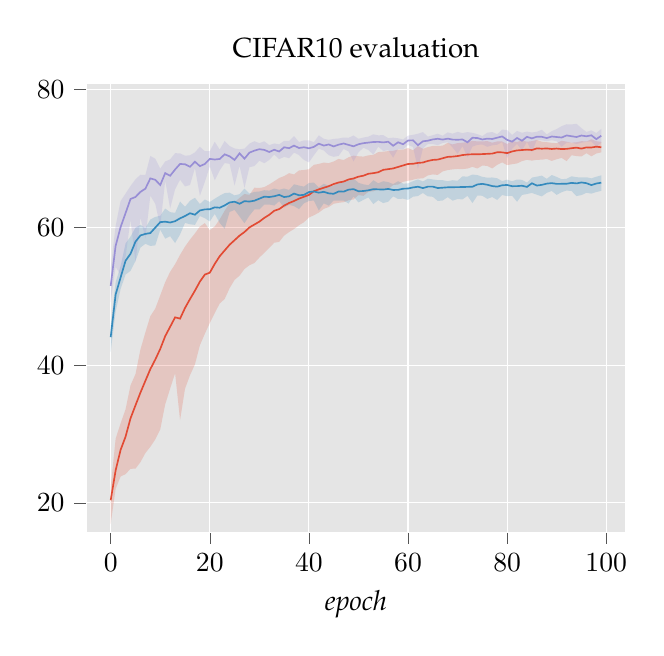
\begin{tikzpicture}

\definecolor{color0}{rgb}{0.886274509803922,0.290196078431373,0.2}
\definecolor{color1}{rgb}{0.203921568627451,0.541176470588235,0.741176470588235}
\definecolor{color2}{rgb}{0.596078431372549,0.556862745098039,0.835294117647059}

\begin{axis}[
axis background/.style={fill=white!89.8039215686275!black},
axis line style={white},
legend cell align={left},
legend style={fill opacity=0.8, draw opacity=1, text opacity=1, at={(0.97,0.03)}, anchor=south east, draw=white!80!black, fill=white!89.8039215686275!black},
log basis y={10},
tick align=outside,
tick pos=left,
title={CIFAR10 evaluation},
x grid style={white},
xlabel={\textit{epoch}},
xmajorgrids,
xmin=-4.95, xmax=103.95,
xtick style={color=white!33.3333333333333!black},
y grid style={white},
ymajorgrids,
ymin=15.7517645561491, ymax=80.8079673084566,
%ymode=log,
ytick style={color=white!33.3333333333333!black}
]
\path [fill=color0, fill opacity=0.2, very thin]
(axis cs:0,22.2756)
--(axis cs:0,16.9671)
--(axis cs:1,22.0553)
--(axis cs:2,23.8281)
--(axis cs:3,24.1787)
--(axis cs:4,24.9499)
--(axis cs:5,24.97)
--(axis cs:6,25.9115)
--(axis cs:7,27.2336)
--(axis cs:8,28.145)
--(axis cs:9,29.2167)
--(axis cs:10,30.6791)
--(axis cs:11,34.2949)
--(axis cs:12,36.5986)
--(axis cs:13,38.8321)
--(axis cs:14,32.0112)
--(axis cs:15,36.5785)
--(axis cs:16,38.5116)
--(axis cs:17,40.1042)
--(axis cs:18,42.8786)
--(axis cs:19,44.5413)
--(axis cs:20,46.1038)
--(axis cs:21,47.5561)
--(axis cs:22,48.9383)
--(axis cs:23,49.5893)
--(axis cs:24,51.1619)
--(axis cs:25,52.3638)
--(axis cs:26,52.9748)
--(axis cs:27,53.9463)
--(axis cs:28,54.4872)
--(axis cs:29,54.8177)
--(axis cs:30,55.599)
--(axis cs:31,56.3001)
--(axis cs:32,57.0112)
--(axis cs:33,57.7524)
--(axis cs:34,57.8826)
--(axis cs:35,58.7841)
--(axis cs:36,59.3049)
--(axis cs:37,59.7456)
--(axis cs:38,60.2965)
--(axis cs:39,60.7272)
--(axis cs:40,61.4183)
--(axis cs:41,61.7388)
--(axis cs:42,62.1294)
--(axis cs:43,62.6703)
--(axis cs:44,62.9307)
--(axis cs:45,63.4115)
--(axis cs:46,63.5517)
--(axis cs:47,63.6318)
--(axis cs:48,63.9223)
--(axis cs:49,64.0325)
--(axis cs:50,64.6735)
--(axis cs:51,64.5633)
--(axis cs:52,65.1542)
--(axis cs:53,65.2244)
--(axis cs:54,65.5349)
--(axis cs:55,65.5749)
--(axis cs:56,65.5449)
--(axis cs:57,66.1258)
--(axis cs:58,66.2059)
--(axis cs:59,66.5966)
--(axis cs:60,66.7368)
--(axis cs:61,66.897)
--(axis cs:62,67.0673)
--(axis cs:63,67.0873)
--(axis cs:64,67.528)
--(axis cs:65,67.6683)
--(axis cs:66,67.5982)
--(axis cs:67,68.109)
--(axis cs:68,68.2993)
--(axis cs:69,68.3994)
--(axis cs:70,68.4595)
--(axis cs:71,68.4395)
--(axis cs:72,68.5196)
--(axis cs:73,68.77)
--(axis cs:74,68.5296)
--(axis cs:75,68.9603)
--(axis cs:76,68.9002)
--(axis cs:77,68.5397)
--(axis cs:78,69.0605)
--(axis cs:79,69.4111)
--(axis cs:80,69.0204)
--(axis cs:81,69.1506)
--(axis cs:82,69.2608)
--(axis cs:83,69.6014)
--(axis cs:84,69.7917)
--(axis cs:85,69.6715)
--(axis cs:86,69.7917)
--(axis cs:87,69.8017)
--(axis cs:88,69.9119)
--(axis cs:89,69.6314)
--(axis cs:90,69.8718)
--(axis cs:91,70.0621)
--(axis cs:92,69.6014)
--(axis cs:93,70.4527)
--(axis cs:94,70.3325)
--(axis cs:95,70.2724)
--(axis cs:96,70.7532)
--(axis cs:97,70.3025)
--(axis cs:98,70.7031)
--(axis cs:99,70.8734)
--(axis cs:99,72.3958)
--(axis cs:99,72.3958)
--(axis cs:98,72.486)
--(axis cs:97,72.7764)
--(axis cs:96,72.4459)
--(axis cs:95,72.496)
--(axis cs:94,72.3357)
--(axis cs:93,72.2756)
--(axis cs:92,72.4159)
--(axis cs:91,72.5561)
--(axis cs:90,72.2055)
--(axis cs:89,72.2556)
--(axis cs:88,72.3458)
--(axis cs:87,72.4159)
--(axis cs:86,72.6763)
--(axis cs:85,72.496)
--(axis cs:84,72.4058)
--(axis cs:83,72.6262)
--(axis cs:82,72.3658)
--(axis cs:81,72.526)
--(axis cs:80,72.0753)
--(axis cs:79,72.4459)
--(axis cs:78,72.4559)
--(axis cs:77,72.2756)
--(axis cs:76,72.506)
--(axis cs:75,72.4559)
--(axis cs:74,72.4659)
--(axis cs:73,72.526)
--(axis cs:72,72.3658)
--(axis cs:71,72.2756)
--(axis cs:70,72.2155)
--(axis cs:69,72.0252)
--(axis cs:68,72.2456)
--(axis cs:67,71.845)
--(axis cs:66,71.7949)
--(axis cs:65,71.8049)
--(axis cs:64,71.6346)
--(axis cs:63,71.3842)
--(axis cs:62,71.7748)
--(axis cs:61,71.1739)
--(axis cs:60,71.5044)
--(axis cs:59,71.254)
--(axis cs:58,71.274)
--(axis cs:57,71.0938)
--(axis cs:56,71.0537)
--(axis cs:55,70.9635)
--(axis cs:54,70.9135)
--(axis cs:53,70.5028)
--(axis cs:52,70.4327)
--(axis cs:51,70.2524)
--(axis cs:50,70.3025)
--(axis cs:49,70.3926)
--(axis cs:48,70.1522)
--(axis cs:47,69.7516)
--(axis cs:46,69.9219)
--(axis cs:45,69.5513)
--(axis cs:44,69.3009)
--(axis cs:43,69.391)
--(axis cs:42,69.1907)
--(axis cs:41,69.0605)
--(axis cs:40,68.4195)
--(axis cs:39,68.3093)
--(axis cs:38,68.2492)
--(axis cs:37,67.6683)
--(axis cs:36,67.8486)
--(axis cs:35,67.4279)
--(axis cs:34,67.1474)
--(axis cs:33,66.6767)
--(axis cs:32,66.2159)
--(axis cs:31,65.8353)
--(axis cs:30,65.6951)
--(axis cs:29,65.7452)
--(axis cs:28,64.6935)
--(axis cs:27,64.8337)
--(axis cs:26,64.2628)
--(axis cs:25,63.6218)
--(axis cs:24,63.4816)
--(axis cs:23,62.3998)
--(axis cs:22,61.1378)
--(axis cs:21,60.1162)
--(axis cs:20,59.5753)
--(axis cs:19,60.607)
--(axis cs:18,60.1062)
--(axis cs:17,59.1046)
--(axis cs:16,58.2031)
--(axis cs:15,57.1915)
--(axis cs:14,55.9996)
--(axis cs:13,54.6474)
--(axis cs:12,53.5357)
--(axis cs:11,52.0333)
--(axis cs:10,50.1102)
--(axis cs:9,48.2071)
--(axis cs:8,47.0954)
--(axis cs:7,44.7416)
--(axis cs:6,42.2476)
--(axis cs:5,38.6819)
--(axis cs:4,37.0593)
--(axis cs:3,33.5737)
--(axis cs:2,31.5405)
--(axis cs:1,29.3269)
--(axis cs:0,22.2756)
--cycle;

\path [fill=color1, fill opacity=0.2, very thin]
(axis cs:0,45.7278)
--(axis cs:0,41.9205)
--(axis cs:1,47.765)
--(axis cs:2,51.0384)
--(axis cs:3,53.1349)
--(axis cs:4,53.6689)
--(axis cs:5,55.1028)
--(axis cs:6,57.051)
--(axis cs:7,57.6048)
--(axis cs:8,57.2884)
--(axis cs:9,57.3675)
--(axis cs:10,59.6519)
--(axis cs:11,58.3366)
--(axis cs:12,58.6926)
--(axis cs:13,57.7136)
--(axis cs:14,58.9498)
--(axis cs:15,60.6309)
--(axis cs:16,60.4331)
--(axis cs:17,60.3441)
--(axis cs:18,61.6297)
--(axis cs:19,61.3133)
--(axis cs:20,60.8386)
--(axis cs:21,61.9363)
--(axis cs:22,60.621)
--(axis cs:23,59.7805)
--(axis cs:24,62.2231)
--(axis cs:25,62.5198)
--(axis cs:26,61.5605)
--(axis cs:27,60.5815)
--(axis cs:28,61.6891)
--(axis cs:29,62.5791)
--(axis cs:30,62.5791)
--(axis cs:31,63.2812)
--(axis cs:32,63.301)
--(axis cs:33,63.1527)
--(axis cs:34,63.7757)
--(axis cs:35,62.8659)
--(axis cs:36,63.2615)
--(axis cs:37,63.0637)
--(axis cs:38,62.6385)
--(axis cs:39,63.4691)
--(axis cs:40,63.8153)
--(axis cs:41,63.8746)
--(axis cs:42,62.4308)
--(axis cs:43,63.4691)
--(axis cs:44,63.1428)
--(axis cs:45,63.8845)
--(axis cs:46,63.8647)
--(axis cs:47,63.8647)
--(axis cs:48,63.4395)
--(axis cs:49,64.468)
--(axis cs:50,63.5977)
--(axis cs:51,63.9735)
--(axis cs:52,64.3295)
--(axis cs:53,63.3604)
--(axis cs:54,63.924)
--(axis cs:55,63.5087)
--(axis cs:56,63.7065)
--(axis cs:57,64.4877)
--(axis cs:58,64.1021)
--(axis cs:59,64.1515)
--(axis cs:60,63.9735)
--(axis cs:61,64.4284)
--(axis cs:62,64.5372)
--(axis cs:63,64.9723)
--(axis cs:64,64.4877)
--(axis cs:65,64.4185)
--(axis cs:66,63.8153)
--(axis cs:67,63.8845)
--(axis cs:68,64.3691)
--(axis cs:69,63.8647)
--(axis cs:70,64.0922)
--(axis cs:71,64.0427)
--(axis cs:72,64.557)
--(axis cs:73,63.5186)
--(axis cs:74,64.6064)
--(axis cs:75,64.5668)
--(axis cs:76,64.1218)
--(axis cs:77,64.3888)
--(axis cs:78,63.9537)
--(axis cs:79,64.6756)
--(axis cs:80,64.5174)
--(axis cs:81,64.5767)
--(axis cs:82,63.6966)
--(axis cs:83,64.6855)
--(axis cs:84,64.824)
--(axis cs:85,64.9822)
--(axis cs:86,64.7251)
--(axis cs:87,64.4779)
--(axis cs:88,64.9921)
--(axis cs:89,65.269)
--(axis cs:90,64.6954)
--(axis cs:91,65.091)
--(axis cs:92,65.3283)
--(axis cs:93,65.2591)
--(axis cs:94,64.5273)
--(axis cs:95,64.6657)
--(axis cs:96,65.002)
--(axis cs:97,64.8833)
--(axis cs:98,65.1108)
--(axis cs:99,65.2888)
--(axis cs:99,67.5336)
--(axis cs:99,67.5336)
--(axis cs:98,67.3358)
--(axis cs:97,67.0985)
--(axis cs:96,67.2567)
--(axis cs:95,67.2271)
--(axis cs:94,67.2666)
--(axis cs:93,67.3952)
--(axis cs:92,67.0392)
--(axis cs:91,66.9699)
--(axis cs:90,67.3062)
--(axis cs:89,67.5831)
--(axis cs:88,67.0293)
--(axis cs:87,67.4941)
--(axis cs:86,67.3457)
--(axis cs:85,67.2073)
--(axis cs:84,66.4854)
--(axis cs:83,66.8809)
--(axis cs:82,66.9304)
--(axis cs:81,66.6733)
--(axis cs:80,66.9106)
--(axis cs:79,66.7029)
--(axis cs:78,67.1084)
--(axis cs:77,67.2271)
--(axis cs:76,67.1974)
--(axis cs:75,67.3161)
--(axis cs:74,67.5732)
--(axis cs:73,67.6523)
--(axis cs:72,67.3358)
--(axis cs:71,67.3952)
--(axis cs:70,66.7524)
--(axis cs:69,66.8315)
--(axis cs:68,66.6832)
--(axis cs:67,66.8315)
--(axis cs:66,66.8414)
--(axis cs:65,66.9403)
--(axis cs:64,67.049)
--(axis cs:63,66.6535)
--(axis cs:62,66.9502)
--(axis cs:61,66.6832)
--(axis cs:60,66.3667)
--(axis cs:59,66.337)
--(axis cs:58,66.6832)
--(axis cs:57,66.2678)
--(axis cs:56,66.5546)
--(axis cs:55,66.6832)
--(axis cs:54,66.3766)
--(axis cs:53,66.8315)
--(axis cs:52,66.1096)
--(axis cs:51,66.2282)
--(axis cs:50,66.4557)
--(axis cs:49,67.0985)
--(axis cs:48,66.7326)
--(axis cs:47,66.6337)
--(axis cs:46,66.4755)
--(axis cs:45,66.0502)
--(axis cs:44,66.0206)
--(axis cs:43,66.3172)
--(axis cs:42,65.7832)
--(axis cs:41,66.4854)
--(axis cs:40,66.426)
--(axis cs:39,65.9019)
--(axis cs:38,66.0502)
--(axis cs:37,66.2381)
--(axis cs:36,65.4173)
--(axis cs:35,65.625)
--(axis cs:34,65.4371)
--(axis cs:33,65.625)
--(axis cs:32,65.3184)
--(axis cs:31,65.3778)
--(axis cs:30,65.1899)
--(axis cs:29,65.1305)
--(axis cs:28,64.8932)
--(axis cs:27,65.625)
--(axis cs:26,64.8042)
--(axis cs:25,64.6262)
--(axis cs:24,65.0218)
--(axis cs:23,64.9624)
--(axis cs:22,64.5866)
--(axis cs:21,64.1416)
--(axis cs:20,63.6669)
--(axis cs:19,64.0328)
--(axis cs:18,63.3703)
--(axis cs:17,64.2801)
--(axis cs:16,63.8449)
--(axis cs:15,62.9747)
--(axis cs:14,63.7362)
--(axis cs:13,62.0945)
--(axis cs:12,62.1934)
--(axis cs:11,62.7176)
--(axis cs:10,61.6693)
--(axis cs:9,61.5012)
--(axis cs:8,61.1254)
--(axis cs:7,59.8794)
--(axis cs:6,60.3639)
--(axis cs:5,59.9288)
--(axis cs:4,58.6432)
--(axis cs:3,57.6543)
--(axis cs:2,54.3809)
--(axis cs:1,52.0372)
--(axis cs:0,45.7278)
--cycle;

\path [fill=color2, fill opacity=0.2, very thin]
(axis cs:0,54.153481)
--(axis cs:0,49.129747)
--(axis cs:1,54.252373)
--(axis cs:2,53.065665)
--(axis cs:3,55.676424)
--(axis cs:4,61.115506)
--(axis cs:5,54.924842)
--(axis cs:6,61.382516)
--(axis cs:7,58.356408)
--(axis cs:8,64.576741)
--(axis cs:9,63.399921)
--(axis cs:10,60.116693)
--(axis cs:11,66.742484)
--(axis cs:12,62.717563)
--(axis cs:13,65.516218)
--(axis cs:14,66.900712)
--(axis cs:15,65.921677)
--(axis cs:16,66.129351)
--(axis cs:17,68.571994)
--(axis cs:18,64.566851)
--(axis cs:19,66.574367)
--(axis cs:20,68.819225)
--(axis cs:21,66.821598)
--(axis cs:22,68.255538)
--(axis cs:23,69.323576)
--(axis cs:24,69.195016)
--(axis cs:25,66.040348)
--(axis cs:26,68.918117)
--(axis cs:27,65.704114)
--(axis cs:28,68.710443)
--(axis cs:29,68.87856)
--(axis cs:30,69.649921)
--(axis cs:31,69.293908)
--(axis cs:32,69.768592)
--(axis cs:33,70.549842)
--(axis cs:34,69.877373)
--(axis cs:35,70.213608)
--(axis cs:36,70.015823)
--(axis cs:37,70.826741)
--(axis cs:38,70.480617)
--(axis cs:39,69.768592)
--(axis cs:40,69.412579)
--(axis cs:41,70.44106)
--(axis cs:42,71.400316)
--(axis cs:43,71.143196)
--(axis cs:44,70.460839)
--(axis cs:45,70.223497)
--(axis cs:46,70.352057)
--(axis cs:47,71.370649)
--(axis cs:48,70.994858)
--(axis cs:49,69.541139)
--(axis cs:50,70.866297)
--(axis cs:51,71.538766)
--(axis cs:52,71.212421)
--(axis cs:53,70.530063)
--(axis cs:54,71.696994)
--(axis cs:55,71.064082)
--(axis cs:56,71.192642)
--(axis cs:57,70.094937)
--(axis cs:58,71.380538)
--(axis cs:59,71.301424)
--(axis cs:60,71.934335)
--(axis cs:61,71.657437)
--(axis cs:62,68.453323)
--(axis cs:63,71.420095)
--(axis cs:64,72.082674)
--(axis cs:65,72.072785)
--(axis cs:66,71.914557)
--(axis cs:67,72.221123)
--(axis cs:68,72.349684)
--(axis cs:69,71.568434)
--(axis cs:70,70.658623)
--(axis cs:71,71.74644)
--(axis cs:72,70.154272)
--(axis cs:73,71.716772)
--(axis cs:74,71.954114)
--(axis cs:75,72.013449)
--(axis cs:76,71.677215)
--(axis cs:77,71.894778)
--(axis cs:78,71.973892)
--(axis cs:79,72.359573)
--(axis cs:80,70.035601)
--(axis cs:81,71.400316)
--(axis cs:82,72.102453)
--(axis cs:83,71.123418)
--(axis cs:84,72.39913)
--(axis cs:85,70.935522)
--(axis cs:86,72.676028)
--(axis cs:87,72.606804)
--(axis cs:88,72.478244)
--(axis cs:89,72.626582)
--(axis cs:90,72.478244)
--(axis cs:91,71.677215)
--(axis cs:92,72.290348)
--(axis cs:93,72.300237)
--(axis cs:94,72.082674)
--(axis cs:95,72.27057)
--(axis cs:96,72.409019)
--(axis cs:97,72.458465)
--(axis cs:98,71.706883)
--(axis cs:99,72.26068)
--(axis cs:99,74.278085)
--(axis cs:99,74.278085)
--(axis cs:98,73.684731)
--(axis cs:97,74.060522)
--(axis cs:96,73.83307)
--(axis cs:95,74.386867)
--(axis cs:94,75.019778)
--(axis cs:93,74.920886)
--(axis cs:92,74.950554)
--(axis cs:91,74.673655)
--(axis cs:90,74.258307)
--(axis cs:89,73.951741)
--(axis cs:88,73.486946)
--(axis cs:87,74.149525)
--(axis cs:86,73.862737)
--(axis cs:85,73.753956)
--(axis cs:84,73.882516)
--(axis cs:83,73.714399)
--(axis cs:82,73.981408)
--(axis cs:81,73.397943)
--(axis cs:80,74.109968)
--(axis cs:79,74.179193)
--(axis cs:78,73.506725)
--(axis cs:77,73.82318)
--(axis cs:76,73.724288)
--(axis cs:75,73.239715)
--(axis cs:74,73.516614)
--(axis cs:73,73.704509)
--(axis cs:72,73.813291)
--(axis cs:71,73.664953)
--(axis cs:70,73.842959)
--(axis cs:69,73.585839)
--(axis cs:68,73.773734)
--(axis cs:67,73.289161)
--(axis cs:66,73.575949)
--(axis cs:65,73.358386)
--(axis cs:64,73.160601)
--(axis cs:63,73.813291)
--(axis cs:62,73.575949)
--(axis cs:61,73.407832)
--(axis cs:60,73.299051)
--(axis cs:59,72.735364)
--(axis cs:58,72.91337)
--(axis cs:57,73.002373)
--(axis cs:56,72.933149)
--(axis cs:55,73.378165)
--(axis cs:54,73.338608)
--(axis cs:53,73.486946)
--(axis cs:52,73.150712)
--(axis cs:51,73.022152)
--(axis cs:50,72.844146)
--(axis cs:49,73.318829)
--(axis cs:48,72.982595)
--(axis cs:47,73.022152)
--(axis cs:46,72.883703)
--(axis cs:45,72.824367)
--(axis cs:44,72.685918)
--(axis cs:43,72.844146)
--(axis cs:42,73.338608)
--(axis cs:41,72.349684)
--(axis cs:40,72.616693)
--(axis cs:39,72.626582)
--(axis cs:38,72.369462)
--(axis cs:37,73.239715)
--(axis cs:36,72.52769)
--(axis cs:35,72.547468)
--(axis cs:34,72.033228)
--(axis cs:33,72.161788)
--(axis cs:32,71.924446)
--(axis cs:31,72.478244)
--(axis cs:30,72.201345)
--(axis cs:29,72.488133)
--(axis cs:28,72.142009)
--(axis cs:27,71.420095)
--(axis cs:26,71.311313)
--(axis cs:25,71.439873)
--(axis cs:24,71.795886)
--(axis cs:23,72.52769)
--(axis cs:22,71.281646)
--(axis cs:21,72.409019)
--(axis cs:20,71.044304)
--(axis cs:19,71.034415)
--(axis cs:18,71.687104)
--(axis cs:17,70.866297)
--(axis cs:16,70.450949)
--(axis cs:15,70.381725)
--(axis cs:14,70.727848)
--(axis cs:13,70.747627)
--(axis cs:12,69.857595)
--(axis cs:11,69.551028)
--(axis cs:10,68.502769)
--(axis cs:9,69.946598)
--(axis cs:8,70.352057)
--(axis cs:7,67.592959)
--(axis cs:6,67.622627)
--(axis cs:5,66.960047)
--(axis cs:4,65.990902)
--(axis cs:3,64.893196)
--(axis cs:2,63.815269)
--(axis cs:1,60.215585)
--(axis cs:0,54.153481)
--cycle;

\addplot [semithick, color0]
table {%
0 20.3896198272705
1 24.7235527038574
2 27.6973209381104
3 29.6133804321289
4 32.2686347961426
5 34.1556663513184
6 35.9986000061035
7 37.7153549194336
8 39.4130516052246
9 40.8022880554199
10 42.3437614440918
11 44.1957244873047
13 46.9310646057129
14 46.7427825927734
15 48.2922515869141
16 49.5753059387207
17 50.7982864379883
18 52.1123924255371
19 53.132022857666
20 53.4134674072266
21 54.6864967346191
22 55.8002662658691
24 57.4719657897949
26 58.7840576171875
27 59.3119049072266
28 59.9799652099609
30 60.8153076171875
31 61.360179901123
32 61.8129081726074
33 62.3918151855469
34 62.6311988830566
35 63.1410140991211
36 63.5236396789551
37 63.8120994567871
38 64.1576385498047
40 64.6895217895508
41 65.2303619384766
42 65.5038070678711
44 65.9635467529297
45 66.2730560302734
46 66.4983901977539
47 66.6316070556641
48 66.9350814819336
49 67.0803298950195
50 67.3437423706055
51 67.485969543457
52 67.7634201049805
53 67.8525772094727
54 67.9847717285156
55 68.3333206176758
57 68.5366668701172
60 69.184700012207
61 69.2127532958984
62 69.340934753418
63 69.3960418701172
64 69.6223831176758
65 69.7736358642578
66 69.8207244873047
68 70.2133483886719
69 70.2533874511719
70 70.3355331420898
71 70.4787521362305
72 70.5578842163086
73 70.5919418334961
74 70.5839157104492
77 70.6930999755859
78 70.8844375610352
79 70.8724136352539
80 70.7562103271484
81 71.0045700073242
82 71.1488418579102
84 71.265022277832
85 71.2139434814453
86 71.4463119506836
87 71.3992462158203
88 71.4373092651367
89 71.3601760864258
90 71.421272277832
91 71.3481521606445
92 71.377197265625
94 71.5594787597656
95 71.4132537841797
96 71.5885391235352
97 71.5755310058594
98 71.6977233886719
99 71.6085662841797
};
%\addlegendentry{cudnn}
\addplot [semithick, color1]
table {%
0 44.0516204833984
1 50.2492065429688
2 52.7126274108887
3 55.1443901062012
4 56.1491165161133
5 57.9034729003906
6 58.8113021850586
7 59.0387763977051
8 59.1574554443359
10 60.7456359863281
11 60.8089485168457
12 60.6892547607422
13 60.8831024169922
14 61.2964782714844
15 61.6297492980957
16 62.0361862182617
17 61.8235778808594
18 62.4376792907715
19 62.5979080200195
20 62.6107597351074
21 62.8916244506836
22 62.8382186889648
23 63.1714935302734
24 63.6026573181152
25 63.7124252319336
26 63.4157447814941
27 63.7885627746582
28 63.7302131652832
29 63.8558158874512
31 64.4442367553711
32 64.3858871459961
33 64.4986190795898
34 64.7023239135742
35 64.384880065918
36 64.4887237548828
37 64.8882522583008
38 64.6390609741211
39 64.7013626098633
40 65.1067886352539
41 65.1928405761719
42 65.018798828125
43 65.1433868408203
44 64.9199142456055
45 64.8565979003906
46 65.1968154907227
47 65.1730575561523
48 65.4549026489258
49 65.5369873046875
50 65.2264404296875
51 65.2600936889648
52 65.3639450073242
53 65.5271148681641
55 65.4687576293945
56 65.5656661987305
57 65.4153289794922
58 65.4272003173828
59 65.5943450927734
60 65.6220397949219
61 65.7792816162109
62 65.8831100463867
63 65.6873016357422
64 65.8919906616211
65 65.8989410400391
66 65.6912460327148
68 65.7990570068359
71 65.8386001586914
73 65.8851013183594
74 66.2143783569336
75 66.2994537353516
76 66.1688995361328
77 65.97705078125
78 65.8939971923828
79 66.0967102050781
80 66.1382675170898
81 65.9612274169922
82 65.9701385498047
83 66.0255126953125
84 65.8593902587891
85 66.385498046875
86 66.0532150268555
87 66.1550827026367
88 66.3340606689453
89 66.4082260131836
90 66.2965087890625
92 66.3123016357422
93 66.4428482055664
94 66.3647308349609
95 66.503173828125
96 66.3993301391602
97 66.1224365234375
98 66.3479156494141
99 66.4685516357422
};
%\addlegendentry{libtorch}
\addplot [semithick, color2]
table {%
0 51.5002021789551
1 57.3081474304199
2 60.0267066955566
3 62.0520248413086
4 64.1020660400391
5 64.394775390625
6 65.1335144042969
7 65.5992965698242
8 67.0895919799805
9 66.8858795166016
10 66.1303329467773
11 67.8550338745117
12 67.4782485961914
13 68.3860855102539
14 69.1880950927734
15 69.1406173706055
16 68.7737350463867
17 69.5174102783203
18 68.8686599731445
19 69.1821517944336
20 69.9248504638672
21 69.8308868408203
22 69.911994934082
23 70.5824661254883
24 70.2966766357422
25 69.7725448608398
26 70.7248916625977
27 69.9554901123047
28 70.8316879272461
29 71.1194610595703
30 71.3281173706055
31 71.2282333374023
32 70.9206924438477
33 71.2470245361328
34 70.9968338012695
35 71.6040267944336
36 71.4784469604492
37 71.8482971191406
38 71.5002059936523
39 71.6139297485352
40 71.4586715698242
41 71.6663360595703
42 72.128173828125
43 71.856201171875
44 72.0124664306641
45 71.7306137084961
46 71.9887313842773
47 72.1588287353516
49 71.7464447021484
50 72.0470657348633
51 72.2023391723633
53 72.372428894043
54 72.3951721191406
55 72.3160705566406
56 72.4129638671875
57 71.8334655761719
58 72.3318939208984
59 72.0440979003906
60 72.5929489135742
61 72.6176834106445
62 71.9155349731445
63 72.4723205566406
64 72.5632858276367
65 72.7452621459961
66 72.842170715332
67 72.7225036621094
68 72.861946105957
69 72.724479675293
70 72.6987762451172
71 72.7412872314453
72 72.3299026489258
73 72.9895172119141
74 72.9469985961914
75 72.7403106689453
76 72.8609466552734
77 72.8125076293945
79 73.1843414306641
80 72.6790008544922
81 72.4228591918945
82 72.9578704833984
83 72.5573501586914
84 73.1269683837891
85 72.8965606689453
86 73.1388549804688
87 73.125
88 72.9410705566406
89 73.1714859008789
91 73.0221633911133
92 73.3247680664062
94 73.0973052978516
95 73.3119125366211
96 73.203125
97 73.3445358276367
98 72.7877655029297
99 73.2852096557617
};
%\addlegendentry{pytorch}
\end{axis}

\end{tikzpicture}

        \end{adjustbox}
      \end{subfigure}
      \\[1ex]
      \begin{subfigure}{0.24\linewidth}
        \centering
        \begin{adjustbox}{width=\textwidth}
          % This file was created by tikzplotlib v0.9.5.
\begin{tikzpicture}





\begin{axis}[
axis background/.style={fill=white!89.8039215686275!black},
axis line style={white},
legend cell align={left},
legend style={fill opacity=0.8, draw opacity=1, text opacity=1, at={(0.97,0.03)}, anchor=south east, draw=white!80!black, fill=white!89.8039215686275!black},
log basis y={10},
tick align=outside,
tick pos=left,
title={STL10 training},
x grid style={white},
xlabel={time},
xmajorgrids,
xmin=-5.19760163, xmax=135.38068523,
xtick style={color=white!33.3333333333333!black},
y grid style={white},
ylabel={accuracy},
ymajorgrids,
ymin=9.14280358979306, ymax=109.315558819346,
%ymode=log,
ytick style={color=white!33.3333333333333!black}
]
\path [fill=cudnn, fill opacity=0.2, very thin]
(axis cs:1.8181475,13.919271)
--(axis cs:1.8181475,10.234375)
--(axis cs:3.1015922,11.341146)
--(axis cs:4.3881964,13.541667)
--(axis cs:5.6697498,14.817708)
--(axis cs:6.9567745,16.848959)
--(axis cs:8.2428672,17.942709)
--(axis cs:9.5269492,18.619791)
--(axis cs:10.8122282,18.333334)
--(axis cs:12.0991791,19.322916)
--(axis cs:13.3812914,19.166666)
--(axis cs:14.6654891,19.661459)
--(axis cs:15.9478969,20.195312)
--(axis cs:17.232328,21.354166)
--(axis cs:18.5146575,21.640625)
--(axis cs:19.8012213,21.744791)
--(axis cs:21.0840842,22.304688)
--(axis cs:22.3683458,22.591146)
--(axis cs:23.651952,22.708334)
--(axis cs:24.9376781,24.023438)
--(axis cs:26.2201795,24.505209)
--(axis cs:27.5038189,24.713541)
--(axis cs:28.7885163,24.973959)
--(axis cs:30.0761489,25.742188)
--(axis cs:31.358376,25.065104)
--(axis cs:32.6423435,26.210938)
--(axis cs:33.9274175,26.770834)
--(axis cs:35.2126796,26.692709)
--(axis cs:36.4976855,26.953125)
--(axis cs:37.7835537,28.190104)
--(axis cs:39.0670015,28.971354)
--(axis cs:40.3503277,30.039062)
--(axis cs:41.6357876,30.182291)
--(axis cs:42.9215691,30.598959)
--(axis cs:44.2048227,30.598959)
--(axis cs:45.490117,31.25)
--(axis cs:46.7742425,31.549479)
--(axis cs:48.0608687,31.744791)
--(axis cs:49.3439484,32.005207)
--(axis cs:50.628987,32.161457)
--(axis cs:51.9142668,32.5)
--(axis cs:53.1983139,33.320312)
--(axis cs:54.4834733,32.903645)
--(axis cs:55.7678699,33.815105)
--(axis cs:57.0510268,33.91927)
--(axis cs:58.3349453,34.270832)
--(axis cs:59.6192652,34.947918)
--(axis cs:60.9042402,35.01302)
--(axis cs:62.1854784,35.182293)
--(axis cs:63.4683535,35.833332)
--(axis cs:64.7523611,36.289062)
--(axis cs:66.0399125,35.651043)
--(axis cs:67.3233237,36.484375)
--(axis cs:68.6089274,37.33073)
--(axis cs:69.8913879,37.382812)
--(axis cs:71.1745869,37.942707)
--(axis cs:72.4576266,37.8125)
--(axis cs:73.7439566,39.0625)
--(axis cs:75.0281581,38.346355)
--(axis cs:76.3165164,38.320312)
--(axis cs:77.5979577,39.0625)
--(axis cs:78.8851048,39.192707)
--(axis cs:80.1680884,39.0625)
--(axis cs:81.4541719,39.192707)
--(axis cs:82.738797,39.973957)
--(axis cs:84.0242694,39.726562)
--(axis cs:85.3116352,39.934895)
--(axis cs:86.5965253,40.039062)
--(axis cs:87.8830559,40.182293)
--(axis cs:89.1684826,39.947918)
--(axis cs:90.451034,40.690105)
--(axis cs:91.7357714,41.132812)
--(axis cs:93.0172198,41.315105)
--(axis cs:94.3033933,40.742188)
--(axis cs:95.5860217,41.835938)
--(axis cs:96.8740081,41.041668)
--(axis cs:98.1589983,42.070312)
--(axis cs:99.4438364,41.5625)
--(axis cs:100.726415,41.835938)
--(axis cs:102.009401,42.005207)
--(axis cs:103.2938186,42.005207)
--(axis cs:104.5794376,41.653645)
--(axis cs:105.8616588,42.434895)
--(axis cs:107.1464607,42.851562)
--(axis cs:108.4291424,42.98177)
--(axis cs:109.7167975,43.307293)
--(axis cs:111.0016509,43.046875)
--(axis cs:112.2889483,42.5)
--(axis cs:113.5706432,43.76302)
--(axis cs:114.855097,43.059895)
--(axis cs:116.1407626,43.502605)
--(axis cs:117.4265288,43.463543)
--(axis cs:118.7118835,44.38802)
--(axis cs:119.9955895,43.463543)
--(axis cs:121.2795428,44.192707)
--(axis cs:122.567516,43.945312)
--(axis cs:123.8486356,44.440105)
--(axis cs:125.1355257,44.101562)
--(axis cs:126.4196376,44.38802)
--(axis cs:127.7084405,44.296875)
--(axis cs:128.9907631,43.802082)
--(axis cs:128.9907631,58.007812)
--(axis cs:128.9907631,58.007812)
--(axis cs:127.7084405,57.057293)
--(axis cs:126.4196376,57.382812)
--(axis cs:125.1355257,57.122395)
--(axis cs:123.8486356,56.744793)
--(axis cs:122.567516,57.070312)
--(axis cs:121.2795428,56.875)
--(axis cs:119.9955895,56.5625)
--(axis cs:118.7118835,56.328125)
--(axis cs:117.4265288,55.898438)
--(axis cs:116.1407626,55.755207)
--(axis cs:114.855097,55.885418)
--(axis cs:113.5706432,55.338543)
--(axis cs:112.2889483,55.14323)
--(axis cs:111.0016509,54.427082)
--(axis cs:109.7167975,55.351562)
--(axis cs:108.4291424,54.882812)
--(axis cs:107.1464607,54.609375)
--(axis cs:105.8616588,54.166668)
--(axis cs:104.5794376,53.91927)
--(axis cs:103.2938186,53.463543)
--(axis cs:102.009401,54.140625)
--(axis cs:100.726415,53.164062)
--(axis cs:99.4438364,53.515625)
--(axis cs:98.1589983,52.747395)
--(axis cs:96.8740081,53.815105)
--(axis cs:95.5860217,52.890625)
--(axis cs:94.3033933,52.382812)
--(axis cs:93.0172198,52.864582)
--(axis cs:91.7357714,52.35677)
--(axis cs:90.451034,51.54948)
--(axis cs:89.1684826,51.88802)
--(axis cs:87.8830559,51.23698)
--(axis cs:86.5965253,50.182293)
--(axis cs:85.3116352,51.54948)
--(axis cs:84.0242694,50.039062)
--(axis cs:82.738797,51.341145)
--(axis cs:81.4541719,50.208332)
--(axis cs:80.1680884,50.716145)
--(axis cs:78.8851048,50.833332)
--(axis cs:77.5979577,50.338543)
--(axis cs:76.3165164,49.83073)
--(axis cs:75.0281581,49.960938)
--(axis cs:73.7439566,49.51823)
--(axis cs:72.4576266,49.36198)
--(axis cs:71.1745869,49.140625)
--(axis cs:69.8913879,49.07552)
--(axis cs:68.6089274,47.65625)
--(axis cs:67.3233237,47.994793)
--(axis cs:66.0399125,48.046875)
--(axis cs:64.7523611,47.96875)
--(axis cs:63.4683535,47.447918)
--(axis cs:62.1854784,47.20052)
--(axis cs:60.9042402,46.666668)
--(axis cs:59.6192652,46.302082)
--(axis cs:58.3349453,46.57552)
--(axis cs:57.0510268,45.885418)
--(axis cs:55.7678699,46.028645)
--(axis cs:54.4834733,46.432293)
--(axis cs:53.1983139,46.223957)
--(axis cs:51.9142668,45.677082)
--(axis cs:50.628987,44.934895)
--(axis cs:49.3439484,45.234375)
--(axis cs:48.0608687,44.401043)
--(axis cs:46.7742425,43.89323)
--(axis cs:45.490117,43.932293)
--(axis cs:44.2048227,43.997395)
--(axis cs:42.9215691,43.320312)
--(axis cs:41.6357876,43.151043)
--(axis cs:40.3503277,43.216145)
--(axis cs:39.0670015,42.708332)
--(axis cs:37.7835537,41.471355)
--(axis cs:36.4976855,41.39323)
--(axis cs:35.2126796,41.119793)
--(axis cs:33.9274175,41.028645)
--(axis cs:32.6423435,41.119793)
--(axis cs:31.358376,40)
--(axis cs:30.0761489,39.23177)
--(axis cs:28.7885163,40.065105)
--(axis cs:27.5038189,38.984375)
--(axis cs:26.2201795,39.179688)
--(axis cs:24.9376781,39.04948)
--(axis cs:23.651952,38.007812)
--(axis cs:22.3683458,37.760418)
--(axis cs:21.0840842,38.177082)
--(axis cs:19.8012213,36.666668)
--(axis cs:18.5146575,36.067707)
--(axis cs:17.232328,35.833332)
--(axis cs:15.9478969,34.244793)
--(axis cs:14.6654891,34.739582)
--(axis cs:13.3812914,32.578125)
--(axis cs:12.0991791,32.682293)
--(axis cs:10.8122282,31.289062)
--(axis cs:9.5269492,30.546875)
--(axis cs:8.2428672,29.388021)
--(axis cs:6.9567745,27.851562)
--(axis cs:5.6697498,26.119791)
--(axis cs:4.3881964,23.997396)
--(axis cs:3.1015922,17.486979)
--(axis cs:1.8181475,13.919271)
--cycle;

\path [fill=libtorch, fill opacity=0.2, very thin]
(axis cs:1.2572434,16.328125)
--(axis cs:1.2572434,13.339844)
--(axis cs:2.5172312,19.179688)
--(axis cs:3.7711002,26.796875)
--(axis cs:5.022725,31.972656)
--(axis cs:6.2778645,37.636719)
--(axis cs:7.5325557,39.746094)
--(axis cs:8.7884026,45.800781)
--(axis cs:10.0442825,50.234375)
--(axis cs:11.3001487,52.519531)
--(axis cs:12.5558317,57.539062)
--(axis cs:13.813037,61.445312)
--(axis cs:15.0695192,66.230469)
--(axis cs:16.3259816,71.367188)
--(axis cs:17.581719,65.507812)
--(axis cs:18.8377473,71.992188)
--(axis cs:20.0918182,74.824219)
--(axis cs:21.3473531,79.0625)
--(axis cs:22.603765,75.722656)
--(axis cs:23.861623,81.503906)
--(axis cs:25.1170369,78.242188)
--(axis cs:26.3717957,81.738281)
--(axis cs:27.6281248,79.960938)
--(axis cs:28.8846523,81.289062)
--(axis cs:30.1416594,85.566406)
--(axis cs:31.3969638,88.222656)
--(axis cs:32.6534027,86.914062)
--(axis cs:33.9101459,84.609375)
--(axis cs:35.1660355,80.292969)
--(axis cs:36.422017,79.472656)
--(axis cs:37.6763219,85.644531)
--(axis cs:38.931803,87.011719)
--(axis cs:40.1894583,87.578125)
--(axis cs:41.446448,90.429688)
--(axis cs:42.7027211,89.960938)
--(axis cs:43.9562373,88.808594)
--(axis cs:45.2120456,87.734375)
--(axis cs:46.4665121,89.980469)
--(axis cs:47.7242048,87.851562)
--(axis cs:48.9775083,88.710938)
--(axis cs:50.2334429,91.933594)
--(axis cs:51.4900184,88.671875)
--(axis cs:52.745522,85.585938)
--(axis cs:53.9997774,89.394531)
--(axis cs:55.2561939,88.632812)
--(axis cs:56.5128563,91.757812)
--(axis cs:57.7700699,92.714844)
--(axis cs:59.0265381,92.148438)
--(axis cs:60.2807585,92.460938)
--(axis cs:61.5355289,92.421875)
--(axis cs:62.7895891,89.980469)
--(axis cs:64.0442244,91.679688)
--(axis cs:65.3006613,93.28125)
--(axis cs:66.5541206,90.742188)
--(axis cs:67.8099738,89.042969)
--(axis cs:69.0641438,93.085938)
--(axis cs:70.3209835,92.8125)
--(axis cs:71.5770803,93.847656)
--(axis cs:72.83228,93.671875)
--(axis cs:74.0878983,91.621094)
--(axis cs:75.3433888,87.265625)
--(axis cs:76.5951476,94.355469)
--(axis cs:77.8479253,93.183594)
--(axis cs:79.1027417,93.046875)
--(axis cs:80.3586953,94.550781)
--(axis cs:81.6110766,93.808594)
--(axis cs:82.866656,92.34375)
--(axis cs:84.122545,91.699219)
--(axis cs:85.378461,89.84375)
--(axis cs:86.6355466,93.691406)
--(axis cs:87.8884647,94.433594)
--(axis cs:89.1453755,94.433594)
--(axis cs:90.4002351,95.273438)
--(axis cs:91.6575148,93.828125)
--(axis cs:92.9107424,91.894531)
--(axis cs:94.1655439,93.378906)
--(axis cs:95.4185916,93.886719)
--(axis cs:96.6754833,92.03125)
--(axis cs:97.9307792,92.128906)
--(axis cs:99.1860832,90.566406)
--(axis cs:100.4418415,91.777344)
--(axis cs:101.6954069,93.4375)
--(axis cs:102.9511175,91.992188)
--(axis cs:104.2052924,91.777344)
--(axis cs:105.4607916,94.296875)
--(axis cs:106.7130088,94.335938)
--(axis cs:107.9684443,92.421875)
--(axis cs:109.2243049,93.320312)
--(axis cs:110.4802955,95.234375)
--(axis cs:111.7352181,93.554688)
--(axis cs:112.9894661,93.476562)
--(axis cs:114.2429628,93.378906)
--(axis cs:115.4969641,90.9375)
--(axis cs:116.7545363,94.316406)
--(axis cs:118.0090586,94.414062)
--(axis cs:119.2647401,94.042969)
--(axis cs:120.5219174,93.886719)
--(axis cs:121.7776013,93.378906)
--(axis cs:123.0304152,92.96875)
--(axis cs:124.2862077,92.65625)
--(axis cs:125.5408108,94.355469)
--(axis cs:125.5408108,97.324219)
--(axis cs:125.5408108,97.324219)
--(axis cs:124.2862077,97.597656)
--(axis cs:123.0304152,97.5)
--(axis cs:121.7776013,97.402344)
--(axis cs:120.5219174,96.445312)
--(axis cs:119.2647401,97.558594)
--(axis cs:118.0090586,97.636719)
--(axis cs:116.7545363,97.578125)
--(axis cs:115.4969641,97.207031)
--(axis cs:114.2429628,97.617188)
--(axis cs:112.9894661,97.65625)
--(axis cs:111.7352181,97.65625)
--(axis cs:110.4802955,97.65625)
--(axis cs:109.2243049,97.636719)
--(axis cs:107.9684443,97.539062)
--(axis cs:106.7130088,97.363281)
--(axis cs:105.4607916,97.578125)
--(axis cs:104.2052924,97.519531)
--(axis cs:102.9511175,97.363281)
--(axis cs:101.6954069,97.519531)
--(axis cs:100.4418415,97.65625)
--(axis cs:99.1860832,97.382812)
--(axis cs:97.9307792,97.441406)
--(axis cs:96.6754833,97.558594)
--(axis cs:95.4185916,97.5)
--(axis cs:94.1655439,97.324219)
--(axis cs:92.9107424,97.402344)
--(axis cs:91.6575148,97.558594)
--(axis cs:90.4002351,97.402344)
--(axis cs:89.1453755,97.363281)
--(axis cs:87.8884647,97.519531)
--(axis cs:86.6355466,97.519531)
--(axis cs:85.378461,97.441406)
--(axis cs:84.122545,97.109375)
--(axis cs:82.866656,97.441406)
--(axis cs:81.6110766,97.363281)
--(axis cs:80.3586953,97.578125)
--(axis cs:79.1027417,96.972656)
--(axis cs:77.8479253,97.480469)
--(axis cs:76.5951476,97.246094)
--(axis cs:75.3433888,97.011719)
--(axis cs:74.0878983,97.558594)
--(axis cs:72.83228,97.519531)
--(axis cs:71.5770803,97.363281)
--(axis cs:70.3209835,97.441406)
--(axis cs:69.0641438,96.816406)
--(axis cs:67.8099738,97.519531)
--(axis cs:66.5541206,97.617188)
--(axis cs:65.3006613,97.519531)
--(axis cs:64.0442244,97.226562)
--(axis cs:62.7895891,97.304688)
--(axis cs:61.5355289,97.285156)
--(axis cs:60.2807585,97.167969)
--(axis cs:59.0265381,97.070312)
--(axis cs:57.7700699,97.148438)
--(axis cs:56.5128563,96.953125)
--(axis cs:55.2561939,97.1875)
--(axis cs:53.9997774,96.914062)
--(axis cs:52.745522,97.265625)
--(axis cs:51.4900184,97.460938)
--(axis cs:50.2334429,97.421875)
--(axis cs:48.9775083,96.386719)
--(axis cs:47.7242048,96.445312)
--(axis cs:46.4665121,97.265625)
--(axis cs:45.2120456,97.128906)
--(axis cs:43.9562373,96.601562)
--(axis cs:42.7027211,96.914062)
--(axis cs:41.446448,97.128906)
--(axis cs:40.1894583,97.285156)
--(axis cs:38.931803,97.167969)
--(axis cs:37.6763219,94.84375)
--(axis cs:36.422017,94.84375)
--(axis cs:35.1660355,95.976562)
--(axis cs:33.9101459,96.699219)
--(axis cs:32.6534027,95.878906)
--(axis cs:31.3969638,96.113281)
--(axis cs:30.1416594,95.410156)
--(axis cs:28.8846523,95.351562)
--(axis cs:27.6281248,93.261719)
--(axis cs:26.3717957,90.019531)
--(axis cs:25.1170369,93.730469)
--(axis cs:23.861623,91.699219)
--(axis cs:22.603765,90.800781)
--(axis cs:21.3473531,86.210938)
--(axis cs:20.0918182,86.992188)
--(axis cs:18.8377473,82.324219)
--(axis cs:17.581719,78.886719)
--(axis cs:16.3259816,76.875)
--(axis cs:15.0695192,75.800781)
--(axis cs:13.813037,69.609375)
--(axis cs:12.5558317,64.296875)
--(axis cs:11.3001487,58.652344)
--(axis cs:10.0442825,54.84375)
--(axis cs:8.7884026,50.488281)
--(axis cs:7.5325557,45.039062)
--(axis cs:6.2778645,40.253906)
--(axis cs:5.022725,36.816406)
--(axis cs:3.7711002,31.386719)
--(axis cs:2.5172312,24.140625)
--(axis cs:1.2572434,16.328125)
--cycle;

\path [fill=pytorch, fill opacity=0.2, very thin]
(axis cs:1.1923205,19.023438)
--(axis cs:1.1923205,17.03125)
--(axis cs:2.3809789,29.433594)
--(axis cs:3.5703207,40.292969)
--(axis cs:4.7594273,47.558594)
--(axis cs:5.9488041,57.207031)
--(axis cs:7.1392454,55.625)
--(axis cs:8.3290476,62.714844)
--(axis cs:9.5191099,68.359375)
--(axis cs:10.7087473,67.792969)
--(axis cs:11.8987529,68.359375)
--(axis cs:13.0881655,74.726562)
--(axis cs:14.2777552,79.277344)
--(axis cs:15.4673408,80.566406)
--(axis cs:16.6568362,85.019531)
--(axis cs:17.8460565,81.582031)
--(axis cs:19.0356783,83.691406)
--(axis cs:20.2255283,82.734375)
--(axis cs:21.4154439,74.921875)
--(axis cs:22.6050104,77.226562)
--(axis cs:23.7949036,81.972656)
--(axis cs:24.9849541,82.597656)
--(axis cs:26.1750076,84.296875)
--(axis cs:27.3654415,87.089844)
--(axis cs:28.5549483,85.957031)
--(axis cs:29.7453015,87.011719)
--(axis cs:30.934922,90.527344)
--(axis cs:32.1249991,80.605469)
--(axis cs:33.3145505,88.867188)
--(axis cs:34.5045081,82.011719)
--(axis cs:35.6935889,89.023438)
--(axis cs:36.8828063,88.378906)
--(axis cs:38.0722721,86.738281)
--(axis cs:39.2621826,86.308594)
--(axis cs:40.45152,87.304688)
--(axis cs:41.640894,91.445312)
--(axis cs:42.8303337,87.792969)
--(axis cs:44.0199632,91.347656)
--(axis cs:45.2093073,92.03125)
--(axis cs:46.3995901,91.289062)
--(axis cs:47.5896835,94.042969)
--(axis cs:48.779428,92.5)
--(axis cs:49.9692919,93.066406)
--(axis cs:51.158994,92.675781)
--(axis cs:52.3482064,91.914062)
--(axis cs:53.5378735,91.582031)
--(axis cs:54.7278094,94.121094)
--(axis cs:55.9177694,93.476562)
--(axis cs:57.1075326,90.136719)
--(axis cs:58.2970354,90.625)
--(axis cs:59.4872942,86.933594)
--(axis cs:60.6769173,91.855469)
--(axis cs:61.8666863,92.617188)
--(axis cs:63.0561714,91.132812)
--(axis cs:64.2463497,91.914062)
--(axis cs:65.4355068,93.320312)
--(axis cs:66.6241994,96.074219)
--(axis cs:67.8138482,92.167969)
--(axis cs:69.0033533,94.277344)
--(axis cs:70.1930788,94.238281)
--(axis cs:71.3819612,95.195312)
--(axis cs:72.5713883,91.464844)
--(axis cs:73.7616856,93.75)
--(axis cs:74.9520042,95.214844)
--(axis cs:76.1420933,92.578125)
--(axis cs:77.3318851,93.417969)
--(axis cs:78.5213654,93.085938)
--(axis cs:79.7108883,90.371094)
--(axis cs:80.9003489,94.511719)
--(axis cs:82.0900396,94.960938)
--(axis cs:83.2799087,94.414062)
--(axis cs:84.469016,92.832031)
--(axis cs:85.6586968,93.886719)
--(axis cs:86.8483918,94.335938)
--(axis cs:88.0377388,91.152344)
--(axis cs:89.2269068,92.363281)
--(axis cs:90.4166639,92.695312)
--(axis cs:91.6068438,94.257812)
--(axis cs:92.7968734,94.53125)
--(axis cs:93.9869065,91.132812)
--(axis cs:95.1768759,95.039062)
--(axis cs:96.3666325,93.007812)
--(axis cs:97.5564768,93.359375)
--(axis cs:98.745859,95.15625)
--(axis cs:99.9349618,93.125)
--(axis cs:101.1248588,94.199219)
--(axis cs:102.3147471,92.207031)
--(axis cs:103.5056574,93.339844)
--(axis cs:104.6951823,88.28125)
--(axis cs:105.8851402,91.464844)
--(axis cs:107.0747241,93.359375)
--(axis cs:108.264799,93.183594)
--(axis cs:109.4550049,93.164062)
--(axis cs:110.6454491,94.589844)
--(axis cs:111.8366156,93.945312)
--(axis cs:113.0276204,93.59375)
--(axis cs:114.2174639,94.726562)
--(axis cs:115.4074439,93.4375)
--(axis cs:116.5977371,93.222656)
--(axis cs:117.7880832,93.496094)
--(axis cs:118.9786474,95.664062)
--(axis cs:118.9786474,97.617188)
--(axis cs:118.9786474,97.617188)
--(axis cs:117.7880832,97.636719)
--(axis cs:116.5977371,97.636719)
--(axis cs:115.4074439,97.636719)
--(axis cs:114.2174639,97.636719)
--(axis cs:113.0276204,97.597656)
--(axis cs:111.8366156,97.617188)
--(axis cs:110.6454491,97.636719)
--(axis cs:109.4550049,97.597656)
--(axis cs:108.264799,97.460938)
--(axis cs:107.0747241,97.34375)
--(axis cs:105.8851402,97.5)
--(axis cs:104.6951823,97.617188)
--(axis cs:103.5056574,97.636719)
--(axis cs:102.3147471,97.617188)
--(axis cs:101.1248588,97.617188)
--(axis cs:99.9349618,97.558594)
--(axis cs:98.745859,97.539062)
--(axis cs:97.5564768,97.578125)
--(axis cs:96.3666325,97.128906)
--(axis cs:95.1768759,97.617188)
--(axis cs:93.9869065,97.558594)
--(axis cs:92.7968734,97.402344)
--(axis cs:91.6068438,96.855469)
--(axis cs:90.4166639,97.402344)
--(axis cs:89.2269068,97.578125)
--(axis cs:88.0377388,97.597656)
--(axis cs:86.8483918,97.382812)
--(axis cs:85.6586968,97.5)
--(axis cs:84.469016,97.519531)
--(axis cs:83.2799087,97.460938)
--(axis cs:82.0900396,97.578125)
--(axis cs:80.9003489,97.480469)
--(axis cs:79.7108883,97.558594)
--(axis cs:78.5213654,97.597656)
--(axis cs:77.3318851,97.382812)
--(axis cs:76.1420933,97.5)
--(axis cs:74.9520042,97.636719)
--(axis cs:73.7616856,97.65625)
--(axis cs:72.5713883,97.65625)
--(axis cs:71.3819612,97.597656)
--(axis cs:70.1930788,97.5)
--(axis cs:69.0033533,97.5)
--(axis cs:67.8138482,97.578125)
--(axis cs:66.6241994,97.539062)
--(axis cs:65.4355068,97.246094)
--(axis cs:64.2463497,97.480469)
--(axis cs:63.0561714,97.617188)
--(axis cs:61.8666863,97.421875)
--(axis cs:60.6769173,97.34375)
--(axis cs:59.4872942,97.578125)
--(axis cs:58.2970354,97.519531)
--(axis cs:57.1075326,97.636719)
--(axis cs:55.9177694,97.578125)
--(axis cs:54.7278094,97.597656)
--(axis cs:53.5378735,97.617188)
--(axis cs:52.3482064,97.578125)
--(axis cs:51.158994,97.5)
--(axis cs:49.9692919,97.578125)
--(axis cs:48.779428,97.460938)
--(axis cs:47.5896835,97.558594)
--(axis cs:46.3995901,97.597656)
--(axis cs:45.2093073,97.480469)
--(axis cs:44.0199632,97.265625)
--(axis cs:42.8303337,97.558594)
--(axis cs:41.640894,97.636719)
--(axis cs:40.45152,97.617188)
--(axis cs:39.2621826,97.5)
--(axis cs:38.0722721,97.597656)
--(axis cs:36.8828063,97.441406)
--(axis cs:35.6935889,97.226562)
--(axis cs:34.5045081,96.796875)
--(axis cs:33.3145505,96.777344)
--(axis cs:32.1249991,97.5)
--(axis cs:30.934922,97.265625)
--(axis cs:29.7453015,97.285156)
--(axis cs:28.5549483,97.34375)
--(axis cs:27.3654415,96.640625)
--(axis cs:26.1750076,95.742188)
--(axis cs:24.9849541,97.519531)
--(axis cs:23.7949036,97.402344)
--(axis cs:22.6050104,97.1875)
--(axis cs:21.4154439,94.492188)
--(axis cs:20.2255283,96.425781)
--(axis cs:19.0356783,96.660156)
--(axis cs:17.8460565,96.40625)
--(axis cs:16.6568362,95.390625)
--(axis cs:15.4673408,92.148438)
--(axis cs:14.2777552,93.476562)
--(axis cs:13.0881655,87.285156)
--(axis cs:11.8987529,85.859375)
--(axis cs:10.7087473,80)
--(axis cs:9.5191099,77.089844)
--(axis cs:8.3290476,73.28125)
--(axis cs:7.1392454,69.199219)
--(axis cs:5.9488041,64.257812)
--(axis cs:4.7594273,53.515625)
--(axis cs:3.5703207,44.980469)
--(axis cs:2.3809789,33.554688)
--(axis cs:1.1923205,19.023438)
--cycle;

\addplot [semithick, cudnn]
table {%
1.81814754009247 11.5260419845581
3.10159230232239 13.6901054382324
4.38819646835327 16.7591133117676
5.66974973678589 18.4049453735352
6.95677471160889 19.6575508117676
8.2428674697876 20.7317733764648
9.52694892883301 21.6992206573486
10.8122282028198 22.6601543426514
12.0991792678833 23.2838516235352
13.3812913894653 24.0065097808838
14.6654891967773 24.6302070617676
15.9478969573975 25.1614608764648
17.232328414917 25.9466171264648
18.5146579742432 26.5455684661865
19.8012218475342 27.4374961853027
21.0840835571289 27.8776016235352
22.3683452606201 28.56640625
23.6519527435303 29.0468711853027
24.9376773834229 29.7825546264648
26.220178604126 30.3177089691162
27.5038185119629 30.7044258117676
28.788516998291 31.1861953735352
30.0761489868164 31.5846328735352
31.3583755493164 31.9427108764648
33.927417755127 33.05859375
35.2126808166504 33.2447929382324
36.4976844787598 33.7239532470703
37.7835540771484 34.2916641235352
39.0670013427734 34.7708320617676
40.3503265380859 35.359375
41.6357879638672 35.7512969970703
42.9215698242188 36.2395858764648
44.2048225402832 36.5703163146973
45.4901161193848 36.7786483764648
46.774242401123 37.2942733764648
48.0608673095703 37.5481796264648
49.3439483642578 38.0937461853027
50.6289863586426 38.1432266235352
51.9142684936523 38.6341094970703
53.198314666748 38.9739608764648
54.4834747314453 39.2005233764648
55.7678680419922 39.5091171264648
57.051025390625 39.6171836853027
58.3349456787109 40.0872383117676
59.6192665100098 40.2786483764648
60.904239654541 40.3229179382324
62.1854782104492 40.6848907470703
63.4683532714844 41.1640663146973
64.7523574829102 41.5299453735352
66.039909362793 41.6406211853027
67.3233261108398 41.8606796264648
68.6089248657227 42.0325469970703
69.8913879394531 42.4322929382324
71.1745834350586 42.7526092529297
72.4576263427734 42.7278671264648
73.7439575195312 43.1979141235352
75.0281600952148 43.19921875
76.3165130615234 43.4466094970703
77.5979614257812 43.7591094970703
80.1680908203125 44.1887969970703
81.4541702270508 44.2161445617676
82.7388000488281 44.739574432373
84.0242691040039 44.6093711853027
85.311637878418 45.1549530029297
86.5965270996094 45.0364570617676
87.883056640625 45.37890625
90.4510345458984 45.6341133117676
91.7357711791992 46.0846405029297
93.017219543457 46.0963554382324
94.3033905029297 46.3776016235352
95.5860214233398 46.4596290588379
96.8740081787109 46.8190078735352
98.1589965820312 47.0247459411621
99.4438400268555 47.1744804382324
100.726417541504 47.3737030029297
102.009399414062 47.4960975646973
103.293815612793 47.8020820617676
104.579437255859 47.8372344970703
105.861656188965 48.0638008117676
107.146461486816 48.3463516235352
108.429145812988 48.4583282470703
109.716796875 48.84765625
111.001647949219 48.9687461853027
112.288948059082 48.9817733764648
113.570640563965 49.1458358764648
114.855094909668 49.4101524353027
116.140762329102 49.493480682373
117.426528930664 49.7708282470703
118.711883544922 49.7994842529297
119.995590209961 50.1549491882324
121.279541015625 50.3372383117676
122.567512512207 50.4283905029297
123.8486328125 50.6640586853027
125.135528564453 50.8072929382324
126.419639587402 51.0169296264648
127.708442687988 51.0468788146973
128.990768432617 51.2994766235352
};
\addlegendentry{cudnn}
\addplot [semithick, libtorch]
table {%
1.25724339485168 14.80078125
2.51723122596741 21.794921875
3.77110028266907 29.0371055603027
5.02272510528564 34.2011680603027
6.27786445617676 39.1171913146973
7.53255558013916 43.0136756896973
8.78840255737305 47.830078125
10.044282913208 52.1914100646973
11.3001489639282 56.6367263793945
13.8130369186401 65.3828048706055
15.0695190429688 71.494140625
16.3259811401367 74.5253982543945
17.5817184448242 74.7910079956055
18.8377475738525 77.3086013793945
20.091817855835 80.078125
21.3473529815674 83.2890701293945
22.6037654876709 84.572265625
23.8616237640381 87.744140625
25.117036819458 86.4375076293945
26.3717956542969 86.037109375
27.6281242370605 87.416015625
28.8846530914307 87.4765548706055
30.141658782959 90.5331954956055
31.3969631195068 93.1269607543945
32.6534042358398 91.9238357543945
35.1660346984863 90.794921875
36.4220161437988 88.5644454956055
37.6763229370117 90.7812423706055
38.9318046569824 92.0292892456055
40.1894569396973 94.2187423706055
41.4464492797852 93.7890701293945
42.7027206420898 93.6445236206055
43.9562377929688 93.2343902587891
45.212043762207 93.3027420043945
46.4665107727051 93.2480545043945
47.7242050170898 92.7128829956055
48.9775085449219 92.6308746337891
50.2334442138672 95.4980545043945
52.7455215454102 93.5859375
53.9997787475586 93.7343826293945
55.2561950683594 94.310546875
56.5128555297852 94.580078125
57.7700691223145 95.087890625
59.026538848877 94.8964767456055
60.2807579040527 94.9140625
61.535530090332 95.3046951293945
62.7895889282227 94.763671875
64.0442276000977 95.1445236206055
65.3006591796875 95.8867263793945
66.5541229248047 94.52734375
67.8099746704102 94.541015625
69.0641403198242 95.220703125
70.3209838867188 95.373046875
71.5770797729492 95.716796875
74.0878982543945 95.84375
75.343391418457 94.3593826293945
77.8479232788086 96.0585861206055
79.1027450561523 95.6386642456055
80.3586959838867 96.5234298706055
82.8666534423828 95.0273590087891
84.1225433349609 95.3671875
85.3784637451172 95.158203125
86.6355438232422 95.8398284912109
87.8884658813477 96.3085784912109
89.145378112793 96.142578125
90.4002380371094 96.6308670043945
91.6575164794922 96.5566329956055
92.9107437133789 95.5390625
95.4185943603516 96.3476638793945
96.6754837036133 96.125
97.930778503418 95.6191329956055
99.1860809326172 95.2988357543945
100.441841125488 95.7890701293945
102.951118469238 96.15234375
104.205291748047 96.0566329956055
105.460792541504 95.7871017456055
106.713005065918 95.951171875
107.968444824219 96.3222732543945
109.224304199219 95.4824066162109
110.480293273926 96.7167892456055
111.735221862793 96.1054763793945
112.989463806152 95.9921951293945
114.242965698242 95.7832107543945
115.496963500977 94.94921875
116.754539489746 96.4843826293945
118.009056091309 96.4179534912109
119.264739990234 96.17578125
120.521919250488 95.3671875
121.777603149414 95.9863128662109
123.030418395996 96.2265625
124.286209106445 95.9706954956055
125.540809631348 95.9843673706055
};
\addlegendentry{libtorch}
\addplot [semithick, pytorch]
table {%
1.19232046604156 18.1425800323486
2.38097882270813 32.490234375
3.57032060623169 42.609375
4.75942707061768 50.6894454956055
5.94880390167236 59.4609413146973
7.13924551010132 62.7148399353027
8.32904720306396 68.7968826293945
9.51910972595215 71.923828125
10.7087469100952 74.240234375
11.8987531661987 77.6542892456055
13.0881652832031 81.8906326293945
15.4673404693604 87.2441482543945
16.6568355560303 90.646484375
17.8460559844971 91.6132736206055
19.0356788635254 90.4101486206055
20.225528717041 91.8300704956055
21.4154434204102 89.943359375
22.6050109863281 90.3652420043945
23.7949028015137 90.2929611206055
24.9849548339844 91.4140548706055
27.365442276001 91.6777267456055
28.5549488067627 93.1972579956055
29.7453022003174 93.4902496337891
30.9349212646484 94.2089920043945
32.125 92.9589920043945
33.3145523071289 93.3613357543945
34.504508972168 92.0546798706055
35.6935882568359 94.5429611206055
36.8828048706055 95.0605392456055
38.0722732543945 94.2382736206055
39.2621841430664 93.1796875
40.4515190124512 94.06640625
41.6408958435059 95.6796798706055
42.8303337097168 94.8164138793945
44.019962310791 94.6621017456055
45.2093086242676 95.771484375
46.3995895385742 95.7695388793945
47.5896835327148 95.5546951293945
48.779426574707 95.2304840087891
49.9692916870117 95.6328125
51.158992767334 95.8906173706055
52.3482055664062 95.6249847412109
53.5378723144531 96.15234375
54.7278099060059 96.2636795043945
55.9177703857422 95.6679611206055
57.1075325012207 95.3066329956055
58.2970352172852 93.9863204956055
59.4872932434082 93.2656173706055
60.6769180297852 94.9902496337891
61.8666877746582 95.484375
63.0561714172363 95.7441482543945
64.2463531494141 95.0429534912109
65.4355087280273 95.5449142456055
66.6241989135742 96.8711013793945
67.813850402832 96.138671875
70.1930770874023 95.8984375
71.3819580078125 96.1132888793945
72.5713882446289 95.2617263793945
73.7616882324219 96.2441558837891
74.9520034790039 96.4609451293945
76.14208984375 95.9589691162109
78.5213623046875 95.68359375
79.7108917236328 94.2636795043945
80.9003524780273 96.2343826293945
82.0900421142578 96.7734375
83.2799072265625 95.806640625
84.4690170288086 96.5761642456055
85.6586990356445 95.740234375
86.848388671875 96.4570236206055
88.0377349853516 95.603515625
89.2269058227539 95.7538986206055
90.4166641235352 96.2734298706055
91.6068420410156 95.7636795043945
93.9869079589844 95.99609375
95.176872253418 96.5038986206055
96.3666305541992 96.140625
97.5564804077148 96.2148361206055
98.7458572387695 96.9238204956055
99.9349594116211 96.466796875
101.124855041504 96.1093826293945
102.314750671387 95.9628982543945
103.505661010742 96.3769454956055
105.885139465332 95.7128829956055
107.074722290039 96.3339920043945
108.264801025391 96.12890625
109.455001831055 96.3515472412109
110.645446777344 96.72265625
111.836616516113 96.6621170043945
113.027618408203 96.181640625
114.217460632324 96.8828048706055
115.407440185547 96.97265625
116.59774017334 95.6699371337891
117.7880859375 95.8339920043945
118.978645324707 96.7167892456055
};
\addlegendentry{pytorch}
\end{axis}

\end{tikzpicture}

        \end{adjustbox}
      \end{subfigure}%
      \begin{subfigure}{0.24\textwidth}
        \centering
        \begin{adjustbox}{width=\textwidth}
          % This file was created by tikzplotlib v0.9.5.
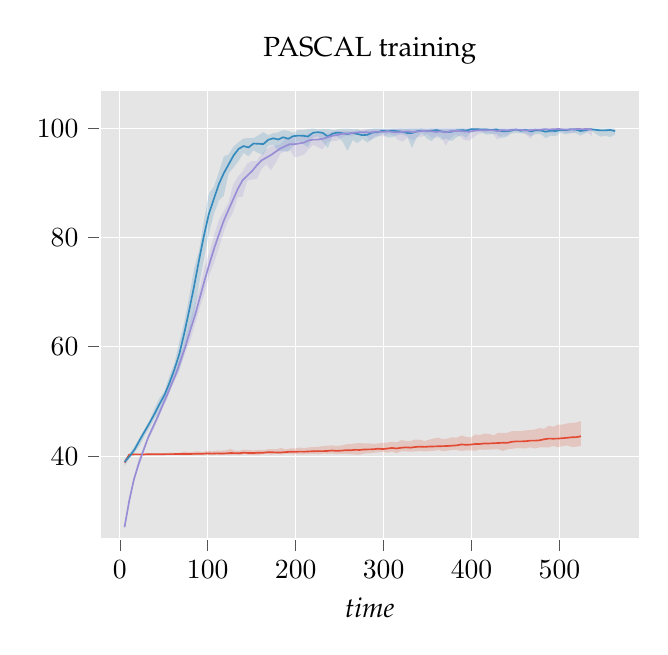
\begin{tikzpicture}

\definecolor{color0}{rgb}{0.886274509803922,0.290196078431373,0.2}
\definecolor{color1}{rgb}{0.203921568627451,0.541176470588235,0.741176470588235}
\definecolor{color2}{rgb}{0.596078431372549,0.556862745098039,0.835294117647059}

\begin{axis}[
axis background/.style={fill=white!89.8039215686275!black},
axis line style={white},
legend cell align={left},
legend style={fill opacity=0.8, draw opacity=1, text opacity=1, at={(0.97,0.03)}, anchor=south east, draw=white!80!black, fill=white!89.8039215686275!black},
log basis y={10},
tick align=outside,
tick pos=left,
title={PASCAL training},
x grid style={white},
xlabel={\textit{time}},
xmajorgrids,
xmin=-22.51834367, xmax=591.13580227,
xtick style={color=white!33.3333333333333!black},
y grid style={white},
%ylabel={accuracy},
ymajorgrids,
ymin=24.8298675401421, ymax=106.842256333744,
%ymode=log,
ytick style={color=white!33.3333333333333!black}
]
\path [fill=color0, fill opacity=0.2, very thin]
(axis cs:5.5412714,39.293156)
--(axis cs:5.5412714,38.586311)
--(axis cs:10.7587541,40.17857)
--(axis cs:15.9915457,40.193451)
--(axis cs:21.2187566,40.252975)
--(axis cs:26.4410524,40.171131)
--(axis cs:31.6724585,40.230656)
--(axis cs:36.9043758,40.186012)
--(axis cs:42.1297598,40.297619)
--(axis cs:47.3619894,40.163689)
--(axis cs:52.5935095,40.282738)
--(axis cs:57.8237142,40.200893)
--(axis cs:63.0533604,40.260418)
--(axis cs:68.291179,40.238094)
--(axis cs:73.5179721,40.163689)
--(axis cs:78.7525588,40.275299)
--(axis cs:83.9799304,40.126488)
--(axis cs:89.215081,40.238094)
--(axis cs:94.4451784,40.15625)
--(axis cs:99.6775961,40.282738)
--(axis cs:104.9103474,40.15625)
--(axis cs:110.1394607,40.230656)
--(axis cs:115.3774642,40.230656)
--(axis cs:120.6052861,40.260418)
--(axis cs:125.8343152,40.171131)
--(axis cs:131.0635599,40.245537)
--(axis cs:136.2918284,40.15625)
--(axis cs:141.5192514,40.342262)
--(axis cs:146.7505524,40.223213)
--(axis cs:151.9851635,40.223213)
--(axis cs:157.2191479,40.186012)
--(axis cs:162.4496729,40.349701)
--(axis cs:167.6752508,40.364582)
--(axis cs:172.8967094,40.245537)
--(axis cs:178.1304329,40.401787)
--(axis cs:183.3605266,40.29018)
--(axis cs:188.5837005,40.401787)
--(axis cs:193.8113178,40.372025)
--(axis cs:199.0505785,40.305061)
--(axis cs:204.3063988,40.305061)
--(axis cs:209.5681268,40.342262)
--(axis cs:214.8297355,40.357143)
--(axis cs:220.092094,40.409225)
--(axis cs:225.349245,40.319939)
--(axis cs:230.6148822,40.46875)
--(axis cs:235.8738523,40.424107)
--(axis cs:241.1424429,40.46875)
--(axis cs:246.4042916,40.379463)
--(axis cs:251.6712789,40.416668)
--(axis cs:256.9328377,40.394344)
--(axis cs:262.1820684,40.372025)
--(axis cs:267.4517359,40.29018)
--(axis cs:272.7213048,40.252975)
--(axis cs:277.9820838,40.46875)
--(axis cs:283.2400423,40.49107)
--(axis cs:288.5100395,40.610119)
--(axis cs:293.7673124,40.684525)
--(axis cs:299.0259531,40.751488)
--(axis cs:304.284308,40.632439)
--(axis cs:309.5432349,40.818451)
--(axis cs:314.8007166,40.520832)
--(axis cs:320.0586574,40.877975)
--(axis cs:325.3165302,40.855656)
--(axis cs:330.580995,40.811012)
--(axis cs:335.8395826,40.863094)
--(axis cs:341.0979941,40.907738)
--(axis cs:346.3684609,40.840775)
--(axis cs:351.630644,40.922619)
--(axis cs:356.8947862,40.944939)
--(axis cs:362.1537108,41.123512)
--(axis cs:367.4194415,40.900299)
--(axis cs:372.6863859,41.004463)
--(axis cs:377.9505458,41.145832)
--(axis cs:383.2050948,41.11607)
--(axis cs:388.4636199,40.9375)
--(axis cs:393.7022373,41.063988)
--(axis cs:398.9336173,41.063988)
--(axis cs:404.1656053,40.974701)
--(axis cs:409.3984695,41.212799)
--(axis cs:414.63383,41.160713)
--(axis cs:419.8499713,41.175594)
--(axis cs:425.0774808,41.25)
--(axis cs:430.2975157,41.257439)
--(axis cs:435.5302851,40.944939)
--(axis cs:440.7538548,41.242561)
--(axis cs:445.9886109,41.331844)
--(axis cs:451.222124,41.465775)
--(axis cs:456.4467394,41.436012)
--(axis cs:461.6752246,41.413689)
--(axis cs:466.9033261,41.599701)
--(axis cs:472.1321035,41.391369)
--(axis cs:477.3642358,41.592262)
--(axis cs:482.5978625,41.622025)
--(axis cs:487.8168653,41.607143)
--(axis cs:493.0557272,41.85268)
--(axis cs:498.2867704,41.622025)
--(axis cs:503.5192218,41.822918)
--(axis cs:508.7446351,41.956844)
--(axis cs:513.9739758,41.666668)
--(axis cs:519.1984161,41.726189)
--(axis cs:524.4339406,41.875)
--(axis cs:524.4339406,46.391369)
--(axis cs:524.4339406,46.391369)
--(axis cs:519.1984161,46.160713)
--(axis cs:513.9739758,46.049107)
--(axis cs:508.7446351,45.989582)
--(axis cs:503.5192218,45.75893)
--(axis cs:498.2867704,45.773811)
--(axis cs:493.0557272,45.386906)
--(axis cs:487.8168653,45.558037)
--(axis cs:482.5978625,45.007439)
--(axis cs:477.3642358,45.119049)
--(axis cs:472.1321035,44.873512)
--(axis cs:466.9033261,44.784225)
--(axis cs:461.6752246,44.724701)
--(axis cs:456.4467394,44.568451)
--(axis cs:451.222124,44.583332)
--(axis cs:445.9886109,44.590775)
--(axis cs:440.7538548,44.263393)
--(axis cs:435.5302851,44.248512)
--(axis cs:430.2975157,44.278275)
--(axis cs:425.0774808,43.779762)
--(axis cs:419.8499713,44.069939)
--(axis cs:414.63383,44.114582)
--(axis cs:409.3984695,43.854168)
--(axis cs:404.1656053,43.943451)
--(axis cs:398.9336173,43.400299)
--(axis cs:393.7022373,43.526787)
--(axis cs:388.4636199,43.779762)
--(axis cs:383.2050948,43.363094)
--(axis cs:377.9505458,43.452381)
--(axis cs:372.6863859,43.206844)
--(axis cs:367.4194415,43.10268)
--(axis cs:362.1537108,43.385418)
--(axis cs:356.8947862,43.236607)
--(axis cs:351.630644,42.99107)
--(axis cs:346.3684609,42.760418)
--(axis cs:341.0979941,43.035713)
--(axis cs:335.8395826,43.035713)
--(axis cs:330.580995,42.752975)
--(axis cs:325.3165302,42.797619)
--(axis cs:320.0586574,42.924107)
--(axis cs:314.8007166,42.52232)
--(axis cs:309.5432349,42.648811)
--(axis cs:304.284308,42.485119)
--(axis cs:299.0259531,42.410713)
--(axis cs:293.7673124,42.313988)
--(axis cs:288.5100395,42.232143)
--(axis cs:283.2400423,42.34375)
--(axis cs:277.9820838,42.306549)
--(axis cs:272.7213048,42.395832)
--(axis cs:267.4517359,42.32143)
--(axis cs:262.1820684,42.20982)
--(axis cs:256.9328377,42.157738)
--(axis cs:251.6712789,41.927082)
--(axis cs:246.4042916,41.837799)
--(axis cs:241.1424429,41.956844)
--(axis cs:235.8738523,41.904762)
--(axis cs:230.6148822,41.815475)
--(axis cs:225.349245,41.69643)
--(axis cs:220.092094,41.644344)
--(axis cs:214.8297355,41.599701)
--(axis cs:209.5681268,41.443451)
--(axis cs:204.3063988,41.577381)
--(axis cs:199.0505785,41.391369)
--(axis cs:193.8113178,41.398811)
--(axis cs:188.5837005,41.22768)
--(axis cs:183.3605266,41.480656)
--(axis cs:178.1304329,41.257439)
--(axis cs:172.8967094,41.309525)
--(axis cs:167.6752508,41.242561)
--(axis cs:162.4496729,41.07143)
--(axis cs:157.2191479,41.145832)
--(axis cs:151.9851635,41.034225)
--(axis cs:146.7505524,41.145832)
--(axis cs:141.5192514,41.183037)
--(axis cs:136.2918284,41.011906)
--(axis cs:131.0635599,41.019344)
--(axis cs:125.8343152,41.309525)
--(axis cs:120.6052861,41.056549)
--(axis cs:115.3774642,41.019344)
--(axis cs:110.1394607,41.004463)
--(axis cs:104.9103474,40.885418)
--(axis cs:99.6775961,40.989582)
--(axis cs:94.4451784,40.744049)
--(axis cs:89.215081,40.870537)
--(axis cs:83.9799304,40.840775)
--(axis cs:78.7525588,40.699406)
--(axis cs:73.5179721,40.863094)
--(axis cs:68.291179,40.60268)
--(axis cs:63.0533604,40.595238)
--(axis cs:57.8237142,40.64732)
--(axis cs:52.5935095,40.520832)
--(axis cs:47.3619894,40.476189)
--(axis cs:42.1297598,40.431549)
--(axis cs:36.9043758,40.498512)
--(axis cs:31.6724585,40.572918)
--(axis cs:26.4410524,40.416668)
--(axis cs:21.2187566,40.379463)
--(axis cs:15.9915457,40.520832)
--(axis cs:10.7587541,40.349701)
--(axis cs:5.5412714,39.293156)
--cycle;

\path [fill=color1, fill opacity=0.2, very thin]
(axis cs:5.6260672,39.561012)
--(axis cs:5.6260672,38.139881)
--(axis cs:11.2535209,39.657738)
--(axis cs:16.8821791,40.669643)
--(axis cs:22.5129408,41.919643)
--(axis cs:28.1409546,43.705357)
--(axis cs:33.7698938,45.141369)
--(axis cs:39.3974973,46.85268)
--(axis cs:45.0289549,47.938988)
--(axis cs:50.6595453,50.163689)
--(axis cs:56.2911642,51.875)
--(axis cs:61.9214925,53.943451)
--(axis cs:67.5537216,55.684525)
--(axis cs:73.1848777,58.809525)
--(axis cs:78.8136691,62.901787)
--(axis cs:84.4452633,66.011902)
--(axis cs:90.0816605,71.421127)
--(axis cs:95.7124145,76.041664)
--(axis cs:101.3411513,80.751488)
--(axis cs:106.968866,84.278275)
--(axis cs:112.6002733,86.741074)
--(axis cs:118.2328614,87.626488)
--(axis cs:123.86435,91.770836)
--(axis cs:129.4952305,92.790176)
--(axis cs:135.1272681,94.01786)
--(axis cs:140.7567669,95.46875)
--(axis cs:146.3903903,94.821426)
--(axis cs:152.0240724,95.9375)
--(axis cs:157.6550483,95.386902)
--(axis cs:163.2870228,95.171127)
--(axis cs:168.9189764,96.778275)
--(axis cs:174.550778,96.979164)
--(axis cs:180.1811305,95.803574)
--(axis cs:185.8129355,95.78125)
--(axis cs:191.445592,95.654762)
--(axis cs:197.0751451,96.733627)
--(axis cs:202.7054722,97.678574)
--(axis cs:208.3360316,97.098213)
--(axis cs:213.9661486,96.495537)
--(axis cs:219.6007554,98.311012)
--(axis cs:225.2331292,98.497025)
--(axis cs:230.866702,97.447914)
--(axis cs:236.5017746,96.331848)
--(axis cs:242.1326346,98.645836)
--(axis cs:247.7625551,98.415176)
--(axis cs:253.3940067,97.507439)
--(axis cs:259.0275111,95.848213)
--(axis cs:264.6597033,97.760414)
--(axis cs:270.2932876,97.254463)
--(axis cs:275.9243725,98.01339)
--(axis cs:281.5556128,97.358627)
--(axis cs:287.1860658,98.005951)
--(axis cs:292.8193899,98.385414)
--(axis cs:298.4521344,99.025299)
--(axis cs:304.0827333,98.273811)
--(axis cs:309.7165831,98.340775)
--(axis cs:315.3511348,98.697914)
--(axis cs:320.982853,98.854164)
--(axis cs:326.6176425,98.541664)
--(axis cs:332.2509906,96.376488)
--(axis cs:337.8810316,98.318451)
--(axis cs:343.5135627,99.122025)
--(axis cs:349.146443,98.087799)
--(axis cs:354.7785734,97.596725)
--(axis cs:360.4141405,98.697914)
--(axis cs:366.0440321,97.85714)
--(axis cs:371.675223,98.043152)
--(axis cs:377.3079713,97.641373)
--(axis cs:382.9392785,98.318451)
--(axis cs:388.5707666,98.720238)
--(axis cs:394.2052504,98.244049)
--(axis cs:399.8375876,99.508926)
--(axis cs:405.4716968,99.382439)
--(axis cs:411.1050251,99.360123)
--(axis cs:416.7358429,98.787201)
--(axis cs:422.3713528,98.891373)
--(axis cs:428.0033261,98.943451)
--(axis cs:433.6350751,98.199402)
--(axis cs:439.2657704,98.363098)
--(axis cs:444.8985152,98.988098)
--(axis cs:450.5346249,99.129463)
--(axis cs:456.1709546,99.047623)
--(axis cs:461.8075688,99.010414)
--(axis cs:467.4402806,98.571426)
--(axis cs:473.0721336,98.891373)
--(axis cs:478.706084,98.883926)
--(axis cs:484.341686,98.162201)
--(axis cs:489.9755157,98.623512)
--(axis cs:495.6105514,98.504463)
--(axis cs:501.2437495,99.159225)
--(axis cs:506.8807368,98.824402)
--(axis cs:512.5182115,99.203873)
--(axis cs:518.1546725,99.122025)
--(axis cs:523.7902731,98.59375)
--(axis cs:529.4256998,99.0625)
--(axis cs:535.0610824,99.64286)
--(axis cs:540.6960484,99.032738)
--(axis cs:546.330671,98.422623)
--(axis cs:551.9697797,98.616074)
--(axis cs:557.6055358,98.363098)
--(axis cs:563.242432,98.831848)
--(axis cs:563.242432,99.940475)
--(axis cs:563.242432,99.940475)
--(axis cs:557.6055358,99.970238)
--(axis cs:551.9697797,99.940475)
--(axis cs:546.330671,99.940475)
--(axis cs:540.6960484,99.925598)
--(axis cs:535.0610824,99.977676)
--(axis cs:529.4256998,99.933037)
--(axis cs:523.7902731,99.910713)
--(axis cs:518.1546725,99.977676)
--(axis cs:512.5182115,99.962799)
--(axis cs:506.8807368,99.985123)
--(axis cs:501.2437495,99.970238)
--(axis cs:495.6105514,99.970238)
--(axis cs:489.9755157,99.962799)
--(axis cs:484.341686,99.970238)
--(axis cs:478.706084,99.880951)
--(axis cs:473.0721336,99.910713)
--(axis cs:467.4402806,99.910713)
--(axis cs:461.8075688,99.925598)
--(axis cs:456.1709546,99.940475)
--(axis cs:450.5346249,99.977676)
--(axis cs:444.8985152,99.95536)
--(axis cs:439.2657704,99.970238)
--(axis cs:433.6350751,99.970238)
--(axis cs:428.0033261,99.970238)
--(axis cs:422.3713528,99.95536)
--(axis cs:416.7358429,99.985123)
--(axis cs:411.1050251,99.985123)
--(axis cs:405.4716968,99.985123)
--(axis cs:399.8375876,99.977676)
--(axis cs:394.2052504,99.970238)
--(axis cs:388.5707666,99.977676)
--(axis cs:382.9392785,99.977676)
--(axis cs:377.3079713,99.947914)
--(axis cs:371.675223,99.95536)
--(axis cs:366.0440321,99.925598)
--(axis cs:360.4141405,99.977676)
--(axis cs:354.7785734,99.962799)
--(axis cs:349.146443,99.903275)
--(axis cs:343.5135627,99.985123)
--(axis cs:337.8810316,99.962799)
--(axis cs:332.2509906,99.933037)
--(axis cs:326.6176425,99.933037)
--(axis cs:320.982853,99.947914)
--(axis cs:315.3511348,99.910713)
--(axis cs:309.7165831,99.903275)
--(axis cs:304.0827333,99.880951)
--(axis cs:298.4521344,99.925598)
--(axis cs:292.8193899,99.962799)
--(axis cs:287.1860658,99.918152)
--(axis cs:281.5556128,99.747025)
--(axis cs:275.9243725,99.427086)
--(axis cs:270.2932876,99.858627)
--(axis cs:264.6597033,99.828873)
--(axis cs:259.0275111,99.918152)
--(axis cs:253.3940067,99.925598)
--(axis cs:247.7625551,99.761902)
--(axis cs:242.1326346,99.650299)
--(axis cs:236.5017746,99.880951)
--(axis cs:230.866702,99.873512)
--(axis cs:225.2331292,99.761902)
--(axis cs:219.6007554,99.933037)
--(axis cs:213.9661486,99.813988)
--(axis cs:208.3360316,99.672623)
--(axis cs:202.7054722,99.650299)
--(axis cs:197.0751451,99.114586)
--(axis cs:191.445592,99.501488)
--(axis cs:185.8129355,99.635414)
--(axis cs:180.1811305,99.211311)
--(axis cs:174.550778,99.084824)
--(axis cs:168.9189764,98.683037)
--(axis cs:163.2870228,99.278275)
--(axis cs:157.6550483,98.690475)
--(axis cs:152.0240724,98.16964)
--(axis cs:146.3903903,98.162201)
--(axis cs:140.7567669,98.125)
--(axis cs:135.1272681,97.418152)
--(axis cs:129.4952305,96.696426)
--(axis cs:123.86435,95.186012)
--(axis cs:118.2328614,94.813988)
--(axis cs:112.6002733,91.912201)
--(axis cs:106.968866,89.278275)
--(axis cs:101.3411513,88.058037)
--(axis cs:95.7124145,83.08036)
--(axis cs:90.0816605,77.589287)
--(axis cs:84.4452633,74.308037)
--(axis cs:78.8136691,69.099701)
--(axis cs:73.1848777,64.464287)
--(axis cs:67.5537216,60.818451)
--(axis cs:61.9214925,56.904762)
--(axis cs:56.2911642,54.590775)
--(axis cs:50.6595453,51.808037)
--(axis cs:45.0289549,50.580357)
--(axis cs:39.3974973,48.645832)
--(axis cs:33.7698938,46.5625)
--(axis cs:28.1409546,44.970238)
--(axis cs:22.5129408,43.430061)
--(axis cs:16.8821791,41.822918)
--(axis cs:11.2535209,40.513393)
--(axis cs:5.6260672,39.561012)
--cycle;

\path [fill=color2, fill opacity=0.2, very thin]
(axis cs:5.3750266,27.455357)
--(axis cs:5.3750266,26.532738)
--(axis cs:10.7446771,31.153274)
--(axis cs:16.1140605,35.267857)
--(axis cs:21.4814285,37.998512)
--(axis cs:26.8506366,40.505952)
--(axis cs:32.2191005,42.97619)
--(axis cs:37.5907383,44.52381)
--(axis cs:42.9568892,46.525298)
--(axis cs:48.3279217,48.779762)
--(axis cs:53.6960726,50.342262)
--(axis cs:59.0655616,52.678571)
--(axis cs:64.4351531,54.479167)
--(axis cs:69.8046928,56.599702)
--(axis cs:75.1736773,59.22619)
--(axis cs:80.5431057,61.324405)
--(axis cs:85.914368,64.241071)
--(axis cs:91.2816405,67.425595)
--(axis cs:96.6499017,69.895833)
--(axis cs:102.01895,73.27381)
--(axis cs:107.3914175,75.401786)
--(axis cs:112.7613681,78.169643)
--(axis cs:118.1308767,80.967262)
--(axis cs:123.5008418,83.110119)
--(axis cs:128.871909,84.613095)
--(axis cs:134.2417003,87.425595)
--(axis cs:139.6114576,87.418155)
--(axis cs:144.9815286,90.394345)
--(axis cs:150.3534418,90.602679)
--(axis cs:155.7232912,90.714286)
--(axis cs:161.0921416,92.49256)
--(axis cs:166.4616942,93.385417)
--(axis cs:171.8328728,92.299107)
--(axis cs:177.2010011,93.60119)
--(axis cs:182.570106,95.31994)
--(axis cs:187.9389139,95.77381)
--(axis cs:193.3095832,95.997024)
--(axis cs:198.6790512,94.657738)
--(axis cs:204.0480883,94.873512)
--(axis cs:209.4172138,95.14881)
--(axis cs:214.7856931,96.183036)
--(axis cs:220.1553017,96.949405)
--(axis cs:225.5241256,96.465774)
--(axis cs:230.8949159,96.116071)
--(axis cs:236.2650776,97.544643)
--(axis cs:241.6301539,97.559524)
--(axis cs:246.9982468,97.700893)
--(axis cs:252.3648026,98.251488)
--(axis cs:257.7343132,98.59375)
--(axis cs:263.1035713,98.489583)
--(axis cs:268.4729623,98.824405)
--(axis cs:273.8437403,98.861607)
--(axis cs:279.2109044,98.883929)
--(axis cs:284.5796196,97.678571)
--(axis cs:289.9484996,98.519345)
--(axis cs:295.3162435,98.549107)
--(axis cs:300.6853035,98.474702)
--(axis cs:306.0530288,98.854167)
--(axis cs:311.4243238,98.59375)
--(axis cs:316.7940289,97.797619)
--(axis cs:322.1636215,97.544643)
--(axis cs:327.5318684,98.348214)
--(axis cs:332.9005789,97.715774)
--(axis cs:338.2699809,98.296131)
--(axis cs:343.640863,98.407738)
--(axis cs:349.0089287,98.91369)
--(axis cs:354.3781891,98.28869)
--(axis cs:359.7465708,98.184524)
--(axis cs:365.1134055,98.534226)
--(axis cs:370.4793936,96.778274)
--(axis cs:375.8500088,98.125)
--(axis cs:381.2190867,98.809524)
--(axis cs:386.5882787,98.526786)
--(axis cs:391.9570295,97.790179)
--(axis cs:397.3292076,97.730655)
--(axis cs:402.6982975,98.348214)
--(axis cs:408.0645675,98.936012)
--(axis cs:413.4340398,99.077381)
--(axis cs:418.8024688,99.06994)
--(axis cs:424.1712483,98.943452)
--(axis cs:429.5398063,97.872024)
--(axis cs:434.9091743,98.735119)
--(axis cs:440.2767364,98.645833)
--(axis cs:445.6456363,99.345238)
--(axis cs:451.0159235,99.53869)
--(axis cs:456.3836459,99.270833)
--(axis cs:461.7496335,98.831845)
--(axis cs:467.1185583,98.072917)
--(axis cs:472.4850222,99.315476)
--(axis cs:477.8604424,99.181548)
--(axis cs:483.2285335,99.613095)
--(axis cs:488.5950382,99.077381)
--(axis cs:493.9652527,99.040179)
--(axis cs:499.3330222,99.441964)
--(axis cs:504.7005091,99.278274)
--(axis cs:510.0699591,98.995536)
--(axis cs:515.4392375,99.032738)
--(axis cs:520.8047162,99.494048)
--(axis cs:526.1734665,99.144345)
--(axis cs:531.5429649,99.241071)
--(axis cs:536.9092059,98.556548)
--(axis cs:536.9092059,99.977679)
--(axis cs:536.9092059,99.977679)
--(axis cs:531.5429649,99.977679)
--(axis cs:526.1734665,99.977679)
--(axis cs:520.8047162,99.970238)
--(axis cs:515.4392375,99.970238)
--(axis cs:510.0699591,99.962798)
--(axis cs:504.7005091,99.970238)
--(axis cs:499.3330222,99.970238)
--(axis cs:493.9652527,99.947917)
--(axis cs:488.5950382,99.903274)
--(axis cs:483.2285335,99.933036)
--(axis cs:477.8604424,99.970238)
--(axis cs:472.4850222,99.933036)
--(axis cs:467.1185583,99.977679)
--(axis cs:461.7496335,99.962798)
--(axis cs:456.3836459,99.895833)
--(axis cs:451.0159235,99.955357)
--(axis cs:445.6456363,99.933036)
--(axis cs:440.2767364,99.925595)
--(axis cs:434.9091743,99.947917)
--(axis cs:429.5398063,99.933036)
--(axis cs:424.1712483,99.962798)
--(axis cs:418.8024688,99.962798)
--(axis cs:413.4340398,99.947917)
--(axis cs:408.0645675,99.947917)
--(axis cs:402.6982975,99.933036)
--(axis cs:397.3292076,99.940476)
--(axis cs:391.9570295,99.962798)
--(axis cs:386.5882787,99.918155)
--(axis cs:381.2190867,99.955357)
--(axis cs:375.8500088,99.962798)
--(axis cs:370.4793936,99.962798)
--(axis cs:365.1134055,99.940476)
--(axis cs:359.7465708,99.933036)
--(axis cs:354.3781891,99.977679)
--(axis cs:349.0089287,99.962798)
--(axis cs:343.640863,99.947917)
--(axis cs:338.2699809,99.925595)
--(axis cs:332.9005789,99.955357)
--(axis cs:327.5318684,99.918155)
--(axis cs:322.1636215,99.910714)
--(axis cs:316.7940289,99.962798)
--(axis cs:311.4243238,99.947917)
--(axis cs:306.0530288,99.858631)
--(axis cs:300.6853035,99.84375)
--(axis cs:295.3162435,99.754464)
--(axis cs:289.9484996,99.813988)
--(axis cs:284.5796196,99.784226)
--(axis cs:279.2109044,99.85119)
--(axis cs:273.8437403,99.672619)
--(axis cs:268.4729623,99.479167)
--(axis cs:263.1035713,99.375)
--(axis cs:257.7343132,99.479167)
--(axis cs:252.3648026,99.494048)
--(axis cs:246.9982468,99.575893)
--(axis cs:241.6301539,99.300595)
--(axis cs:236.2650776,99.017857)
--(axis cs:230.8949159,98.973214)
--(axis cs:225.5241256,98.973214)
--(axis cs:220.1553017,98.712798)
--(axis cs:214.7856931,99.047619)
--(axis cs:209.4172138,98.58631)
--(axis cs:204.0480883,98.720238)
--(axis cs:198.6790512,98.370536)
--(axis cs:193.3095832,98.392857)
--(axis cs:187.9389139,97.983631)
--(axis cs:182.570106,97.046131)
--(axis cs:177.2010011,96.837798)
--(axis cs:171.8328728,96.71131)
--(axis cs:166.4616942,96.08631)
--(axis cs:161.0921416,95.252976)
--(axis cs:155.7232912,94.017857)
--(axis cs:150.3534418,93.936012)
--(axis cs:144.9815286,93.534226)
--(axis cs:139.6114576,92.053571)
--(axis cs:134.2417003,91.09375)
--(axis cs:128.871909,89.665179)
--(axis cs:123.5008418,86.309524)
--(axis cs:118.1308767,84.784226)
--(axis cs:112.7613681,83.221726)
--(axis cs:107.3914175,80.453869)
--(axis cs:102.01895,77.373512)
--(axis cs:96.6499017,74.739583)
--(axis cs:91.2816405,70.974702)
--(axis cs:85.914368,68.258929)
--(axis cs:80.5431057,64.955357)
--(axis cs:75.1736773,61.860119)
--(axis cs:69.8046928,59.040179)
--(axis cs:64.4351531,56.183036)
--(axis cs:59.0655616,53.816964)
--(axis cs:53.6960726,52.373512)
--(axis cs:48.3279217,49.880952)
--(axis cs:42.9568892,47.752976)
--(axis cs:37.5907383,45.736607)
--(axis cs:32.2191005,43.779762)
--(axis cs:26.8506366,41.525298)
--(axis cs:21.4814285,39.434524)
--(axis cs:16.1140605,36.227679)
--(axis cs:10.7446771,32.730655)
--(axis cs:5.3750266,27.455357)
--cycle;

\addplot [semithick, color0]
table {%
5.5412712097168 38.8288688659668
10.7587537765503 40.2686004638672
15.9915456771851 40.3132476806641
21.2187557220459 40.3184471130371
26.4410514831543 40.2983665466309
31.6724586486816 40.3422584533691
36.9043769836426 40.3258972167969
42.1297607421875 40.3489608764648
47.361988067627 40.3266372680664
52.5935096740723 40.363094329834
57.8237152099609 40.3586311340332
68.2911758422852 40.3943481445312
78.752555847168 40.386157989502
89.2150802612305 40.4300575256348
94.4451751708984 40.4315452575684
99.6775970458984 40.4977645874023
104.910346984863 40.4516372680664
110.139457702637 40.5
115.377464294434 40.4761924743652
120.605285644531 40.4962768554688
125.834312438965 40.5625
136.29182434082 40.53125
141.519256591797 40.6339340209961
146.750549316406 40.5595283508301
151.985168457031 40.5647277832031
157.219146728516 40.6108627319336
162.449676513672 40.6086349487305
167.675247192383 40.6994018554688
172.896713256836 40.7083282470703
178.130432128906 40.6666717529297
183.36051940918 40.6726226806641
193.811325073242 40.7953910827637
199.050582885742 40.7819976806641
204.306396484375 40.8251533508301
209.568130493164 40.8110122680664
214.829742431641 40.8571472167969
225.349243164062 40.921875
230.614883422852 40.9062538146973
235.87385559082 40.9456825256348
241.142440795898 41.0238037109375
246.404296875 40.9598236083984
251.671279907227 41.0000038146973
256.932830810547 41.0766372680664
262.182067871094 41.0617561340332
267.451721191406 41.1540145874023
272.721313476562 41.1250038146973
277.982086181641 41.222469329834
283.240051269531 41.2254447937012
288.510040283203 41.2566986083984
293.767303466797 41.3563957214355
299.025939941406 41.2797622680664
309.543243408203 41.492561340332
314.800720214844 41.3980674743652
320.058654785156 41.5305023193359
325.316528320312 41.6071472167969
330.580993652344 41.5431594848633
335.839569091797 41.6621971130371
341.097991943359 41.7328834533691
346.368469238281 41.6919631958008
351.630645751953 41.7447967529297
372.686370849609 41.8496971130371
383.205108642578 41.9717292785645
388.463623046875 42.1309509277344
393.702239990234 42.0699462890625
398.933624267578 42.105655670166
404.165618896484 42.210563659668
409.398468017578 42.2202415466309
414.633819580078 42.3162155151367
419.849975585938 42.3139839172363
435.5302734375 42.4404716491699
440.753845214844 42.426342010498
445.988616943359 42.6287231445312
451.222137451172 42.6934547424316
456.446746826172 42.6964340209961
461.675231933594 42.722469329834
466.9033203125 42.8318481445312
472.132110595703 42.8281211853027
477.364227294922 42.8921089172363
482.597869873047 43.086311340332
487.816864013672 43.199405670166
493.055725097656 43.1860084533691
498.286773681641 43.2053604125977
508.74462890625 43.3519287109375
513.973999023438 43.4479217529297
519.198425292969 43.4739532470703
524.433959960938 43.6331825256348
};
%\addlegendentry{cudnn}
\addplot [semithick, color1]
table {%
5.62606716156006 38.9724731445312
11.2535209655762 39.9866027832031
16.8821792602539 41.2306518554688
22.5129413604736 42.8928604125977
28.1409549713135 44.488094329834
33.7698936462402 46.0409202575684
39.3974990844727 47.694938659668
45.0289535522461 49.4843826293945
50.6595458984375 51.1227684020996
56.2911643981934 53.3095283508301
61.9214935302734 55.7663650512695
67.5537185668945 58.5967330932617
73.1848754882812 62.3935966491699
78.8136672973633 66.5639877319336
84.4452667236328 71.0662231445312
90.081657409668 75.8296127319336
95.7124176025391 80.3496932983398
101.341148376465 84.3489608764648
112.600273132324 89.7313919067383
118.232864379883 91.7492446899414
129.495223999023 95.0252990722656
135.12727355957 96.2016296386719
140.756759643555 96.7135238647461
146.390396118164 96.4709777832031
152.024078369141 97.1755905151367
163.287017822266 97.0818481445312
168.918975830078 97.8720169067383
174.55078125 98.1331939697266
180.181137084961 97.9203796386719
185.812942504883 98.3303527832031
191.445587158203 98.0446395874023
197.075149536133 98.5178680419922
202.705474853516 98.6272354125977
208.336029052734 98.6078796386719
213.966156005859 98.4546127319336
219.60075378418 99.1406326293945
225.233123779297 99.2566833496094
230.86669921875 99.1279830932617
236.501770019531 98.4479064941406
242.132629394531 98.9947967529297
247.762557983398 99.1815490722656
259.027496337891 98.9233627319336
264.659698486328 99.1235198974609
275.924377441406 98.7068557739258
281.555603027344 98.7730712890625
287.186065673828 99.1979064941406
292.819396972656 99.2314071655273
298.4521484375 99.5275192260742
304.082733154297 99.3995513916016
309.716583251953 99.5297546386719
320.982849121094 99.3422698974609
326.617645263672 99.1153335571289
332.2509765625 99.1056442260742
337.881042480469 99.421875
343.513549804688 99.5163726806641
349.146453857422 99.4040298461914
360.414154052734 99.6346664428711
366.044036865234 99.3868942260742
371.675231933594 99.2723236083984
377.307983398438 99.3437423706055
382.939270019531 99.5476226806641
388.570770263672 99.6317138671875
394.205261230469 99.5483627319336
399.837585449219 99.805793762207
416.73583984375 99.749267578125
422.371337890625 99.6421051025391
428.003326416016 99.7596740722656
433.635070800781 99.4627914428711
439.265777587891 99.4025268554688
444.898529052734 99.5364456176758
450.534637451172 99.7284317016602
456.170959472656 99.5245361328125
461.807556152344 99.6755828857422
467.440277099609 99.4025268554688
473.072143554688 99.601936340332
478.706085205078 99.5788650512695
484.341674804688 99.3385391235352
489.975524902344 99.5260391235352
495.610565185547 99.4627914428711
501.243743896484 99.6696472167969
506.880737304688 99.602668762207
512.518188476562 99.7775268554688
518.154663085938 99.7470245361328
523.790283203125 99.4664993286133
535.061096191406 99.8005905151367
546.330688476562 99.5877990722656
551.969787597656 99.5848236083984
557.605529785156 99.6555099487305
563.242431640625 99.4568405151367
};
%\addlegendentry{libtorch}
\addplot [semithick, color2]
table {%
5.37502670288086 27.0059547424316
10.7446775436401 31.8556575775146
16.1140613555908 35.7730674743652
21.4814281463623 38.59375
26.8506374359131 41.0245590209961
32.2191009521484 43.3965759277344
37.5907402038574 45.2857055664062
42.9568901062012 47.1302032470703
53.6960716247559 51.1488189697266
64.4351501464844 55.3132400512695
69.8046951293945 57.8132514953613
75.1736755371094 60.2879524230957
80.5431060791016 63.2447967529297
85.9143676757812 65.9754409790039
91.2816390991211 69.1354141235352
96.64990234375 72.2760391235352
102.018951416016 75.2388381958008
107.391418457031 78.0520858764648
112.761367797852 80.5803680419922
118.130874633789 83.0200805664062
123.500839233398 85.0133895874023
134.24169921875 88.8876571655273
139.611450195312 90.4613037109375
150.353439331055 92.1368865966797
155.723297119141 93.1741104125977
161.092147827148 94.0855712890625
171.832870483398 95.0743942260742
182.570098876953 96.2700958251953
193.309585571289 97.0654907226562
198.679046630859 97.0520858764648
209.417221069336 97.3511810302734
214.785690307617 97.7566986083984
220.155303955078 97.8906326293945
225.524124145508 97.9017868041992
230.894912719727 98.0520935058594
241.630157470703 98.5974578857422
246.998245239258 98.7202453613281
252.364807128906 98.9412307739258
263.103576660156 99.0833435058594
268.472961425781 99.1986694335938
273.84375 99.258918762207
284.579620361328 99.2128067016602
289.948486328125 99.319938659668
300.685302734375 99.313232421875
306.053039550781 99.4062347412109
311.42431640625 99.2299118041992
316.794036865234 99.2440490722656
327.531860351562 99.4025268554688
332.900573730469 99.2514801025391
343.640869140625 99.4746932983398
354.378204345703 99.4196319580078
359.74658203125 99.2775344848633
365.113403320312 99.4099731445312
370.479400634766 99.212043762207
375.850006103516 99.4598159790039
386.588287353516 99.4888381958008
391.95703125 99.3802108764648
397.329193115234 99.3325958251953
402.698303222656 99.4970321655273
408.064575195312 99.6108703613281
424.171234130859 99.6272277832031
429.539794921875 99.4293212890625
434.9091796875 99.6488037109375
440.276733398438 99.5595092773438
445.645629882812 99.6934509277344
456.383636474609 99.6778335571289
461.749633789062 99.5617523193359
467.118560791016 99.6138305664062
472.485015869141 99.7299118041992
477.860443115234 99.7090835571289
483.228546142578 99.7991104125977
488.595031738281 99.7581939697266
499.3330078125 99.8474731445312
504.700500488281 99.7254486083984
510.069946289062 99.727668762207
520.8046875 99.8422622680664
526.173461914062 99.8080444335938
531.54296875 99.8489532470703
536.9091796875 99.7090835571289
};
%\addlegendentry{pytorch}
\end{axis}

\end{tikzpicture}

        \end{adjustbox}
      \end{subfigure}
      \begin{subfigure}{0.24\textwidth}
        \centering
        \begin{adjustbox}{width=\textwidth}
          % This file was created by tikzplotlib v0.9.5.
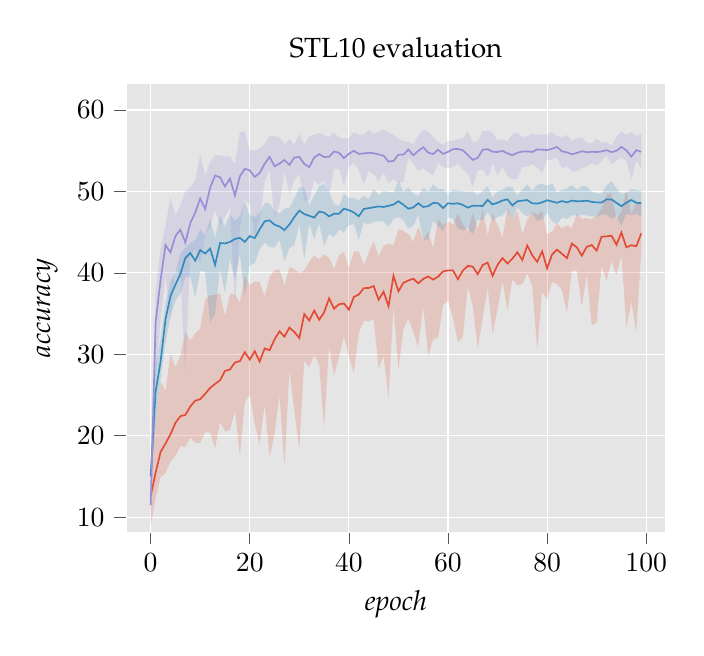
\begin{tikzpicture}

\definecolor{color0}{rgb}{0.886274509803922,0.290196078431373,0.2}
\definecolor{color1}{rgb}{0.203921568627451,0.541176470588235,0.741176470588235}
\definecolor{color2}{rgb}{0.596078431372549,0.556862745098039,0.835294117647059}

\begin{axis}[
axis background/.style={fill=white!89.8039215686275!black},
axis line style={white},
legend cell align={left},
legend style={fill opacity=0.8, draw opacity=1, text opacity=1, at={(0.97,0.03)}, anchor=south east, draw=white!80!black, fill=white!89.8039215686275!black},
log basis y={10},
tick align=outside,
tick pos=left,
title={STL10 evaluation},
x grid style={white},
xlabel={\textit{epoch}},
xmajorgrids,
xmin=-4.95, xmax=103.95,
xtick style={color=white!33.3333333333333!black},
y grid style={white},
ylabel={\textit{accuracy}},
ymajorgrids,
ymin=8.15863803616345, ymax=63.2058278627682,
%ymode=log,
ytick style={color=white!33.3333333333333!black}
]
\path [fill=color0, fill opacity=0.2, very thin]
(axis cs:0,17.6282)
--(axis cs:0,8.95433)
--(axis cs:1,12.3798)
--(axis cs:2,14.9038)
--(axis cs:3,15.4247)
--(axis cs:4,16.867)
--(axis cs:5,17.508)
--(axis cs:6,18.73)
--(axis cs:7,18.5897)
--(axis cs:8,19.7516)
--(axis cs:9,19.1707)
--(axis cs:10,19.1306)
--(axis cs:11,20.4527)
--(axis cs:12,20.3926)
--(axis cs:13,18.4896)
--(axis cs:14,21.6747)
--(axis cs:15,20.5529)
--(axis cs:16,20.6731)
--(axis cs:17,23.0769)
--(axis cs:18,17.528)
--(axis cs:19,24.0585)
--(axis cs:20,25.02)
--(axis cs:21,21.4944)
--(axis cs:22,18.9704)
--(axis cs:23,23.7981)
--(axis cs:24,17.4279)
--(axis cs:25,20.1723)
--(axis cs:26,24.9599)
--(axis cs:27,16.246)
--(axis cs:28,28.145)
--(axis cs:29,23.0369)
--(axis cs:30,18.4095)
--(axis cs:31,29.1867)
--(axis cs:32,28.4054)
--(axis cs:33,29.9079)
--(axis cs:34,28.7861)
--(axis cs:35,20.9535)
--(axis cs:36,30.9896)
--(axis cs:37,27.4038)
--(axis cs:38,29.6875)
--(axis cs:39,32.2316)
--(axis cs:40,29.7676)
--(axis cs:41,27.6843)
--(axis cs:42,32.6322)
--(axis cs:43,34.1346)
--(axis cs:44,33.9944)
--(axis cs:45,34.375)
--(axis cs:46,28.2652)
--(axis cs:47,29.8678)
--(axis cs:48,24.5994)
--(axis cs:49,35.9375)
--(axis cs:50,28.0849)
--(axis cs:51,33.133)
--(axis cs:52,34.4151)
--(axis cs:53,32.7324)
--(axis cs:54,30.9095)
--(axis cs:55,35.8574)
--(axis cs:56,29.7877)
--(axis cs:57,31.8109)
--(axis cs:58,32.0312)
--(axis cs:59,36.0577)
--(axis cs:60,36.5585)
--(axis cs:61,34.4551)
--(axis cs:62,31.5104)
--(axis cs:63,32.1114)
--(axis cs:64,38.3213)
--(axis cs:65,35.9175)
--(axis cs:66,30.7492)
--(axis cs:67,34.355)
--(axis cs:68,38.2612)
--(axis cs:69,32.472)
--(axis cs:70,35.4968)
--(axis cs:71,38.9623)
--(axis cs:72,35.4167)
--(axis cs:73,39.2027)
--(axis cs:74,38.4615)
--(axis cs:75,38.6218)
--(axis cs:76,39.9639)
--(axis cs:77,38.4014)
--(axis cs:78,30.4688)
--(axis cs:79,37.6202)
--(axis cs:80,36.7588)
--(axis cs:81,38.8622)
--(axis cs:82,38.6418)
--(axis cs:83,37.8806)
--(axis cs:84,35.0761)
--(axis cs:85,40.2644)
--(axis cs:86,40.2845)
--(axis cs:87,35.8574)
--(axis cs:88,39.8037)
--(axis cs:89,33.5537)
--(axis cs:90,33.9143)
--(axis cs:91,40.9054)
--(axis cs:92,39.0224)
--(axis cs:93,41.4062)
--(axis cs:94,39.6835)
--(axis cs:95,42.0673)
--(axis cs:96,33.2933)
--(axis cs:97,36.4383)
--(axis cs:98,32.6522)
--(axis cs:99,42.7083)
--(axis cs:99,48.6979)
--(axis cs:99,48.6979)
--(axis cs:98,48.6779)
--(axis cs:97,47.1955)
--(axis cs:96,50.1402)
--(axis cs:95,47.516)
--(axis cs:94,46.6146)
--(axis cs:93,49.7796)
--(axis cs:92,49.6194)
--(axis cs:91,47.9167)
--(axis cs:90,46.9952)
--(axis cs:89,46.5946)
--(axis cs:88,46.7348)
--(axis cs:87,46.6346)
--(axis cs:86,47.2756)
--(axis cs:85,45.5128)
--(axis cs:84,45.8333)
--(axis cs:83,45.4928)
--(axis cs:82,46.0537)
--(axis cs:81,45.0521)
--(axis cs:80,44.7516)
--(axis cs:79,47.6162)
--(axis cs:78,47.1154)
--(axis cs:77,47.516)
--(axis cs:76,46.5345)
--(axis cs:75,44.7316)
--(axis cs:74,47.6562)
--(axis cs:73,46.4744)
--(axis cs:72,48.0168)
--(axis cs:71,44.3109)
--(axis cs:70,45.9135)
--(axis cs:69,47.2957)
--(axis cs:68,44.6514)
--(axis cs:67,47.7163)
--(axis cs:66,45.3926)
--(axis cs:65,47.3758)
--(axis cs:64,45.0321)
--(axis cs:63,46.0337)
--(axis cs:62,47.3157)
--(axis cs:61,45.9135)
--(axis cs:60,46.3742)
--(axis cs:59,45.8534)
--(axis cs:58,46.5545)
--(axis cs:57,43.0489)
--(axis cs:56,45.0321)
--(axis cs:55,44.0505)
--(axis cs:54,45.653)
--(axis cs:53,43.7901)
--(axis cs:52,44.7917)
--(axis cs:51,45.1522)
--(axis cs:50,45.3926)
--(axis cs:49,43.3694)
--(axis cs:48,43.5897)
--(axis cs:47,43.3293)
--(axis cs:46,42.0272)
--(axis cs:45,43.9103)
--(axis cs:44,42.4479)
--(axis cs:43,40.9655)
--(axis cs:42,42.6482)
--(axis cs:41,42.6282)
--(axis cs:40,40.605)
--(axis cs:39,42.5681)
--(axis cs:38,42.1675)
--(axis cs:37,40.4647)
--(axis cs:36,41.847)
--(axis cs:35,42.2877)
--(axis cs:34,41.6266)
--(axis cs:33,42.1675)
--(axis cs:32,41.3662)
--(axis cs:31,40.3245)
--(axis cs:30,39.984)
--(axis cs:29,40.4247)
--(axis cs:28,40.7252)
--(axis cs:27,38.4215)
--(axis cs:26,40.4447)
--(axis cs:25,40.3045)
--(axis cs:24,39.5232)
--(axis cs:23,37.0793)
--(axis cs:22,38.8822)
--(axis cs:21,38.9623)
--(axis cs:20,38.5216)
--(axis cs:19,39.5833)
--(axis cs:18,36.3782)
--(axis cs:17,37.3397)
--(axis cs:16,37.4399)
--(axis cs:15,34.6755)
--(axis cs:14,37.52)
--(axis cs:13,37.2596)
--(axis cs:12,37.2796)
--(axis cs:11,36.7588)
--(axis cs:10,33.1931)
--(axis cs:9,32.5921)
--(axis cs:8,31.6707)
--(axis cs:7,32.8325)
--(axis cs:6,29.7877)
--(axis cs:5,28.4455)
--(axis cs:4,30.0881)
--(axis cs:3,25.5409)
--(axis cs:2,26.6426)
--(axis cs:1,21.7949)
--(axis cs:0,17.6282)
--cycle;

\path [fill=color1, fill opacity=0.2, very thin]
(axis cs:0,16.4062)
--(axis cs:0,12.9836)
--(axis cs:1,21.5526)
--(axis cs:2,26.9717)
--(axis cs:3,31.3988)
--(axis cs:4,34.7098)
--(axis cs:5,36.5203)
--(axis cs:6,37.4628)
--(axis cs:7,39.4717)
--(axis cs:8,39.5709)
--(axis cs:9,36.9048)
--(axis cs:10,40.2902)
--(axis cs:11,40.1166)
--(axis cs:12,33.8914)
--(axis cs:13,35.0074)
--(axis cs:14,40.5134)
--(axis cs:15,37.5248)
--(axis cs:16,41.7287)
--(axis cs:17,39.1245)
--(axis cs:18,42.3239)
--(axis cs:19,36.9916)
--(axis cs:20,40.9474)
--(axis cs:21,41.1706)
--(axis cs:22,42.8943)
--(axis cs:23,43.7004)
--(axis cs:24,43.1796)
--(axis cs:25,43.1176)
--(axis cs:26,44.0352)
--(axis cs:27,41.3938)
--(axis cs:28,43.0432)
--(axis cs:29,43.3656)
--(axis cs:30,45.9573)
--(axis cs:31,41.6915)
--(axis cs:32,46.0565)
--(axis cs:33,44.1096)
--(axis cs:34,46.0441)
--(axis cs:35,43.2664)
--(axis cs:36,44.7793)
--(axis cs:37,44.3824)
--(axis cs:38,45.3125)
--(axis cs:39,44.9529)
--(axis cs:40,45.8705)
--(axis cs:41,45.9697)
--(axis cs:42,44.0724)
--(axis cs:43,46.2054)
--(axis cs:44,45.9573)
--(axis cs:45,46.255)
--(axis cs:46,46.379)
--(axis cs:47,46.2798)
--(axis cs:48,45.6721)
--(axis cs:49,46.6146)
--(axis cs:50,46.8626)
--(axis cs:51,46.4286)
--(axis cs:52,45.4489)
--(axis cs:53,45.7713)
--(axis cs:54,47.061)
--(axis cs:55,44.1096)
--(axis cs:56,44.06)
--(axis cs:57,46.4286)
--(axis cs:58,45.6845)
--(axis cs:59,45.0893)
--(axis cs:60,46.7386)
--(axis cs:61,46.7138)
--(axis cs:62,45.4613)
--(axis cs:63,45.2009)
--(axis cs:64,45.5109)
--(axis cs:65,44.6677)
--(axis cs:66,46.503)
--(axis cs:67,46.4906)
--(axis cs:68,47.4082)
--(axis cs:69,46.4782)
--(axis cs:70,46.8626)
--(axis cs:71,47.0362)
--(axis cs:72,47.7679)
--(axis cs:73,46.5154)
--(axis cs:74,48.0655)
--(axis cs:75,47.3338)
--(axis cs:76,46.9246)
--(axis cs:77,47.3462)
--(axis cs:78,46.3914)
--(axis cs:79,46.565)
--(axis cs:80,47.371)
--(axis cs:81,46.3666)
--(axis cs:82,45.9449)
--(axis cs:83,46.813)
--(axis cs:84,46.5898)
--(axis cs:85,47.0982)
--(axis cs:86,47.0114)
--(axis cs:87,47.0858)
--(axis cs:88,47.061)
--(axis cs:89,46.937)
--(axis cs:90,46.8874)
--(axis cs:91,47.185)
--(axis cs:92,47.1478)
--(axis cs:93,46.627)
--(axis cs:94,46.9742)
--(axis cs:95,45.7713)
--(axis cs:96,47.247)
--(axis cs:97,47.0734)
--(axis cs:98,47.2346)
--(axis cs:99,46.937)
--(axis cs:99,50.062)
--(axis cs:99,50.062)
--(axis cs:98,50.2108)
--(axis cs:97,50.2976)
--(axis cs:96,49.8264)
--(axis cs:95,49.7148)
--(axis cs:94,50.3968)
--(axis cs:93,51.2401)
--(axis cs:92,50.7564)
--(axis cs:91,49.7272)
--(axis cs:90,49.7644)
--(axis cs:89,49.9628)
--(axis cs:88,50.6324)
--(axis cs:87,50.6572)
--(axis cs:86,50.2232)
--(axis cs:85,50.8061)
--(axis cs:84,50.4216)
--(axis cs:83,50.186)
--(axis cs:82,49.8636)
--(axis cs:81,50.9797)
--(axis cs:80,50.7068)
--(axis cs:79,50.9673)
--(axis cs:78,50.8061)
--(axis cs:77,50.0496)
--(axis cs:76,50.8433)
--(axis cs:75,50.2356)
--(axis cs:74,49.4916)
--(axis cs:73,50.5456)
--(axis cs:72,50.6076)
--(axis cs:71,50.2232)
--(axis cs:70,50.0248)
--(axis cs:69,49.2932)
--(axis cs:68,50.6324)
--(axis cs:67,50.0124)
--(axis cs:66,49.5536)
--(axis cs:65,50.0248)
--(axis cs:64,49.9752)
--(axis cs:63,50.0372)
--(axis cs:62,50.124)
--(axis cs:61,50.1984)
--(axis cs:60,49.7396)
--(axis cs:59,50.248)
--(axis cs:58,50.3224)
--(axis cs:57,50.8557)
--(axis cs:56,49.9628)
--(axis cs:55,50.4712)
--(axis cs:54,49.4544)
--(axis cs:53,49.7272)
--(axis cs:52,50.4836)
--(axis cs:51,49.9876)
--(axis cs:50,51.2773)
--(axis cs:49,49.8264)
--(axis cs:48,49.9752)
--(axis cs:47,50.0372)
--(axis cs:46,49.5288)
--(axis cs:45,50.3348)
--(axis cs:44,49.0699)
--(axis cs:43,49.4544)
--(axis cs:42,48.8839)
--(axis cs:41,49.2312)
--(axis cs:40,49.1815)
--(axis cs:39,49.7396)
--(axis cs:38,48.2143)
--(axis cs:37,48.4747)
--(axis cs:36,49.814)
--(axis cs:35,50.9301)
--(axis cs:34,50.6696)
--(axis cs:33,49.4792)
--(axis cs:32,48.2763)
--(axis cs:31,50.4712)
--(axis cs:30,50.5084)
--(axis cs:29,49.1443)
--(axis cs:28,47.9663)
--(axis cs:27,47.9167)
--(axis cs:26,47.309)
--(axis cs:25,47.5694)
--(axis cs:24,48.5367)
--(axis cs:23,48.5739)
--(axis cs:22,47.4082)
--(axis cs:21,46.8378)
--(axis cs:20,47.1106)
--(axis cs:19,48.7599)
--(axis cs:18,46.9866)
--(axis cs:17,46.3914)
--(axis cs:16,47.2098)
--(axis cs:15,45.7341)
--(axis cs:14,47.0238)
--(axis cs:13,44.2832)
--(axis cs:12,46.627)
--(axis cs:11,44.6305)
--(axis cs:10,45.3249)
--(axis cs:9,44.0848)
--(axis cs:8,43.7004)
--(axis cs:7,43.0804)
--(axis cs:6,42.4107)
--(axis cs:5,40.0546)
--(axis cs:4,38.9509)
--(axis cs:3,36.2847)
--(axis cs:2,31.8576)
--(axis cs:1,28.7946)
--(axis cs:0,16.4062)
--cycle;

\path [fill=color2, fill opacity=0.2, very thin]
(axis cs:0,17.559524)
--(axis cs:0,9.920635)
--(axis cs:1,27.157738)
--(axis cs:2,34.126984)
--(axis cs:3,39.657738)
--(axis cs:4,34.126984)
--(axis cs:5,40.562996)
--(axis cs:6,39.459325)
--(axis cs:7,27.641369)
--(axis cs:8,42.199901)
--(axis cs:9,42.906746)
--(axis cs:10,41.09623)
--(axis cs:11,44.53125)
--(axis cs:12,45.62252)
--(axis cs:13,47.730655)
--(axis cs:14,45.696925)
--(axis cs:15,46.875)
--(axis cs:16,48.040675)
--(axis cs:17,35.900298)
--(axis cs:18,45.337302)
--(axis cs:19,48.970734)
--(axis cs:20,48.375496)
--(axis cs:21,44.419643)
--(axis cs:22,46.540179)
--(axis cs:23,51.202877)
--(axis cs:24,52.616567)
--(axis cs:25,46.701389)
--(axis cs:26,48.338294)
--(axis cs:27,52.405754)
--(axis cs:28,49.739583)
--(axis cs:29,51.364087)
--(axis cs:30,52.18254)
--(axis cs:31,48.797123)
--(axis cs:32,49.007937)
--(axis cs:33,51.326885)
--(axis cs:34,50.830853)
--(axis cs:35,51.339286)
--(axis cs:36,49.553571)
--(axis cs:37,52.752976)
--(axis cs:38,52.790179)
--(axis cs:39,50.669643)
--(axis cs:40,52.97619)
--(axis cs:41,53.509425)
--(axis cs:42,52.542163)
--(axis cs:43,50.818452)
--(axis cs:44,52.554563)
--(axis cs:45,52.070933)
--(axis cs:46,51.25248)
--(axis cs:47,52.34375)
--(axis cs:48,51.016865)
--(axis cs:49,51.550099)
--(axis cs:50,51.066468)
--(axis cs:51,51.153274)
--(axis cs:52,54.154266)
--(axis cs:53,53.397817)
--(axis cs:54,52.480159)
--(axis cs:55,52.839782)
--(axis cs:56,52.281746)
--(axis cs:57,51.984127)
--(axis cs:58,53.509425)
--(axis cs:59,53.013393)
--(axis cs:60,52.864583)
--(axis cs:61,53.025794)
--(axis cs:62,53.410218)
--(axis cs:63,52.666171)
--(axis cs:64,52.157738)
--(axis cs:65,50.508433)
--(axis cs:66,52.641369)
--(axis cs:67,52.628968)
--(axis cs:68,51.72371)
--(axis cs:69,53.410218)
--(axis cs:70,51.984127)
--(axis cs:71,53.062996)
--(axis cs:72,51.87252)
--(axis cs:73,51.500496)
--(axis cs:74,51.5625)
--(axis cs:75,52.96379)
--(axis cs:76,53.062996)
--(axis cs:77,53.311012)
--(axis cs:78,52.926587)
--(axis cs:79,52.294147)
--(axis cs:80,53.856647)
--(axis cs:81,53.955853)
--(axis cs:82,54.154266)
--(axis cs:83,52.790179)
--(axis cs:84,53.075397)
--(axis cs:85,52.517361)
--(axis cs:86,52.442956)
--(axis cs:87,52.876984)
--(axis cs:88,53.050595)
--(axis cs:89,53.459821)
--(axis cs:90,53.174603)
--(axis cs:91,53.732639)
--(axis cs:92,54.389881)
--(axis cs:93,53.323413)
--(axis cs:94,53.769841)
--(axis cs:95,54.141865)
--(axis cs:96,53.769841)
--(axis cs:97,51.438492)
--(axis cs:98,53.769841)
--(axis cs:99,52.839782)
--(axis cs:99,57.056052)
--(axis cs:99,57.056052)
--(axis cs:98,56.783234)
--(axis cs:97,57.328869)
--(axis cs:96,56.919643)
--(axis cs:95,57.390873)
--(axis cs:94,56.646825)
--(axis cs:93,55.61756)
--(axis cs:92,56.076389)
--(axis cs:91,56.026786)
--(axis cs:90,56.460813)
--(axis cs:89,55.902778)
--(axis cs:88,55.989583)
--(axis cs:87,56.597222)
--(axis cs:86,56.535218)
--(axis cs:85,56.163194)
--(axis cs:84,56.932044)
--(axis cs:83,56.671627)
--(axis cs:82,56.795635)
--(axis cs:81,57.328869)
--(axis cs:80,56.969246)
--(axis cs:79,57.018849)
--(axis cs:78,56.932044)
--(axis cs:77,57.093254)
--(axis cs:76,56.820437)
--(axis cs:75,56.646825)
--(axis cs:74,57.254464)
--(axis cs:73,56.994048)
--(axis cs:72,56.125992)
--(axis cs:71,56.436012)
--(axis cs:70,56.25)
--(axis cs:69,57.217262)
--(axis cs:68,57.477679)
--(axis cs:67,57.390873)
--(axis cs:66,56.187996)
--(axis cs:65,56.001984)
--(axis cs:64,57.428075)
--(axis cs:63,56.56002)
--(axis cs:62,56.39881)
--(axis cs:61,56.212798)
--(axis cs:60,56.225198)
--(axis cs:59,55.741567)
--(axis cs:58,56.076389)
--(axis cs:57,56.696429)
--(axis cs:56,57.366071)
--(axis cs:55,57.589286)
--(axis cs:54,56.87004)
--(axis cs:53,55.803571)
--(axis cs:52,56.08879)
--(axis cs:51,56.175595)
--(axis cs:50,56.41121)
--(axis cs:49,56.932044)
--(axis cs:48,57.217262)
--(axis cs:47,57.576885)
--(axis cs:46,57.291667)
--(axis cs:45,57.105655)
--(axis cs:44,57.576885)
--(axis cs:43,56.994048)
--(axis cs:42,56.981647)
--(axis cs:41,57.254464)
--(axis cs:40,56.584821)
--(axis cs:39,56.473214)
--(axis cs:38,56.597222)
--(axis cs:37,57.291667)
--(axis cs:36,56.659226)
--(axis cs:35,56.944444)
--(axis cs:34,57.18006)
--(axis cs:33,56.969246)
--(axis cs:32,56.733631)
--(axis cs:31,55.753968)
--(axis cs:30,57.105655)
--(axis cs:29,55.716766)
--(axis cs:28,56.460813)
--(axis cs:27,55.766369)
--(axis cs:26,56.646825)
--(axis cs:25,56.783234)
--(axis cs:24,56.808036)
--(axis cs:23,55.803571)
--(axis cs:22,55.332341)
--(axis cs:21,54.985119)
--(axis cs:20,55.109127)
--(axis cs:19,57.390873)
--(axis cs:18,57.291667)
--(axis cs:17,53.28621)
--(axis cs:16,54.340278)
--(axis cs:15,54.265873)
--(axis cs:14,54.451885)
--(axis cs:13,54.427083)
--(axis cs:12,53.583829)
--(axis cs:11,51.946925)
--(axis cs:10,54.551091)
--(axis cs:9,51.364087)
--(axis cs:8,50.520833)
--(axis cs:7,49.987599)
--(axis cs:6,48.301091)
--(axis cs:5,47.085813)
--(axis cs:4,49.305556)
--(axis cs:3,45.758929)
--(axis cs:2,42.993552)
--(axis cs:1,37.475198)
--(axis cs:0,17.559524)
--cycle;

\addplot [semithick, color0]
table {%
0 12.5921440124512
1 15.4647483825684
2 18.0088024139404
3 19.0444927215576
4 20.1862983703613
5 21.5905494689941
6 22.4138793945312
7 22.5560913085938
8 23.6037673950195
9 24.3089065551758
10 24.4911861419678
11 25.1522426605225
12 25.8713893890381
13 26.3681926727295
14 26.8128986358643
15 27.9627380371094
16 28.1390209197998
17 28.9903736114502
18 29.1686515808105
19 30.2704257965088
20 29.3529644012451
21 30.3805866241455
22 29.1145935058594
23 30.7211513519287
24 30.504810333252
25 31.8329238891602
26 32.8225288391113
27 32.1674652099609
28 33.285270690918
29 32.7383804321289
30 31.9991912841797
31 34.9319000244141
32 34.1586494445801
33 35.3806266784668
34 34.244800567627
35 35.1462326049805
36 36.8769950866699
37 35.6129608154297
38 36.1418151855469
39 36.2439956665039
40 35.4727554321289
41 37.0372543334961
42 37.3477401733398
43 38.1250038146973
44 38.147029876709
45 38.3894348144531
46 36.6967124938965
47 37.6943130493164
48 35.9114646911621
49 39.6414184570312
50 37.736385345459
51 38.7740173339844
52 39.0685157775879
53 39.2828598022461
54 38.7199554443359
55 39.2548027038574
56 39.563304901123
57 39.1686553955078
58 39.5412750244141
59 40.178295135498
60 40.3084869384766
61 40.3125038146973
62 39.2187347412109
63 40.2824630737305
64 40.861385345459
65 40.7632179260254
66 39.8317489624023
67 40.9695625305176
68 41.2499961853027
69 39.6334228515625
70 40.9875946044922
71 41.8169136047363
72 41.1478462219238
73 41.7568092346191
74 42.5320434570312
75 41.58251953125
76 43.3653907775879
77 42.1574172973633
78 41.3541717529297
79 42.6342010498047
80 40.5629043579102
81 42.255615234375
82 42.8505554199219
83 42.3497505187988
84 41.8088760375977
85 43.5997543334961
86 43.1390228271484
87 42.1133766174316
88 43.2031173706055
89 43.4194755554199
90 42.7303771972656
91 44.4451179504395
92 44.4811706542969
93 44.5693016052246
94 43.4555320739746
95 44.9579391479492
96 43.1410331726074
97 43.3954429626465
98 43.271240234375
99 44.8457450866699
};
%\addlegendentry{cudnn}
\addplot [semithick, color1]
table {%
0 15.0198402404785
1 25.394344329834
2 29.0972175598145
3 34.3043174743652
4 37.168888092041
5 38.5528182983398
6 39.8635902404785
7 41.8278732299805
8 42.429313659668
9 41.4980278015137
10 42.7864761352539
11 42.3797149658203
12 42.9724655151367
13 40.9945259094238
14 43.6718711853027
15 43.6098556518555
16 43.7983551025391
17 44.1530303955078
18 44.2956275939941
19 43.8070487976074
20 44.5151252746582
21 44.2708320617676
22 45.3620834350586
23 46.324405670166
24 46.4508972167969
25 45.9089813232422
26 45.6981506347656
27 45.2480201721191
28 45.9548759460449
29 46.8675575256348
30 47.6450843811035
31 47.2259140014648
33 46.7894439697266
34 47.5260391235352
35 47.3995628356934
36 46.933292388916
37 47.2594223022461
38 47.2631454467773
39 47.8807029724121
40 47.6984062194824
41 47.4206314086914
42 46.9506492614746
43 47.8398094177246
46 48.1572456359863
47 48.0915145874023
49 48.386661529541
50 48.7946548461914
51 48.3655853271484
52 47.8794555664062
53 48.0356979370117
54 48.5478744506836
55 48.090274810791
56 48.1894836425781
57 48.5962448120117
58 48.5453948974609
59 47.9575843811035
60 48.5416793823242
61 48.477180480957
62 48.5429039001465
63 48.3395347595215
64 48.0071868896484
65 48.2539710998535
67 48.2118034362793
68 48.9670143127441
69 48.4065055847168
70 48.6086235046387
71 48.8901252746582
72 49.0277786254883
73 48.2713279724121
74 48.7909317016602
76 48.944694519043
77 48.5379486083984
78 48.5069427490234
79 48.6495513916016
80 48.9186248779297
82 48.6073989868164
83 48.8182067871094
84 48.6507911682129
85 48.8752593994141
86 48.7921524047852
87 48.8082656860352
88 48.8616027832031
89 48.7177543640137
90 48.6557464599609
91 48.6371612548828
92 49.0277633666992
93 49.0104217529297
95 48.1907424926758
96 48.6197929382324
97 48.9508857727051
98 48.612361907959
99 48.5652160644531
};
%\addlegendentry{libtorch}
\addplot [semithick, color2]
table {%
0 11.4918165206909
1 33.9298133850098
2 39.0959777832031
3 43.4102172851562
4 42.5123977661133
5 44.5250473022461
6 45.2988624572754
7 43.7214813232422
8 46.1185569763184
9 47.4045219421387
10 49.1331825256348
11 47.8286209106445
12 50.4464302062988
13 51.9568481445312
14 51.7299156188965
15 50.613842010498
16 51.5922660827637
17 49.4903297424316
18 51.8477210998535
19 52.7864532470703
20 52.5830841064453
21 51.7881965637207
22 52.2681121826172
23 53.3916091918945
24 54.2447967529297
25 53.0952377319336
26 53.4226150512695
27 53.8554077148438
28 53.2490119934082
29 54.1679153442383
30 54.2261848449707
31 53.3792152404785
32 52.9898262023926
33 54.1505508422852
34 54.5808486938477
35 54.2249488830566
36 54.2571830749512
37 54.9045143127441
38 54.7519836425781
39 54.0910263061523
40 54.6180610656738
41 54.9888381958008
42 54.6068916320801
44 54.7371063232422
45 54.6961822509766
47 54.3836860656738
48 53.6706275939941
49 53.7425537109375
50 54.5138893127441
51 54.5151329040527
52 55.1475677490234
53 54.4345207214355
54 54.9801597595215
55 55.4303169250488
56 54.7643852233887
57 54.5820922851562
58 55.1314506530762
59 54.604419708252
60 54.8561592102051
61 55.1909675598145
62 55.2170181274414
63 55.0545654296875
65 53.8727645874023
66 54.1306953430176
67 55.1178169250488
68 55.187255859375
69 54.8722724914551
70 54.8375511169434
71 54.9876022338867
72 54.6664161682129
73 54.4580917358398
74 54.7445449829102
75 54.9045143127441
76 54.9144325256348
77 54.8449859619141
78 55.1587257385254
80 55.0806121826172
81 55.2368621826172
82 55.4575881958008
83 54.9256019592285
84 54.7966232299805
85 54.5684432983398
86 54.7172622680664
87 54.9330368041992
88 54.8139839172363
89 54.863597869873
90 54.8363151550293
91 54.9131965637207
92 55.0681991577148
93 54.8288650512695
94 54.9888381958008
95 55.4600677490234
96 55.0458793640137
97 54.2757873535156
98 55.0620002746582
99 54.8598785400391
};
%\addlegendentry{pytorch}
\end{axis}

\end{tikzpicture}

        \end{adjustbox}
      \end{subfigure}
      \begin{subfigure}{0.24\textwidth}
        \centering
        \begin{adjustbox}{width=\textwidth}
          % This file was created by tikzplotlib v0.9.5.
\begin{tikzpicture}





\begin{axis}[
axis background/.style={fill=white!89.8039215686275!black},
axis line style={white},
legend cell align={left},
legend style={fill opacity=0.8, draw opacity=1, text opacity=1, draw=white!80!black, fill=white!89.8039215686275!black},
log basis y={10},
tick align=outside,
tick pos=left,
title={PASCAL evaluation},
x grid style={white},
xlabel={epoch},
xmajorgrids,
xmin=-4.95, xmax=103.95,
xtick style={color=white!33.3333333333333!black},
y grid style={white},
%ylabel={accuracy},
ymajorgrids,
ymin=12.524687588205, ymax=96.7215659804425,
%ymode=log,
ytick style={color=white!33.3333333333333!black}
]
\path [fill=cudnn, fill opacity=0.2, very thin]
(axis cs:0,40.3329)
--(axis cs:0,39.632)
--(axis cs:1,39.5444)
--(axis cs:2,39.6904)
--(axis cs:3,39.5444)
--(axis cs:4,39.6904)
--(axis cs:5,39.5736)
--(axis cs:6,39.7488)
--(axis cs:7,39.5152)
--(axis cs:8,39.5736)
--(axis cs:9,39.6612)
--(axis cs:10,39.3692)
--(axis cs:11,39.6028)
--(axis cs:12,39.3107)
--(axis cs:13,39.5444)
--(axis cs:14,39.5152)
--(axis cs:15,39.6028)
--(axis cs:16,39.4276)
--(axis cs:17,39.6612)
--(axis cs:18,39.632)
--(axis cs:19,39.6612)
--(axis cs:20,39.7488)
--(axis cs:21,39.778)
--(axis cs:22,39.632)
--(axis cs:23,39.632)
--(axis cs:24,39.5152)
--(axis cs:25,39.7196)
--(axis cs:26,39.7196)
--(axis cs:27,39.6904)
--(axis cs:28,39.5444)
--(axis cs:29,39.7196)
--(axis cs:30,39.7196)
--(axis cs:31,39.6028)
--(axis cs:32,39.486)
--(axis cs:33,39.7196)
--(axis cs:34,39.486)
--(axis cs:35,39.632)
--(axis cs:36,39.6612)
--(axis cs:37,39.4568)
--(axis cs:38,39.6612)
--(axis cs:39,39.8072)
--(axis cs:40,39.8364)
--(axis cs:41,39.778)
--(axis cs:42,39.6612)
--(axis cs:43,39.632)
--(axis cs:44,39.6612)
--(axis cs:45,39.9241)
--(axis cs:46,39.7488)
--(axis cs:47,39.7196)
--(axis cs:48,39.5152)
--(axis cs:49,39.7196)
--(axis cs:50,39.6028)
--(axis cs:51,39.6612)
--(axis cs:52,40.0117)
--(axis cs:53,40.2745)
--(axis cs:54,40.0117)
--(axis cs:55,39.9241)
--(axis cs:56,39.9825)
--(axis cs:57,39.9825)
--(axis cs:58,39.9825)
--(axis cs:59,39.9241)
--(axis cs:60,39.9241)
--(axis cs:61,40.1285)
--(axis cs:62,40.3037)
--(axis cs:63,39.8657)
--(axis cs:64,40.0117)
--(axis cs:65,40.0117)
--(axis cs:66,40.0993)
--(axis cs:67,40.0117)
--(axis cs:68,40.0993)
--(axis cs:69,40.1577)
--(axis cs:70,40.2745)
--(axis cs:71,40.2161)
--(axis cs:72,39.9533)
--(axis cs:73,40.1869)
--(axis cs:74,40.0117)
--(axis cs:75,39.9241)
--(axis cs:76,40.1869)
--(axis cs:77,40.0701)
--(axis cs:78,40.3037)
--(axis cs:79,40.3329)
--(axis cs:80,40.1577)
--(axis cs:81,40.1869)
--(axis cs:82,40.3329)
--(axis cs:83,40.0117)
--(axis cs:84,40.2161)
--(axis cs:85,40.2745)
--(axis cs:86,40.1285)
--(axis cs:87,40.2161)
--(axis cs:88,40.4206)
--(axis cs:89,40.2453)
--(axis cs:90,39.9825)
--(axis cs:91,40.2161)
--(axis cs:92,40.2453)
--(axis cs:93,40.3329)
--(axis cs:94,40.5666)
--(axis cs:95,40.1869)
--(axis cs:96,40.3037)
--(axis cs:97,40.2161)
--(axis cs:98,40.3037)
--(axis cs:99,40.1869)
--(axis cs:99,42.1437)
--(axis cs:99,42.1437)
--(axis cs:98,42.1437)
--(axis cs:97,42.2021)
--(axis cs:96,42.0853)
--(axis cs:95,41.9685)
--(axis cs:94,42.6402)
--(axis cs:93,42.1437)
--(axis cs:92,41.9393)
--(axis cs:91,42.1729)
--(axis cs:90,42.3189)
--(axis cs:89,42.4942)
--(axis cs:88,42.2897)
--(axis cs:87,42.4065)
--(axis cs:86,42.2021)
--(axis cs:85,42.7862)
--(axis cs:84,43.2243)
--(axis cs:83,42.7278)
--(axis cs:82,42.4942)
--(axis cs:81,42.8738)
--(axis cs:80,42.8446)
--(axis cs:79,42.3189)
--(axis cs:78,42.465)
--(axis cs:77,42.6986)
--(axis cs:76,42.6402)
--(axis cs:75,43.0199)
--(axis cs:74,43.1951)
--(axis cs:73,42.611)
--(axis cs:72,42.6402)
--(axis cs:71,42.2313)
--(axis cs:70,42.4065)
--(axis cs:69,42.6986)
--(axis cs:68,42.465)
--(axis cs:67,42.7862)
--(axis cs:66,42.5234)
--(axis cs:65,42.6402)
--(axis cs:64,42.465)
--(axis cs:63,42.1145)
--(axis cs:62,42.3189)
--(axis cs:61,42.4065)
--(axis cs:60,42.4942)
--(axis cs:59,42.3481)
--(axis cs:58,42.5234)
--(axis cs:57,42.0853)
--(axis cs:56,42.4942)
--(axis cs:55,42.1145)
--(axis cs:54,42.1729)
--(axis cs:53,41.7348)
--(axis cs:52,42.0561)
--(axis cs:51,41.9393)
--(axis cs:50,41.8224)
--(axis cs:49,41.7056)
--(axis cs:48,41.6472)
--(axis cs:47,41.472)
--(axis cs:46,41.5596)
--(axis cs:45,41.472)
--(axis cs:44,41.2967)
--(axis cs:43,41.4136)
--(axis cs:42,41.4136)
--(axis cs:41,41.3259)
--(axis cs:40,41.2967)
--(axis cs:39,41.2675)
--(axis cs:38,41.0923)
--(axis cs:37,41.3843)
--(axis cs:36,40.9171)
--(axis cs:35,41.1507)
--(axis cs:34,40.9463)
--(axis cs:33,41.0047)
--(axis cs:32,41.0339)
--(axis cs:31,40.9171)
--(axis cs:30,40.8294)
--(axis cs:29,40.771)
--(axis cs:28,40.8002)
--(axis cs:27,40.7126)
--(axis cs:26,40.6834)
--(axis cs:25,40.9171)
--(axis cs:24,40.8586)
--(axis cs:23,40.6834)
--(axis cs:22,40.5958)
--(axis cs:21,40.625)
--(axis cs:20,40.5958)
--(axis cs:19,40.5666)
--(axis cs:18,40.2745)
--(axis cs:17,40.5082)
--(axis cs:16,40.3621)
--(axis cs:15,40.5082)
--(axis cs:14,40.4498)
--(axis cs:13,40.2745)
--(axis cs:12,40.2745)
--(axis cs:11,40.2745)
--(axis cs:10,40.2453)
--(axis cs:9,40.2161)
--(axis cs:8,40.3914)
--(axis cs:7,40.0993)
--(axis cs:6,40.2745)
--(axis cs:5,40.1285)
--(axis cs:4,40.3037)
--(axis cs:3,40.2745)
--(axis cs:2,40.2745)
--(axis cs:1,40.3621)
--(axis cs:0,40.3329)
--cycle;

\path [fill=libtorch, fill opacity=0.2, very thin]
(axis cs:0,39.7569)
--(axis cs:0,35.9086)
--(axis cs:1,27.8067)
--(axis cs:2,31.4815)
--(axis cs:3,18.8368)
--(axis cs:4,19.4734)
--(axis cs:5,15.6829)
--(axis cs:6,21.0938)
--(axis cs:7,28.0093)
--(axis cs:8,13.7442)
--(axis cs:9,31.8576)
--(axis cs:10,32.5521)
--(axis cs:11,28.4144)
--(axis cs:12,26.0995)
--(axis cs:13,23.5822)
--(axis cs:14,25.0579)
--(axis cs:15,32.5521)
--(axis cs:16,28.3275)
--(axis cs:17,24.4502)
--(axis cs:18,27.2569)
--(axis cs:19,30.5556)
--(axis cs:20,25.2894)
--(axis cs:21,28.1829)
--(axis cs:22,30.787)
--(axis cs:23,32.3206)
--(axis cs:24,35.9086)
--(axis cs:25,31.8866)
--(axis cs:26,34.6933)
--(axis cs:27,33.1308)
--(axis cs:28,35.6192)
--(axis cs:29,33.8252)
--(axis cs:30,29.89)
--(axis cs:31,37.037)
--(axis cs:32,39.5255)
--(axis cs:33,37.5579)
--(axis cs:34,31.1632)
--(axis cs:35,33.8252)
--(axis cs:36,31.5394)
--(axis cs:37,33.912)
--(axis cs:38,38.9178)
--(axis cs:39,40.0463)
--(axis cs:40,31.4525)
--(axis cs:41,35.4456)
--(axis cs:42,40.7697)
--(axis cs:43,39.2072)
--(axis cs:44,38.0498)
--(axis cs:45,36.2847)
--(axis cs:46,38.831)
--(axis cs:47,38.4549)
--(axis cs:48,35.3009)
--(axis cs:49,38.3391)
--(axis cs:50,40.1331)
--(axis cs:51,40.7407)
--(axis cs:52,41.2037)
--(axis cs:53,41.3194)
--(axis cs:54,41.6377)
--(axis cs:55,41.7245)
--(axis cs:56,28.9931)
--(axis cs:57,36.7477)
--(axis cs:58,40.2199)
--(axis cs:59,42.5347)
--(axis cs:60,36.4873)
--(axis cs:61,40.6829)
--(axis cs:62,38.7442)
--(axis cs:63,40.1331)
--(axis cs:64,41.4352)
--(axis cs:65,40.5382)
--(axis cs:66,39.9884)
--(axis cs:67,40.5093)
--(axis cs:68,42.3322)
--(axis cs:69,40.5671)
--(axis cs:70,40.8275)
--(axis cs:71,42.1875)
--(axis cs:72,42.3032)
--(axis cs:73,42.1296)
--(axis cs:74,41.5799)
--(axis cs:75,41.0012)
--(axis cs:76,36.7188)
--(axis cs:77,39.9306)
--(axis cs:78,41.1748)
--(axis cs:79,42.4479)
--(axis cs:80,43.2002)
--(axis cs:81,40.0752)
--(axis cs:82,41.2905)
--(axis cs:83,41.3484)
--(axis cs:84,41.4352)
--(axis cs:85,36.4583)
--(axis cs:86,38.5127)
--(axis cs:87,42.4769)
--(axis cs:88,41.1458)
--(axis cs:89,42.5926)
--(axis cs:90,42.7373)
--(axis cs:91,40.3067)
--(axis cs:92,41.7824)
--(axis cs:93,42.3611)
--(axis cs:94,41.8981)
--(axis cs:95,41.1169)
--(axis cs:96,41.1748)
--(axis cs:97,39.9016)
--(axis cs:98,39.4676)
--(axis cs:99,39.7859)
--(axis cs:99,45.9491)
--(axis cs:99,45.9491)
--(axis cs:98,46.0069)
--(axis cs:97,46.2674)
--(axis cs:96,44.9942)
--(axis cs:95,46.0938)
--(axis cs:94,46.7882)
--(axis cs:93,46.0648)
--(axis cs:92,46.5567)
--(axis cs:91,44.9653)
--(axis cs:90,46.6146)
--(axis cs:89,46.7014)
--(axis cs:88,46.3252)
--(axis cs:87,45.4861)
--(axis cs:86,45.515)
--(axis cs:85,46.2963)
--(axis cs:84,45.6887)
--(axis cs:83,44.3287)
--(axis cs:82,45.7755)
--(axis cs:81,45.6019)
--(axis cs:80,45.081)
--(axis cs:79,46.6146)
--(axis cs:78,45.5729)
--(axis cs:77,46.7014)
--(axis cs:76,46.1227)
--(axis cs:75,46.4988)
--(axis cs:74,46.0359)
--(axis cs:73,45.8623)
--(axis cs:72,47.338)
--(axis cs:71,46.2095)
--(axis cs:70,47.4826)
--(axis cs:69,46.0938)
--(axis cs:68,45.978)
--(axis cs:67,45.1389)
--(axis cs:66,47.0197)
--(axis cs:65,46.0938)
--(axis cs:64,44.9942)
--(axis cs:63,46.3252)
--(axis cs:62,45.4861)
--(axis cs:61,45.8333)
--(axis cs:60,46.2095)
--(axis cs:59,45.2836)
--(axis cs:58,45.1678)
--(axis cs:57,44.4444)
--(axis cs:56,45.081)
--(axis cs:55,47.2801)
--(axis cs:54,46.6435)
--(axis cs:53,46.1516)
--(axis cs:52,45.3704)
--(axis cs:51,45.8333)
--(axis cs:50,44.647)
--(axis cs:49,45.11)
--(axis cs:48,44.7049)
--(axis cs:47,44.0972)
--(axis cs:46,45.9491)
--(axis cs:45,45.9201)
--(axis cs:44,44.6759)
--(axis cs:43,44.8495)
--(axis cs:42,46.2963)
--(axis cs:41,44.8206)
--(axis cs:40,45.4572)
--(axis cs:39,45.3414)
--(axis cs:38,45.544)
--(axis cs:37,45.7176)
--(axis cs:36,45.9201)
--(axis cs:35,45.7176)
--(axis cs:34,44.8785)
--(axis cs:33,44.213)
--(axis cs:32,46.0648)
--(axis cs:31,45.1968)
--(axis cs:30,43.7789)
--(axis cs:29,45.0521)
--(axis cs:28,43.4896)
--(axis cs:27,44.5891)
--(axis cs:26,44.7049)
--(axis cs:25,43.3738)
--(axis cs:24,44.2708)
--(axis cs:23,44.184)
--(axis cs:22,42.5926)
--(axis cs:21,43.7211)
--(axis cs:20,43.0556)
--(axis cs:19,44.4155)
--(axis cs:18,41.3773)
--(axis cs:17,43.5475)
--(axis cs:16,40.7118)
--(axis cs:15,40.4225)
--(axis cs:14,40.3067)
--(axis cs:13,39.4965)
--(axis cs:12,44.9653)
--(axis cs:11,43.8368)
--(axis cs:10,45.11)
--(axis cs:9,41.4352)
--(axis cs:8,44.0683)
--(axis cs:7,44.8785)
--(axis cs:6,45.4282)
--(axis cs:5,43.1424)
--(axis cs:4,43.0266)
--(axis cs:3,43.6921)
--(axis cs:2,41.7245)
--(axis cs:1,40.3646)
--(axis cs:0,39.7569)
--cycle;

\path [fill=pytorch, fill opacity=0.2, very thin]
(axis cs:0,88.139535)
--(axis cs:0,31.540698)
--(axis cs:1,27.703488)
--(axis cs:2,20.087209)
--(axis cs:3,45.872093)
--(axis cs:4,33.575581)
--(axis cs:5,30.988372)
--(axis cs:6,35.930233)
--(axis cs:7,46.104651)
--(axis cs:8,41.395349)
--(axis cs:9,34.680233)
--(axis cs:10,32.238372)
--(axis cs:11,36.627907)
--(axis cs:12,36.22093)
--(axis cs:13,28.372093)
--(axis cs:14,34.389535)
--(axis cs:15,40.755814)
--(axis cs:16,28.110465)
--(axis cs:17,18.052326)
--(axis cs:18,28.052326)
--(axis cs:19,36.889535)
--(axis cs:20,38.575581)
--(axis cs:21,32.790698)
--(axis cs:22,28.372093)
--(axis cs:23,34.011628)
--(axis cs:24,24.447674)
--(axis cs:25,33.168605)
--(axis cs:26,43.866279)
--(axis cs:27,36.860465)
--(axis cs:28,48.604651)
--(axis cs:29,38.343023)
--(axis cs:30,40)
--(axis cs:31,42.063953)
--(axis cs:32,41.686047)
--(axis cs:33,37.093023)
--(axis cs:34,45.319767)
--(axis cs:35,40.145349)
--(axis cs:36,49.680233)
--(axis cs:37,41.22093)
--(axis cs:38,42.151163)
--(axis cs:39,44.883721)
--(axis cs:40,40.523256)
--(axis cs:41,42.354651)
--(axis cs:42,50.581395)
--(axis cs:43,52.906977)
--(axis cs:44,49.796512)
--(axis cs:45,46.802326)
--(axis cs:46,52.965116)
--(axis cs:47,51.889535)
--(axis cs:48,49.883721)
--(axis cs:49,53.255814)
--(axis cs:50,44.796512)
--(axis cs:51,44.622093)
--(axis cs:52,48.866279)
--(axis cs:53,45.465116)
--(axis cs:54,52.848837)
--(axis cs:55,48.284884)
--(axis cs:56,48.372093)
--(axis cs:57,49.622093)
--(axis cs:58,50.465116)
--(axis cs:59,50.813953)
--(axis cs:60,49.680233)
--(axis cs:61,49.825581)
--(axis cs:62,42.645349)
--(axis cs:63,54.593023)
--(axis cs:64,47.994186)
--(axis cs:65,37.093023)
--(axis cs:66,46.569767)
--(axis cs:67,50.406977)
--(axis cs:68,54.040698)
--(axis cs:69,55.377907)
--(axis cs:70,55.843023)
--(axis cs:71,51.744186)
--(axis cs:72,46.598837)
--(axis cs:73,48.284884)
--(axis cs:74,52.325581)
--(axis cs:75,48.575581)
--(axis cs:76,42.761628)
--(axis cs:77,52.761628)
--(axis cs:78,49.360465)
--(axis cs:79,45.639535)
--(axis cs:80,49.069767)
--(axis cs:81,53.197674)
--(axis cs:82,55.436047)
--(axis cs:83,47.994186)
--(axis cs:84,44.476744)
--(axis cs:85,46.017442)
--(axis cs:86,54.331395)
--(axis cs:87,45.755814)
--(axis cs:88,51.133721)
--(axis cs:89,47.412791)
--(axis cs:90,53.168605)
--(axis cs:91,48.895349)
--(axis cs:92,55.087209)
--(axis cs:93,53.226744)
--(axis cs:94,51.598837)
--(axis cs:95,53.837209)
--(axis cs:96,49.244186)
--(axis cs:97,51.773256)
--(axis cs:98,54.098837)
--(axis cs:99,52.645349)
--(axis cs:99,67.5)
--(axis cs:99,67.5)
--(axis cs:98,64.273256)
--(axis cs:97,67.761628)
--(axis cs:96,60.552326)
--(axis cs:95,63.284884)
--(axis cs:94,64.127907)
--(axis cs:93,70.02907)
--(axis cs:92,64.069767)
--(axis cs:91,64.825581)
--(axis cs:90,62.354651)
--(axis cs:89,59.854651)
--(axis cs:88,59.825581)
--(axis cs:87,67.616279)
--(axis cs:86,64.593023)
--(axis cs:85,62.674419)
--(axis cs:84,62.151163)
--(axis cs:83,61.30814)
--(axis cs:82,65.581395)
--(axis cs:81,61.424419)
--(axis cs:80,61.046512)
--(axis cs:79,69.040698)
--(axis cs:78,65.290698)
--(axis cs:77,63.837209)
--(axis cs:76,65.406977)
--(axis cs:75,64.651163)
--(axis cs:74,62.354651)
--(axis cs:73,66.133721)
--(axis cs:72,62.761628)
--(axis cs:71,64.127907)
--(axis cs:70,64.534884)
--(axis cs:69,61.802326)
--(axis cs:68,66.540698)
--(axis cs:67,61.686047)
--(axis cs:66,63.313953)
--(axis cs:65,65.843023)
--(axis cs:64,61.395349)
--(axis cs:63,64.331395)
--(axis cs:62,66.773256)
--(axis cs:61,63.372093)
--(axis cs:60,62.093023)
--(axis cs:59,63.575581)
--(axis cs:58,61.27907)
--(axis cs:57,60.406977)
--(axis cs:56,66.569767)
--(axis cs:55,64.622093)
--(axis cs:54,61.686047)
--(axis cs:53,64.040698)
--(axis cs:52,61.424419)
--(axis cs:51,65.145349)
--(axis cs:50,68.982558)
--(axis cs:49,66.686047)
--(axis cs:48,60.174419)
--(axis cs:47,63.517442)
--(axis cs:46,64.505814)
--(axis cs:45,61.598837)
--(axis cs:44,65.523256)
--(axis cs:43,65.813953)
--(axis cs:42,65.697674)
--(axis cs:41,68.953488)
--(axis cs:40,61.598837)
--(axis cs:39,63.110465)
--(axis cs:38,72.5)
--(axis cs:37,63.313953)
--(axis cs:36,64.389535)
--(axis cs:35,70.436047)
--(axis cs:34,63.401163)
--(axis cs:33,66.133721)
--(axis cs:32,60.988372)
--(axis cs:31,63.866279)
--(axis cs:30,63.866279)
--(axis cs:29,67.151163)
--(axis cs:28,66.889535)
--(axis cs:27,63.77907)
--(axis cs:26,61.25)
--(axis cs:25,68.430233)
--(axis cs:24,60.319767)
--(axis cs:23,58.604651)
--(axis cs:22,51.30814)
--(axis cs:21,61.860465)
--(axis cs:20,77.52907)
--(axis cs:19,66.30814)
--(axis cs:18,57.55814)
--(axis cs:17,74.767442)
--(axis cs:16,59.505814)
--(axis cs:15,67.005814)
--(axis cs:14,77.5)
--(axis cs:13,72.267442)
--(axis cs:12,66.889535)
--(axis cs:11,67.47093)
--(axis cs:10,73.75)
--(axis cs:9,74.273256)
--(axis cs:8,78.081395)
--(axis cs:7,80.901163)
--(axis cs:6,77.005814)
--(axis cs:5,70.087209)
--(axis cs:4,81.395349)
--(axis cs:3,68.924419)
--(axis cs:2,78.953488)
--(axis cs:1,75.523256)
--(axis cs:0,88.139535)
--cycle;

\addplot [semithick, cudnn]
table {%
0 39.8569030761719
1 39.8773460388184
5 39.8335418701172
6 39.8715019226074
7 39.7984809875488
8 39.8598251342773
10 39.8364524841309
11 39.9036140441895
12 39.821834564209
13 39.8831596374512
14 39.8948631286621
15 39.9357414245605
16 39.9152908325195
17 39.9883270263672
18 39.9328155517578
19 39.9999961853027
21 40.0467414855957
23 40.0496559143066
24 40.0525703430176
25 40.0992774963379
26 40.0642356872559
28 40.0934448242188
29 40.1869087219238
30 40.1693649291992
31 40.2394943237305
34 40.2482452392578
35 40.3300247192383
38 40.3621520996094
39 40.4643630981445
40 40.5373687744141
42 40.4614639282227
43 40.5490646362305
44 40.5052452087402
47 40.6571159362793
48 40.6571273803711
50 40.7768592834473
52 40.882007598877
53 40.8586387634277
54 40.8674011230469
56 40.9433364868164
57 40.896598815918
58 40.9433555603027
59 40.9521255493164
61 41.0105056762695
63 41.0572509765625
64 41.0017509460449
65 41.0747680664062
66 41.019287109375
68 41.1857452392578
69 41.2032699584961
71 41.1769828796387
72 41.0776863098145
74 41.3317832946777
75 41.226634979248
77 41.2967529296875
78 41.2324829101562
79 41.308406829834
80 41.349292755127
81 41.3317832946777
82 41.3814239501953
84 41.3522071838379
85 41.3902053833008
87 41.2003440856934
88 41.2821083068848
90 41.1740798950195
91 41.2470741271973
92 41.1594696044922
93 41.112735748291
94 41.2996520996094
95 41.0981330871582
96 41.1594696044922
97 41.118579864502
98 41.1857452392578
99 41.1068878173828
};
%\addlegendentry{cudnn}
\addplot [semithick, libtorch]
table {%
0 39.0075225830078
1 36.2586708068848
2 38.4201316833496
3 32.9716300964355
4 33.3506965637207
5 37.0833473205566
6 40.6828727722168
7 38.463550567627
8 36.6493225097656
9 36.449634552002
10 38.0584526062012
11 36.2326354980469
12 36.5248794555664
13 30.7986106872559
14 33.2696762084961
15 35.3414344787598
16 35.4166488647461
17 32.7227935791016
18 35.8333320617676
19 36.7042999267578
20 33.8310394287109
21 38.4461784362793
22 38.3333206176758
23 39.8813743591309
24 40.2690849304199
25 39.5341453552246
26 40.7667770385742
27 40.2430534362793
28 39.8755950927734
29 40.5700073242188
30 40.9143257141113
31 40.9866943359375
32 41.9270858764648
33 41.3599739074707
34 41.7303161621094
35 41.2702484130859
36 41.3917846679688
37 42.2916679382324
38 42.9600715637207
39 42.8269538879395
40 41.548038482666
41 41.8315849304199
42 42.8964157104492
43 42.8356437683105
44 42.8645782470703
45 42.9282455444336
46 42.7864532470703
47 41.8258323669434
48 41.3975677490234
49 42.3148078918457
50 42.8125114440918
51 43.935188293457
52 43.7615928649902
53 43.7615699768066
54 44.2129669189453
55 43.8773155212402
56 41.3107643127441
57 42.4363250732422
58 42.919548034668
59 43.5011672973633
60 43.4172477722168
61 43.5561180114746
62 43.8194351196289
63 43.3159828186035
64 42.9484786987305
65 43.159725189209
66 43.2291564941406
68 43.7239646911621
69 43.6950149536133
70 43.8425941467285
71 44.3518486022949
73 43.8194351196289
74 44.0480308532715
75 43.5532493591309
76 42.8125114440918
77 44.0190963745117
78 43.6603164672852
79 44.4126052856445
80 44.0711555480957
81 43.9033508300781
82 43.2928161621094
83 43.2465438842773
84 43.6429443359375
85 42.2164268493652
86 43.255199432373
87 44.0162086486816
88 43.7413215637207
89 44.1579895019531
90 44.4415550231934
91 43.2609939575195
92 43.8223342895508
93 44.4560241699219
94 43.969898223877
95 43.628475189209
96 43.457763671875
97 43.5503578186035
98 43.2667655944824
99 43.6313743591309
};
%\addlegendentry{libtorch}
\addplot [semithick, pytorch]
table {%
0 71.0145263671875
1 53.7819862365723
2 57.0668640136719
3 57.5436134338379
4 59.7936019897461
5 54.468017578125
6 62.1831436157227
7 60.9505729675293
8 62.4156951904297
9 55.4040756225586
10 55.5755805969238
11 59.7499923706055
12 51.7296485900879
13 59.6220893859863
14 54.3284950256348
15 53.6075553894043
16 45.1976737976074
17 46.6308174133301
18 45.4767417907715
19 48.5842933654785
20 54.415699005127
21 47.3284873962402
22 41.2558174133301
23 50.2412757873535
24 46.1133804321289
25 48.0465087890625
26 51.4418640136719
27 53.4709243774414
28 56.9709396362305
29 53.2180213928223
30 51.0901107788086
31 53.7412872314453
32 52.4331474304199
33 53.8924331665039
34 56.9941825866699
35 55.3023223876953
36 56.2732620239258
37 55.2005729675293
38 55.7936058044434
39 55.1075592041016
40 54.1860427856445
41 56.1569747924805
42 56.7907028198242
43 57.7063903808594
44 57.4302368164062
45 55.3110504150391
46 57.8081398010254
47 56.9389533996582
48 56.7238349914551
49 57.9011688232422
50 57.7819786071777
51 56.1860389709473
52 55.6191825866699
53 57.7790603637695
54 57.3139533996582
55 57.7848815917969
56 56.0813865661621
57 55.3052368164062
58 55.4593086242676
59 57.5552406311035
60 56.3953399658203
61 56.6424446105957
62 57.6918678283691
63 58.5755882263184
64 56.2848930358887
65 58.4244194030762
66 56.7296600341797
67 56.767448425293
68 58.6366195678711
69 58.6191902160645
70 59.9505844116211
71 58.9098892211914
72 54.8866271972656
73 57.1569747924805
74 58.0842933654785
75 55.4476776123047
76 56.616283416748
77 57.3720970153809
78 55.7906951904297
79 57.726749420166
80 57.508716583252
81 56.7034873962402
82 59.3313941955566
83 56.8401222229004
84 56.0145263671875
85 56.4651222229004
86 58.8546447753906
87 56.4680213928223
88 55.4505844116211
89 55.7790718078613
90 57.5581474304199
91 57.3197593688965
92 59.6540603637695
93 58.366283416748
94 58.1656951904297
95 58.177318572998
96 56.0581321716309
97 60.3779106140137
98 58.2819786071777
99 59.802318572998
};
%\addlegendentry{pytorch}
\end{axis}

\end{tikzpicture}

        \end{adjustbox}
      \end{subfigure}
      \caption{Comparison of accuracy for PyTorch, LibTorch, and cuDNN implementations during training and evaluation. Solid line corresponds to mean while shaded regions correspond to min and max. Time is measured in units of \textit{epoch} $\times$ \textit{average epoch time}. }
      \label{fig:accuracy_results}
    \end{figure}
    \vspace{-3ex}
    \begin{figure}[H]
      \centering
      \begin{subfigure}{0.45\linewidth}
        \centering
        \begin{adjustbox}{width=\textwidth}
          \begin{tikzpicture}[
    axisbg/.style={
        fill=#1!50,
        nearly transparent
    },
    declare function={
      ticklen=0.15;
      xmax=5;
      ymax=5;
      zmax=5;
    },
]

    \definecolor{cudnn}{rgb}{0.886274509803922,0.290196078431373,0.2}
    \definecolor{libtorch}{rgb}{0.203921568627451,0.541176470588235,0.741176470588235}
    \definecolor{pytorch}{rgb}{0.596078431372549,0.556862745098039,0.835294117647059}
    \definecolor{torchscript}{rgb}{0.996078431372549,0.556862745098039,0.835294117647059}

    \begin{axis}[%
        axis background/.style={fill=white!89.8039215686275!black},
        title={PASCAL},
        grid=major,
        width=12cm,height=12cm,
        xlabel={\textit{batch size}},
        ylabel={\textit{resolution}},
        zlabel={\textit{time (ms)}},
        legend style={
            mark size=5,
            legend cell align=left
        },
        legend entries={
            cuDNN, LibTorch, PyTorch, TorchScript
        },
        label style={font=\scriptsize},
        ticklabel style={font=\scriptsize},
        view={40}{30},
        xmode=log,
        ymode=log,
        log basis x={2},
        log basis y={2},
        zmode=log,
        log origin=infty
    ]
        \addplot3 [
            opacity=0.7,
            ycomb,
            line width=0.5pt,
            mark=cube*,
            mark size=3,
            fill=cudnn
        ]
        file{./figures/plots/cudnn_eval_avg_sample_time.csv};

        \addplot3 [
            opacity=0.7,
            ycomb,
            line width=0.5pt,
            mark=ball,
            mark size=3,
            fill=libtorch,
        ]
        file{./figures/plots/libtorch_eval_avg_sample_time.csv};

        \addplot3 [
            opacity=0.7,
            ycomb,
            line width=0.5pt,
            mark=diamond*,
            mark size=3,
            fill=pytorch,
        ]
        file{./figures/plots/pytorch_eval_avg_sample_time.csv};

        \addplot3 [
            opacity=0.7,
            ycomb,
            line width=0.5pt,
            mark=triangle*,
            mark size=3,
            fill=torchscript,
        ]
        file{./figures/plots/torchscript_eval_avg_sample_time.csv};
    \end{axis}
\end{tikzpicture}
        \end{adjustbox}
        \caption{Average sample time in evaluation}\label{fig:eval_avg_sample_time}
      \end{subfigure}
      \begin{subfigure}{0.45\linewidth}
        \centering
        \begin{adjustbox}{width=\textwidth}
          \begin{tikzpicture}[
    axisbg/.style={
        fill=#1!50,
        nearly transparent
    },
    declare function={
      ticklen=0.15;
      xmax=5;
      ymax=5;
      zmax=5;
    },
]






    \begin{axis}[%
        axis background/.style={fill=white!89.8039215686275!black},
        title={},
        grid=major,
        width=12cm,height=12cm,
        xlabel={batch size},
        ylabel={resolution},
        zlabel={memory [MB]},
        legend style={
            mark size=5,
            legend cell align=left
        },
        legend entries={
            cuDNN, LibTorch, PyTorch, TorchScript
        },
        label style={font=\scriptsize},
        ticklabel style={font=\scriptsize},
        view={40}{30},
        xmode=log,
        ymode=log,
        log basis x={2},
        log basis y={2},
        zmode=log,
        log origin=infty
    ]
        \addplot3 [
            opacity=0.7,
            ycomb,
            line width=0.5pt,
            mark=cube*,
            mark size=3,
            fill=cudnn
        ]
        file{./figures/plots/cudnn_eval_avg_used_mem.csv};

        \addplot3 [
            opacity=0.7,
            ycomb,
            line width=0.5pt,
            mark=ball,
            mark size=3,
            fill=libtorch,
        ]
        file{./figures/plots/libtorch_eval_avg_used_mem.csv};

        \addplot3 [
            opacity=0.7,
            ycomb,
            line width=0.5pt,
            mark=diamond*,
            mark size=3,
            fill=pytorch,
        ]
        file{./figures/plots/pytorch_eval_avg_used_mem.csv};

        \addplot3 [
            opacity=0.7,
            ycomb,
            line width=0.5pt,
            mark=triangle*,
            mark size=3,
            fill=torchscript,
        ]
        file{./figures/plots/torchscript_eval_avg_used_mem.csv};
    \end{axis}
\end{tikzpicture}
        \end{adjustbox}
        \caption{Average memory used in evaluation}\label{fig:eval_avg_used_mem}
      \end{subfigure}
      \\[2ex]
      \begin{subfigure}{0.45\linewidth}
        \centering
        \begin{adjustbox}{width=\textwidth}
          \begin{tikzpicture}[
    axisbg/.style={
        fill=#1!50,
        nearly transparent
    },
    declare function={
      ticklen=0.15;
      xmax=5;
      ymax=5;
      zmax=5;
    },
]

    \definecolor{cudnn}{rgb}{0.886274509803922,0.290196078431373,0.2}
    \definecolor{libtorch}{rgb}{0.203921568627451,0.541176470588235,0.741176470588235}
    \definecolor{pytorch}{rgb}{0.596078431372549,0.556862745098039,0.835294117647059}
    \definecolor{torchscript}{rgb}{0.996078431372549,0.556862745098039,0.835294117647059}

    \begin{axis}[%
        axis background/.style={fill=white!89.8039215686275!black},
        title={PASCAL},
        grid=major,
        width=12cm,height=12cm,
        xlabel={\textit{batch size}},
        ylabel={\textit{resolution}},
        zlabel={\textit{time (ms)}},
        legend style={
            mark size=5,
            legend cell align=left
        },
        legend entries={
            cuDNN, LibTorch, PyTorch, TorchScript
        },
        label style={font=\scriptsize},
        ticklabel style={font=\scriptsize},
        view={40}{30},
        xmode=log,
        ymode=log,
        log basis x={2},
        log basis y={2},
        zmode=log,
        log origin=infty
    ]
        \addplot3 [
            opacity=0.7,
            ycomb,
            line width=0.5pt,
            mark=cube*,
            mark size=3,
            fill=cudnn
        ]
        file{./figures/plots/cudnn_train_avg_sample_time.csv};

        \addplot3 [
            opacity=0.7,
            ycomb,
            line width=0.5pt,
            mark=ball,
            mark size=3,
            fill=libtorch,
        ]
        file{./figures/plots/libtorch_train_avg_sample_time.csv};

        \addplot3 [
            opacity=0.7,
            ycomb,
            line width=0.5pt,
            mark=diamond*,
            mark size=3,
            fill=pytorch,
        ]
        file{./figures/plots/pytorch_train_avg_sample_time.csv};

    \end{axis}
\end{tikzpicture}
        \end{adjustbox}
        \caption{Average sample time in training}\label{fig:train_avg_sample_time}
      \end{subfigure}
      \begin{subfigure}{0.45\linewidth}
        \centering
        \begin{adjustbox}{width=\textwidth}
          \begin{tikzpicture}[
    axisbg/.style={
        fill=#1!50,
        nearly transparent
    },
    declare function={
      ticklen=0.15;
      xmax=5;
      ymax=5;
      zmax=5;
    },
]






    \begin{axis}[%
        axis background/.style={fill=white!89.8039215686275!black},
        title={},
        grid=major,
        width=12cm,height=12cm,
        xlabel={batch size},
        ylabel={resolution},
        zlabel={memory (MB)},
%        legend style={
%            mark size=5,
%            legend cell align=left
%        },
%        legend entries={
%            cuDNN, LibTorch, PyTorch, TorchScript
%        },
        label style={font=\scriptsize},
        ticklabel style={font=\scriptsize},
        view={40}{30},
        xmode=log,
        ymode=log,
        log basis x={2},
        log basis y={2},
        zmode=log,
        log origin=infty
    ]
        \addplot3 [
            opacity=0.7,
            ycomb,
            line width=0.5pt,
            mark=cube*,
            mark size=3,
            fill=cudnn
        ]
        file{./figures/plots/cudnn_train_avg_used_mem.csv};

        \addplot3 [
            opacity=0.7,
            ycomb,
            line width=0.5pt,
            mark=ball,
            mark size=3,
            fill=libtorch,
        ]
        file{./figures/plots/libtorch_train_avg_used_mem.csv};

        \addplot3 [
            opacity=0.7,
            ycomb,
            line width=0.5pt,
            mark=diamond*,
            mark size=3,
            fill=pytorch,
        ]
        file{./figures/plots/pytorch_train_avg_used_mem.csv};

    \end{axis}
\end{tikzpicture}
        \end{adjustbox}
        \caption{Average memory used in training}\label{fig:train_avg_used_mem}
      \end{subfigure}
      \caption{Execution time and memory efficiency comparison of accuracy for PyTorch, TorchScript, LibTorch, cuDNN implementations during training and evaluation on the PASCAL dataset.}
      \label{fig:other_accuracy_results}
    \end{figure}

  }

\end{poster}

\end{document}

